\documentclass[12pt,a4paper]{report}

\usepackage[utf8]{inputenc} % pentru suport diacritice
\usepackage[romanian]{babel} % setări pentru limba română 
\usepackage{sansmathfonts}
\renewcommand\familydefault{\sfdefault} % sans serif
\DeclareFontSeriesDefault[sf]{bf}{bx}

\usepackage[margin=2.54cm]{geometry}	% dimensiuni pagină și margini
\usepackage{graphicx} % support the \includegraphics command and options
\usepackage{subcaption} % for subfigures
\usepackage{algorithm}
\usepackage{algpseudocode}
\usepackage{xpatch}

% formatting sections and subsections
\usepackage{textcase}
\usepackage[titletoc, title]{appendix}
\usepackage{titlesec}
\titleformat{\chapter}{\large\bfseries\MakeUppercase}{\thechapter}{2ex}{}[\vspace*{-1.5cm}]
\titleformat*{\section}{\large\bfseries}
\titleformat*{\subsection}{\large\bfseries}
\titleformat*{\subsubsection}{\large\bfseries}

\usepackage{chngcntr}
\counterwithout{figure}{chapter} % no chapter number in figure labels
\counterwithout{table}{chapter} % no chapter number in table labels
\counterwithout{equation}{chapter} % no chapter number in equation labels

\usepackage{booktabs} % for much better looking tables
\usepackage{url} % Useful for inserting web links nicely
\urlstyle{same}	% same font as regular text
\usepackage{scrextend} % for multiple footnote references
\usepackage{fnpct} % for multiple footnotes in the same place
\usepackage[bookmarks,unicode,hidelinks]{hyperref}

\usepackage{array} % for better arrays (eg matrices) in maths
\usepackage{paralist} % very flexible & customisable lists (eg. enumerate/itemize, etc.)
\usepackage{verbatim} % adds environment for commenting out blocks of text & for better verbatim
\usepackage{enumitem}
\setlist{noitemsep}

\usepackage{xurl} % for breaking long URLs
\usepackage{amsmath}
\usepackage{amssymb} % for math symbols

\usepackage[section]{placeins}
\usepackage{listings}
\usepackage{xcolor}

\definecolor{codegreen}{rgb}{0,0.6,0}
\definecolor{codegray}{rgb}{0.5,0.5,0.5}
\definecolor{codepurple}{rgb}{0.58,0,0.82}
\definecolor{backcolour}{rgb}{0.95,0.95,0.92}

\lstdefinestyle{mystyle}{
    backgroundcolor=\color{backcolour},   
    commentstyle=\color{codegreen},
    keywordstyle=\color{magenta},
    numberstyle=\tiny\color{codegray},
    stringstyle=\color{codepurple},
    basicstyle=\ttfamily\scriptsize,
    breakatwhitespace=false,         
    breaklines=true,                 
    captionpos=b,                    
    keepspaces=true,                 
    numbers=left,                    
    numbersep=5pt,                  
    showspaces=false,                
    showstringspaces=false,
    showtabs=false,                  
    tabsize=2
}
\lstset{style=mystyle}
\renewcommand{\lstlistingname}{Listarea}

% for integrals
\newcommand*\diff{\mathop{}\!\mathrm{d}}
\newcommand*\Diff[1]{\mathop{}\!\mathrm{d^#1}}

% rename Algorithm to Algoritm
\floatname{algorithm}{Algoritmul}

% change algorithmic font
\xpatchcmd{\algorithmic}{\setcounter}{\algorithmicfont\setcounter}{}{}
\providecommand{\algorithmicfont}{}
\providecommand{\setalgorithmicfont}[1]{\renewcommand{\algorithmicfont}{#1}}
% \renewcommand{\algorithmiccomment}[1]{{\small\hfill$\triangleright$ #1}}
\setalgorithmicfont{\footnotesize}

\usepackage{amsthm}
\newtheorem{definition}{Definiția}

\captionsetup{font=small,width=0.8\textwidth}


%%% HEADERS & FOOTERS
\usepackage{fancyhdr}
\pagestyle{empty}
\renewcommand{\headrulewidth}{0pt}
\renewcommand{\footrulewidth}{0pt}
\lhead{}\chead{}\rhead{}
\lfoot{}\cfoot{\thepage}\rfoot{}



\newcommand{\HeaderLineSpace}{-0.25cm}
\newcommand{\UniTextRO}{UNIVERSITATEA NAȚIONALĂ DE ȘTIINȚĂ ȘI TEHNOLOGIE \\[\HeaderLineSpace] POLITEHNICA BUCUREȘTI \\[\HeaderLineSpace] 
FACULTATEA DE AUTOMATICĂ ȘI CALCULATOARE \\[\HeaderLineSpace]
DEPARTAMENTUL DE CALCULATOARE\\}
\newcommand{\DiplomaRO}{PROIECT DE DIPLOMĂ}
\newcommand{\AdvisorRO}{Coordonator științific:}
\newcommand{\BucRO}{BUCUREȘTI}

\newcommand{\UniTextEN}{NATIONAL UNIVERSITY OF SCIENCE AND TECHNOLOGY \\[\HeaderLineSpace] POLITEHNICA BUCHAREST \\[\HeaderLineSpace]
FACULTY OF AUTOMATIC CONTROL AND COMPUTERS \\[\HeaderLineSpace]
COMPUTER SCIENCE AND ENGINEERING DEPARTMENT\\}
\newcommand{\DiplomaEN}{DIPLOMA PROJECT}
\newcommand{\AdvisorEN}{Thesis advisor:}
\newcommand{\BucEN}{BUCHAREST}

\newcommand{\frontPage}[6]{
\begin{titlepage}
\begin{center}
{\Large #1}  % header (university, faculty, department)
\vspace{50pt}
\begin{tabular}{p{6cm}p{4cm}}

\includegraphics[scale=0.8]{pics/upb-logo.jpg} &
	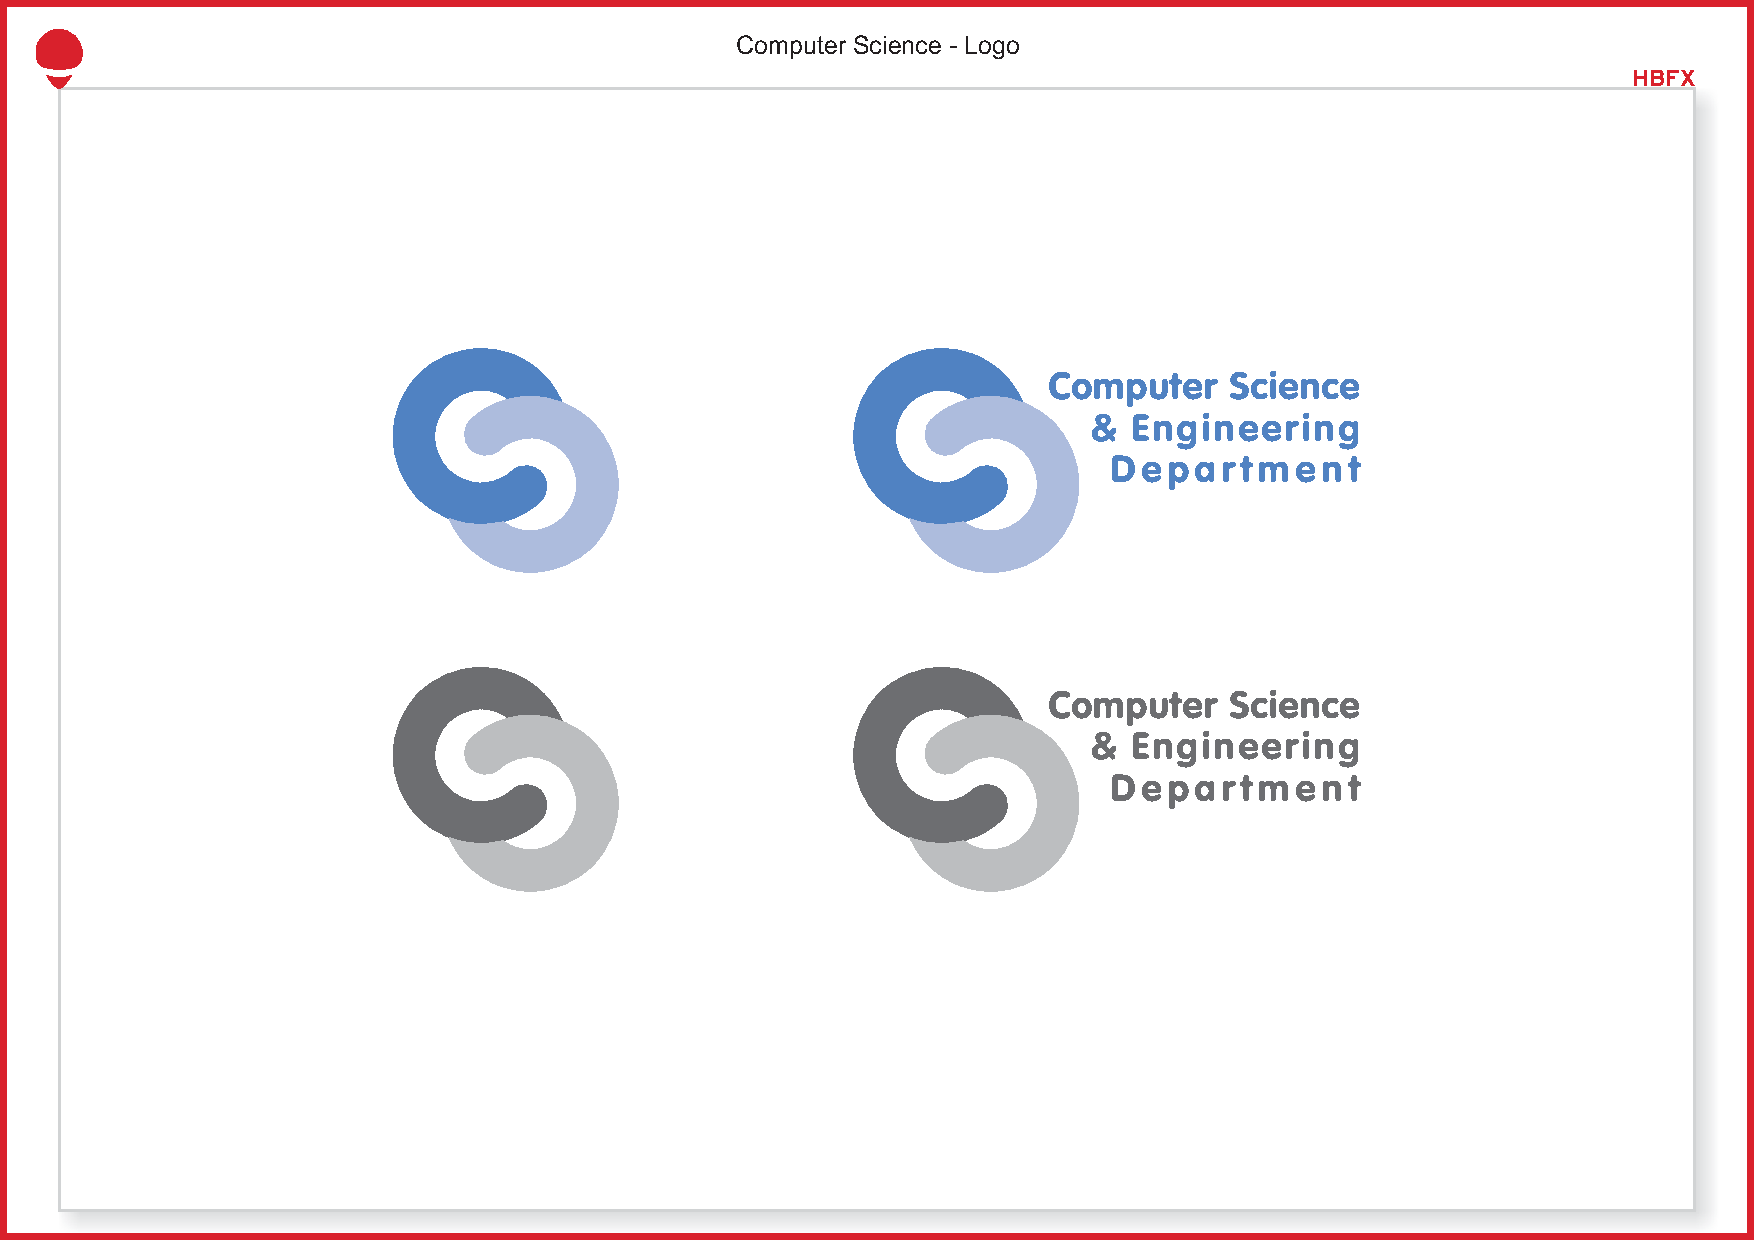
\includegraphics[scale=0.5,trim={14cm 11cm 2cm 5cm},clip=true]{pics/cs-logo.pdf}
\end{tabular}

\vspace{105pt}
{\Huge #2}\\                           % diploma project text
\vspace{40pt}
{\Large #3}\\ \vspace{0pt}  % project title
{\Large #4}\\                          % project subtitle
\vspace{40pt}
{\LARGE \Name}\\                   % student name
\end{center}
\vspace{60pt}
\begin{tabular*}{\textwidth}{@{\extracolsep{\fill}}p{6cm}r}
&{\large\textbf{#5}}\vspace{10pt}\\      % scientific advisor
&{\large \Advisor}                                    % advisor name
\end{tabular*}
\vspace{20pt}
\begin{center}
{\large\textbf{#6}}\\                                % bucharest
\vspace{0pt}
{\normalsize \Year}
\end{center}
\end{titlepage}
}

\newcommand{\frontPageRO}{\frontPage{\UniTextRO}{\DiplomaRO}{\ProjectTitleRO}{\ProjectSubtitleRO}{\AdvisorRO}{\BucRO}}
\newcommand{\frontPageEN}{\frontPage{\UniTextEN}{\DiplomaEN}{\ProjectTitleEN}{\ProjectSubtitleEN}{\AdvisorEN}{\BucEN}}

\linespread{1.15}
\setlength\parindent{0pt}
\setlength\parskip{.28cm}

%% Abstract macro
\newcommand{\AbstractPage}{
\begin{titlepage}
\textbf{\large SINOPSIS}\par
\AbstractRO\par\vfill
\textbf{\large ABSTRACT}\par
\AbstractEN \vfill
\end{titlepage}
}

%% Thank you macro
\newcommand{\ThanksPage}{
\begin{titlepage}
{\noindent \large\textbf{MULȚUMIRI}}\\
\Thanks
\end{titlepage}
}



%%%%%%%%%%%%%%%%%%%%%%%%%%%%%%%%%%%%%%%%%%%%%%%%%%   
%%
%%          End of template definitions
%%   
%%%%%%%%%%%%%%%%%%%%%%%%%%%%%%%%%%%%%%%%%%%%%%%%%%


%%% Puteți elimina aceste linii din lucrare, servesc numai pentru template.
\newcommand{\worktype}[1]{[\textit{#1}] }
\newcommand{\dezvoltare}{\worktype{Dezvoltare de produs}}
\newcommand{\cercetare}{\worktype{Cercetare}}
\newcommand{\ambele}{\worktype{Ambele}}
%%%


%%
%%   Campurile de mai jos trebuie modificate de autor. Modificati doar continutul, nu si numele fiecarei definitii
%%
\newcommand{\ProjectTitleRO}{Implementarea algoritmului Ray Tracing}
\newcommand{\ProjectSubtitleRO}{folosind arhitectura DirectX Raytracing}
\newcommand{\ProjectTitleEN}{Implementation of the Ray Tracing algorithm}
\newcommand{\ProjectSubtitleEN}{using the DirectX Raytracing architecture}
\newcommand{\Name}{Alex-Andrei Cioc}
\newcommand{\Advisor}{Conf. Dr. Ing. Victor Asavei}
\newcommand{\Year}{2024}

% Setări document
\title{Proiect de diplomă}
\author{\Name}
\date{\Year}

%%
%%   Campurile aferente rezumatului
%%
\newcommand{\AbstractRO}{
Algoritmul Ray Tracing este o tehnică de randare a imaginilor care simulează
propagarea și comportamentul razelor de lumină într-o scenă tridimensională. Acesta
este adesea folosit în industria cinematografică pentru a obține imagini fotorealiste.
Până de curând, natura computațională intensivă a acestui algoritm a limitat utilizarea
sa în aplicații interactive, precum jocurile video. Totuși, cu avansul tehnologiei,
utilizarea acestuia a devenit tot mai accesibilă și pentru
aceste aplicații. Suport hardware pentru Ray Tracing în contextul consumatorilor a fost
introdus de NVIDIA în 2018, prin intermediul arhitecturii Turing\footnote{\label{turing}\url{https://images.nvidia.com/aem-dam/en-zz/Solutions/design-visualization/technologies/turing-architecture/NVIDIA-Turing-Architecture-Whitepaper.pdf}. Accesat 10.06.2024.}.
Tot în același an, Microsoft a anunțat DirectX Raytracing\footnote{\label{dxr}\url{https://devblogs.microsoft.com/directx/announcing-microsoft-directx-raytracing/}. Accesat 10.06.2024.} (DXR),
o extensie a API-ului DirectX 12 care permite programatorilor să folosească
Ray Tracing în aplicațiile lor, utilizând hardware-ul compatibil.

Lucrarea de față își propune să studieze și să implementeze
algoritmul Ray Tracing pe un sistem de calcul modern, folosind accelerarea hardware
oferită de arhitectura DirectX Raytracing. Acest algoritm va fi folosit pentru
randarea iluminării unor scene arbitrare, în timp real, oferind o reprezentare fotorealistică a acestora.
În cadrul lucrării se va realiza o analiză a performanțelor implementării curente,
atât a fidelității imaginilor generate, cât și a eficienței spațio-temporale a implementării.
Se vor explora și posibilitățile de optimizare a algoritmului, precum și
modul în care acestea pot fi folosite pentru a îmbunătăți performanțele sistemului.
}

\newcommand{\AbstractEN}{The Ray Tracing algorithm is an image rendering technique that simulates
the propagation and behavior of light rays in a three-dimensional scene. It is
often used in the film industry to achieve photorealistic images.
Until recently, the computationally intensive nature of this algorithm has limited its use
in interactive applications, such as video games. However, with technological advances,
its use has become increasingly accessible for
these applications as well. Hardware support for Ray Tracing in the consumer context was
introduced by NVIDIA in 2018, through the Turing\footref{turing} architecture.
In the same year, Microsoft announced DirectX Raytracing\footref{dxr} (DXR),
an extension of the DirectX 12 API that allows programmers to use
Ray Tracing in their applications, using compatible hardware.

This paper aims to study and implement
the Ray Tracing algorithm on a modern computing system, using the hardware acceleration
provided by the DirectX Raytracing architecture. This algorithm will be used for
rendering the lighting of arbitrary scenes, in real-time, providing a photorealistic representation of them.
The paper will perform an analysis of the current implementation's performance,
both in terms of the fidelity of the generated images and the spatio-temporal efficiency of the implementation.
It will also explore the possibilities for optimizing the algorithm, as well as
how these can be used to improve the system's performance.}

%%
%%   Campurile aferente paginii de multumiri
%%
\newcommand{\Thanks}{Adresez mulțumiri coordonatorului meu de proiect, Conf. Dr. Ing. Victor Asavei, pentru îndrumarea
și sprijinul acordat pe parcursul realizării acestei lucrări, dar și pentru
inspirația și motivația oferită în cadrul cursurilor de Elemente de Grafică pe Calculator.
De asemenea, mulțumesc familiei și prietenilor pentru susținere și încurajare.}

\numberwithin{equation}{section} % for equation numbering

\begin{document}

\frontPageRO
\frontPageEN

\begingroup
\linespread{1}
\tableofcontents
\endgroup

\AbstractPage

% poate fi comentata sau stearsa
\ThanksPage


% Textul licentei incepe de aici 



\chapter{Introducere}\pagestyle{fancy}
% * <marios.choudary@gmail.com> 2018-02-28T11:38:18.106Z:
% 
% > INTRODUCERE
% Am scos de aici referintele la font pentru a nu mai fi dependenti de Calibri. Personal, nici nu sunt sigur ca ajuta prea mult aceasta recomandare si mi se pare bun font-ul default din Latex (Computer Modern). Daca sunteti de-acord, va rog sa stergeti liniile comentate de mai jos, precum si cele referitoare la fontul Calibri din restul documentului.
% 
% ^.


\section{Context}
Industria jocurilor video este una dintre cele mai mari și mai profitabile industrii
de divertisment din lume. În 2021, piața jocurilor video era evaluată la aproximativ
202.64 miliarde de dolari și este estimat să se extindă la o rată anuală compusă de creștere de 10.2\%
în perioada 2022-2030\footnote{\url{https://www.grandviewresearch.com/industry-analysis/gaming-industry}. Accesat 10.06.2024.}.
Această industrie este alimentată de cererea pentru experiențe interactive și captivante,
care să ofere o experiență de joc cât mai realistă și cât mai imersivă. Toate studio-urile
de dezvoltare de jocuri video AAA (i.e., jocuri cu bugete mari și echipe de dezvoltare
extinse) investesc resurse semnificative în dezvoltarea de tehnologii care să le permită
să creeze jocuri cu grafică de înaltă calitate. Aceste tehnologii includ motoare grafice
puternice, care să permită randarea unor scene complexe, cu iluminare realistă și efecte
speciale impresionante. Multe studio-uri folosesc propriile motoare dezvoltate
in-house (e.g., Frostbite de la EA, CryEngine de la Crytek, Anvil de la Ubisoft), dar
există și motoare comerciale, precum Unreal Engine și Unity. Aceste motoare oferă
un set de instrumente și funcționalități care permit dezvoltatorilor să creeze jocuri
video de înaltă calitate, fără a fi nevoie să dezvolte de la zero toate componentele
necesare. O componentă critică a acestor motoare este motorul grafic, care se ocupă
de randarea scenei jocului, de la geometria obiectelor până la iluminare și efecte
speciale. Astfel, programatorii, artiștii, animatorii și designerii de jocuri pot
să se concentreze pe crearea conținutului jocului, fără a fi nevoie să se ocupe
de detalii tehnice ale randării grafice.

\section{Problema}
Tehnica tradițională și cea mai răspândită de randare a imaginilor în jocurile video
este rasterizarea. Această tehnică se bazează pe proiecția obiectelor 3D pe un plan
bidimensional, folosind o serie de algoritmi și tehnici pentru a simula iluminarea și
efectele speciale. Rasterizarea este o tehnică eficientă și rapidă, care permite
randarea unui număr mare de obiecte în timp real, dar are și limitări. Una dintre
cele mai mari limitări ale rasterizării este incapacitatea de a simula iluminarea
globală, care este esențială pentru obținerea unor imagini fotorealiste. De asemenea,
reflexiile și refracțiile pot fi doar aproximate, de exemplu prin tehnici de cubemapping
sau screen-space reflections. Aceste tehnici sunt eficiente, dar nu oferă rezultate
realistice, iar în multe cazuri pot fi observate artefacte vizuale care afectează
calitatea imaginii.

În continuare se evidențiază aceste limitări (care nu sunt deloc exhaustive) ale
rasterizării, prin comparație cu tehnica de Ray Tracing (așa numita \textit{RTX} în
jocurile sponsorizate de Nvidia).
Comparând Figurile~\ref{fig:ssr-good} și~\ref{fig:ssr-bad}, se observă neajunsul
reflexiilor în screen space. Atâta timp cât obiectele reflectate se află în viewport,
reflexiile sunt corecte și realiste. Însă, dacă obiectele ies din viewport, reflexiile
se pierd, ceea ce duce la o imagine nerealistă. Un alt exemplu și mai elocvent este
ilustrat în Figura~\ref{fig:bf5-rtx}, unde imaginea randată cu Ray Tracing redă
reflexii ale exploziei care nu este vizibilă decât parțial în cadru.

\begin{figure}[ht]
	\centering
	\includegraphics[width=0.8\textwidth]{pics/mc-ssr-good.png}
	\caption{Screen space reflections în Minecraft\protect\footnotemark}
	\label{fig:ssr-good}
\end{figure}
\footnotetext{\label{continuum}Shader folosit: \textcopyright \url{https://continuum.graphics/}. Accesat  10.06.2024.}

\begin{figure}[ht]
	\centering
	\includegraphics[width=0.8\textwidth]{pics/mc-ssr-bad.png}
	\caption{Artefacte vizuale în screen space reflections\protect\footref{continuum}. Se poate observa cum
		reflexiile se pierd dacă obiectele reflectate ies din viewport}
	\label{fig:ssr-bad}
\end{figure}

\begin{figure}[ht]
	\centering
	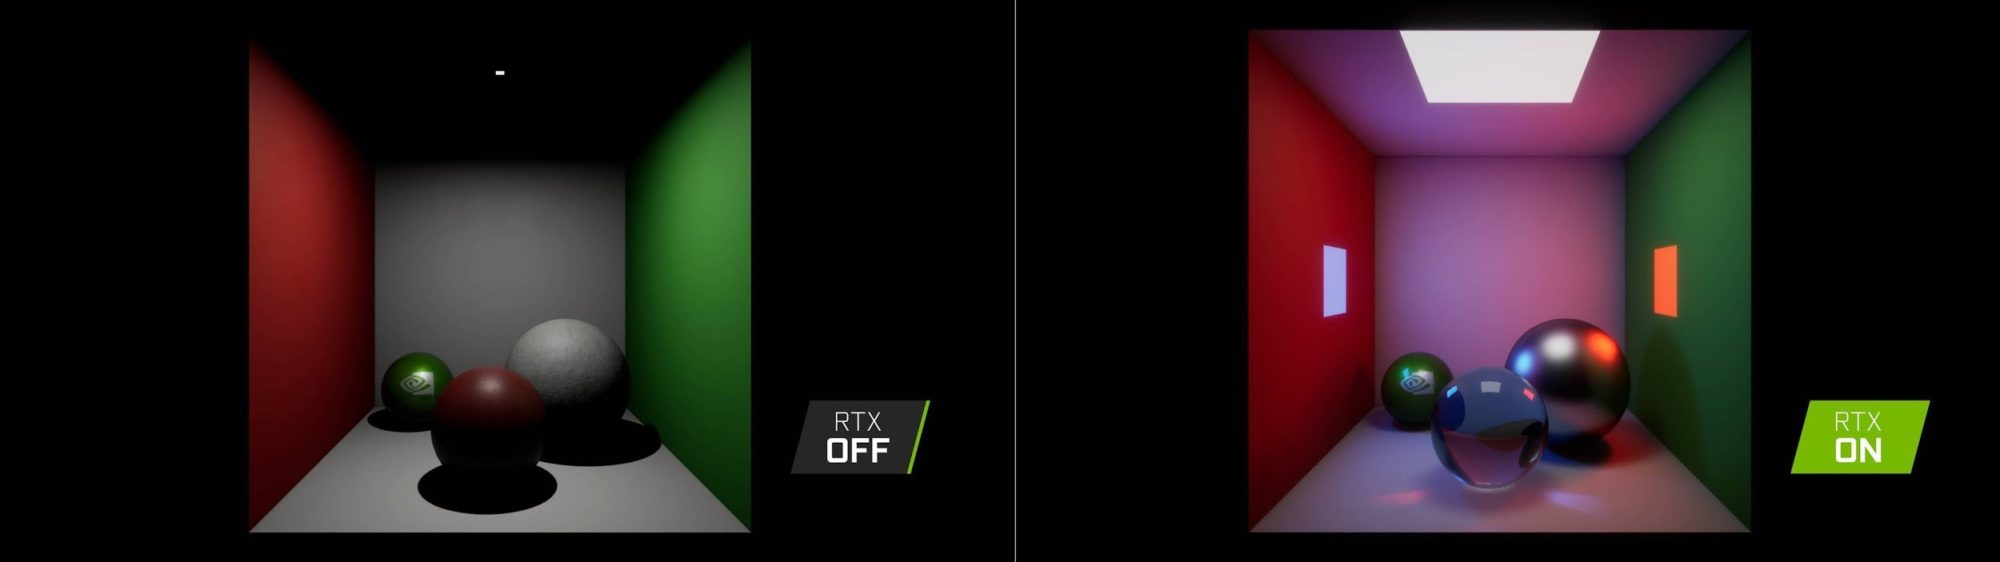
\includegraphics[width=0.8\textwidth]{pics/cornell-raster.jpg}
	\caption{Iluminarea globală este absentă în imaginea randată cu rasterizare\protect\footnotemark}
	\vspace{1cm}
	\label{fig:cornell-raster}
\end{figure}
\footnotetext{\textcopyright Nvidia Corporation: \url{https://blogs.nvidia.com/blog/geforce-rtx-real-time-ray-tracing/}. Accesat 10.06.2024.}

\begin{figure}[ht]
	\centering
	\begin{subfigure}[h]{0.45\linewidth}
		\centering
		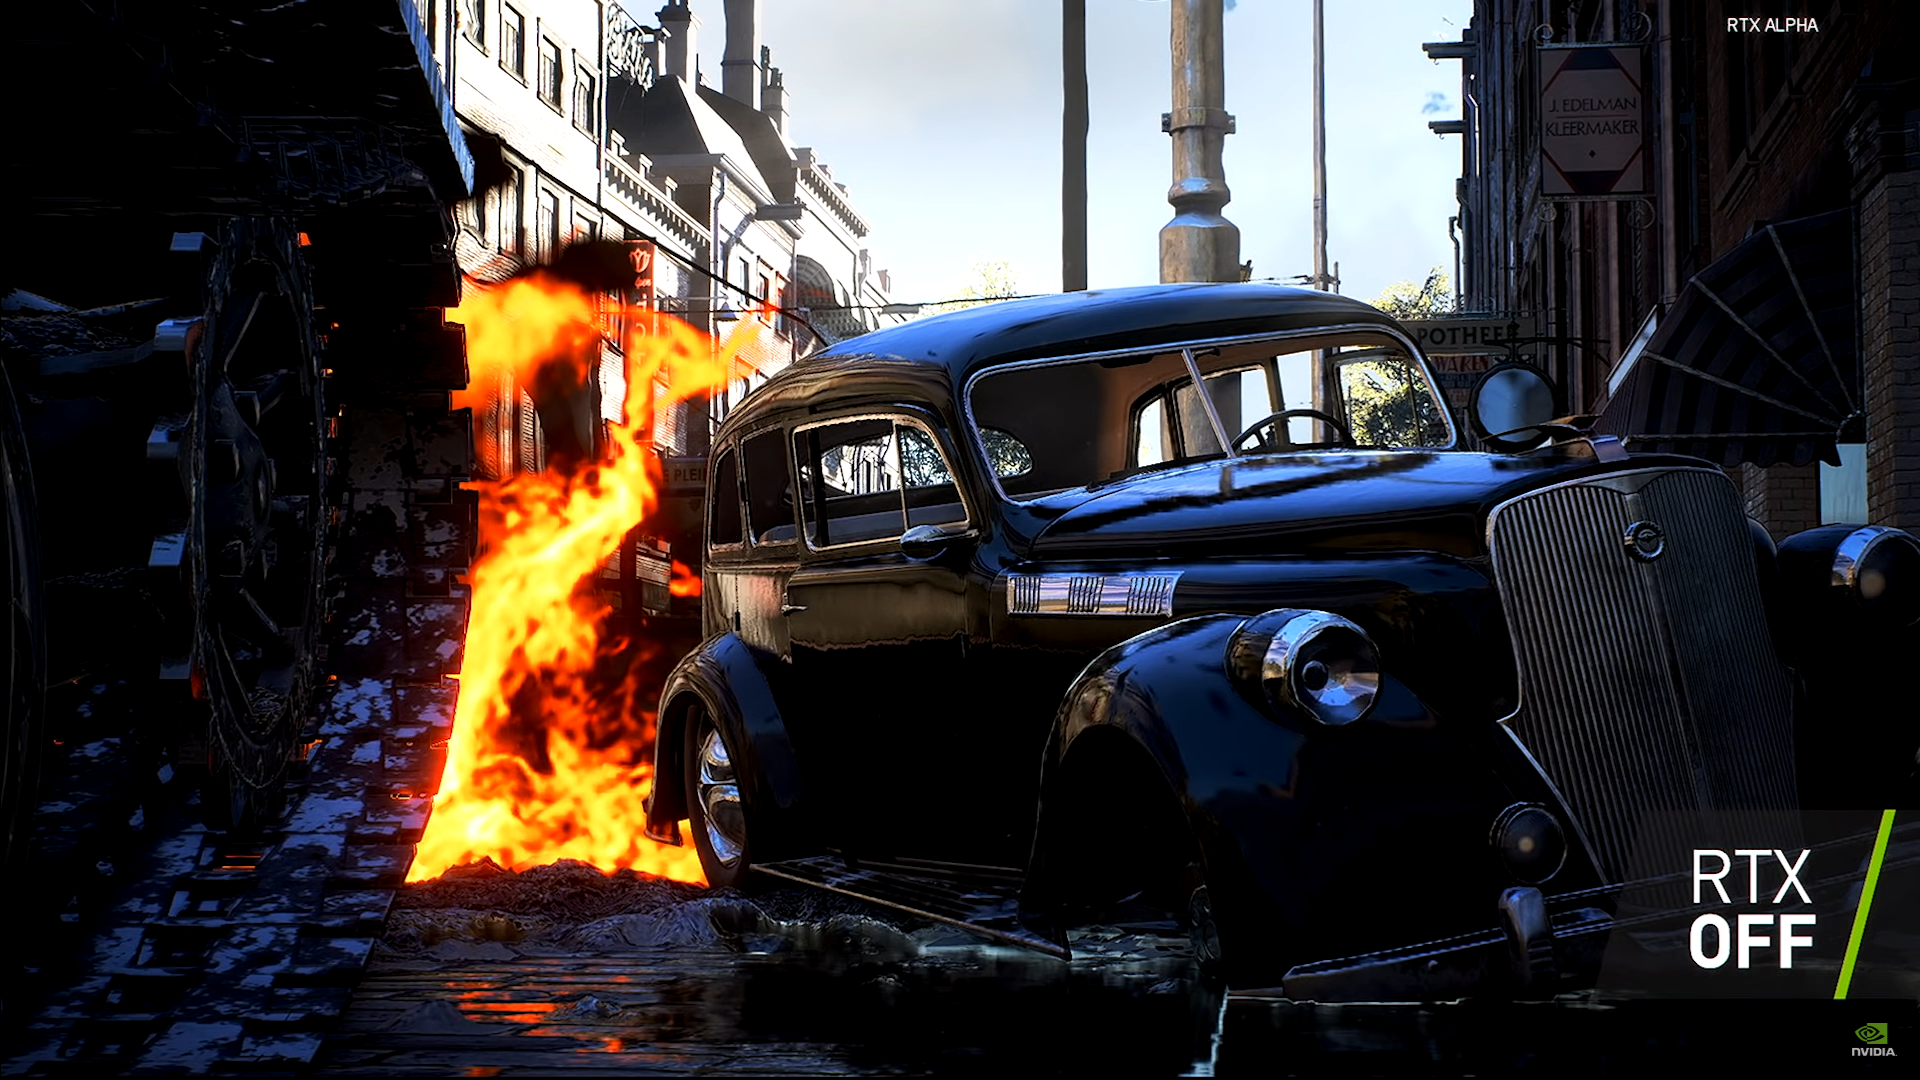
\includegraphics[width=\linewidth]{pics/bf5-rtx-off.png}
		\caption{RTX off}
	\end{subfigure}
	\hfill
	\begin{subfigure}[h]{0.45\linewidth}
		\centering
		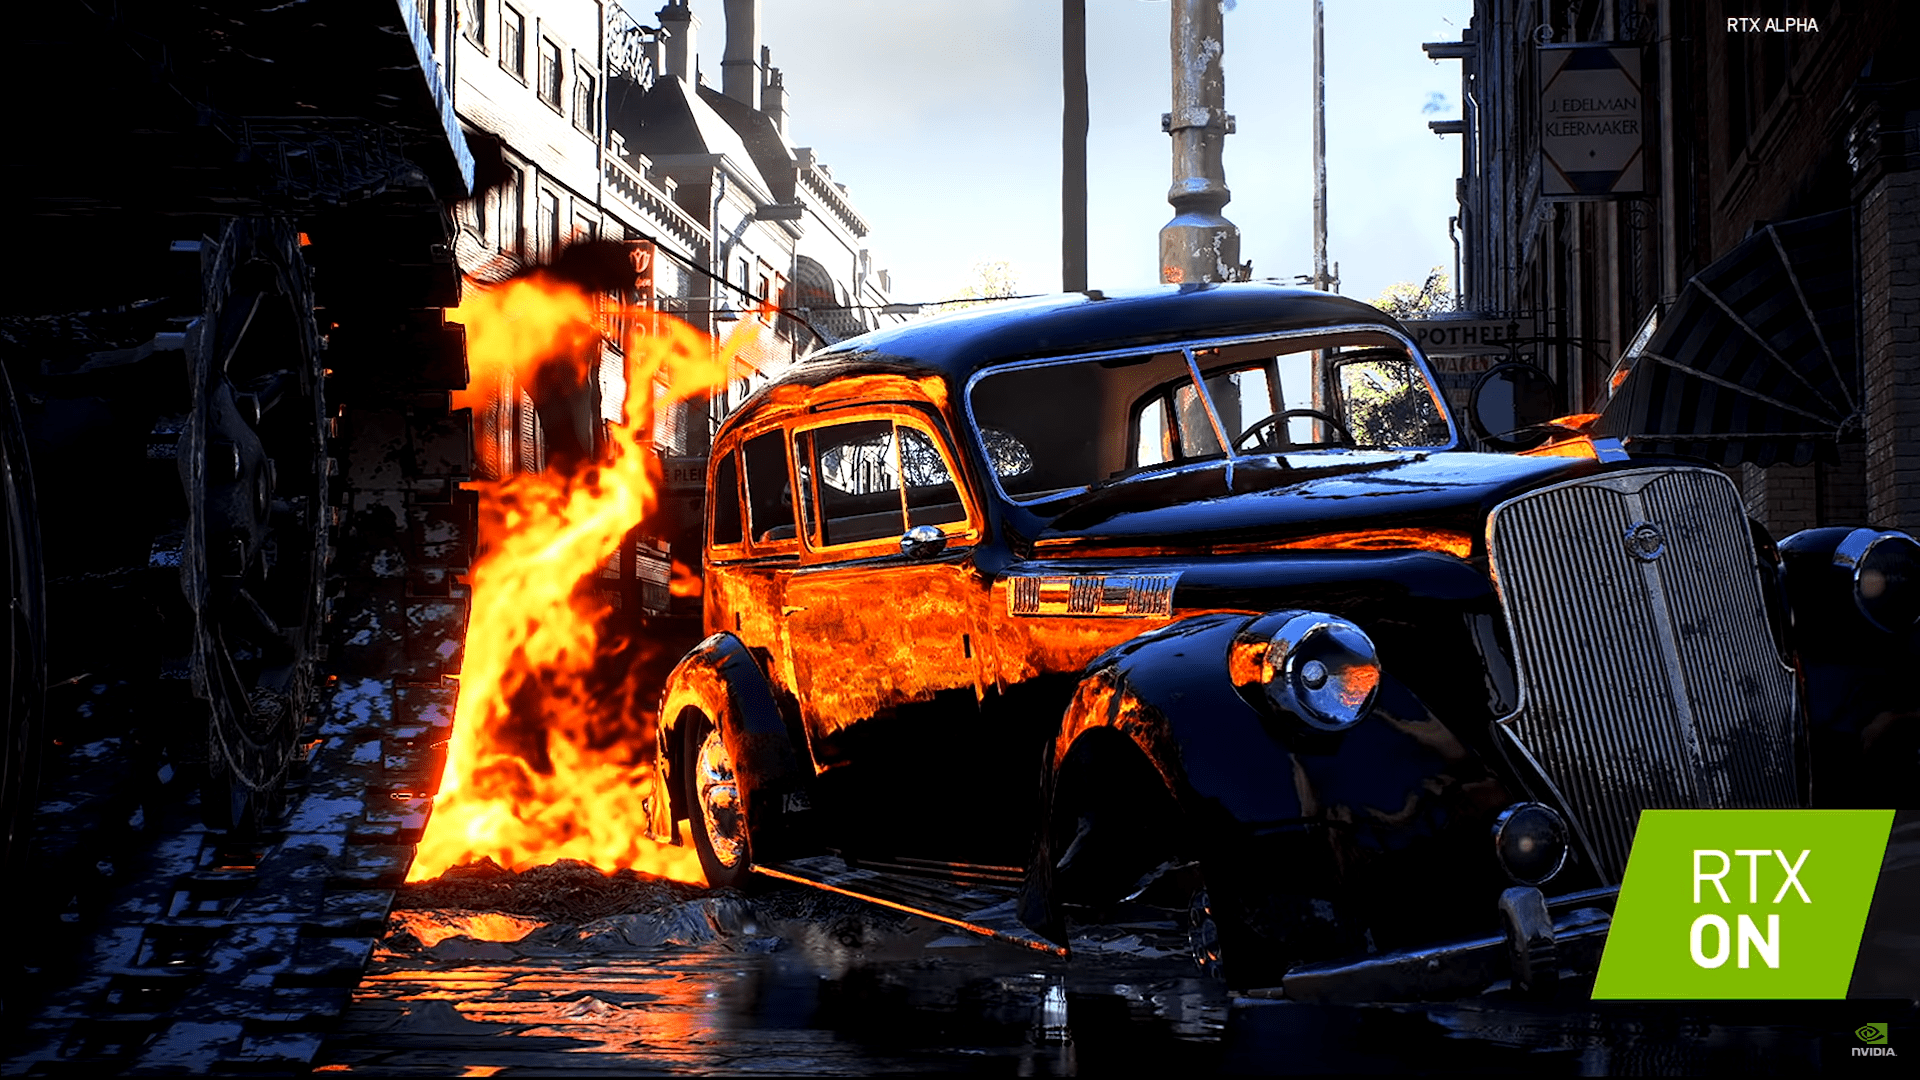
\includegraphics[width=\linewidth]{pics/bf5-rtx-on.png}
		\caption{RTX on}
	\end{subfigure}
	\caption{Comparație RTX on/off în Battlefield V\protect\footnotemark}
	\label{fig:bf5-rtx}
\end{figure}
\footnotetext{\textcopyright Nvidia Corporation: \url{https://www.youtube.com/watch?v=WoQr0k2IA9A}. Accesat 10.06.2024.}

Am văzut cum tehnica de Ray Tracing poate oferi rezultate mult mai realiste
decât rasterizarea, dar această tehnologie vine cu un cost.
Algoritmul Ray Tracing este computațional intensiv, deoarece necesită
calcularea intersecțiilor mai multor raze de lumină pentru fiecare pixel cu obiectele din scenă
și calcularea contribuției acestora la culoarea pixelului. Pentru a obține o imagine
de calitate, este nevoie de un număr mare de raze de lumină și tehnici de denoising,
ceea ce face ca algoritmul să fie greu de balansat între fidelitate și performanță.

\section{Obiective}

Scopul acestei lucrări este de a cerceta și implementa algoritmul Ray Tracing în
context de timp real și a evalua performanțele acestuia, prin comparație cu
implementări destinate producției cinematografice. Eforturile vor fi concentrate
pe implementarea unui motor grafic simplu, cu câteva funcționalități de bază:
\begin{itemize}
	\item Controale de cameră simple (mișcare, rotire)
	\item Randarea obiectelor definite ca mesh-uri triunghiulare
	\item Randarea obiectelor definite prin funcții implicite (e.g., sfere, planuri)
	\item Suport pentru materiale PBR (Physically Based Rendering)
	\item Meniu de configurare a mai multor parametri (e.g., pentru scenă,
	      configurarea algoritmului etc.),
\end{itemize}
precum și a unor efecte de iluminare care să ofere o imagine fotorealistică a scenei:
\begin{itemize}
	\item Iluminare globală
	\item Reflexii și refracții
	\item Umbre.
\end{itemize}
De asemenea, vom explora și implementa tehnici de optimizare a algoritmului propriu-zis,
pe care le vom evalua în contextul de performanță și fidelitate obținute.

În final, dorim să obținem o implementare eficientă, care să țintească un frametime de 33.3ms
(30 de cadre pe secundă) la o rezoluție Full HD (1920x1080), pentru hardware entry-level cu suport pentru
DirectX Raytracing (e.g., Nvidia GeForce RTX 2060).

\subsubsection*{}

\section{Soluția propusă}
Soluția propusă este un motor grafic simplu de utilizat. Din perspectiva utilizatorului,
acesta are un meniu din care poate configura diverși parametri ai algoritmului
de Ray Tracing, precum și ai scenei. Utilizatorul poate încărca scene predefinite
și poate interacționa cu acestea folosind controalele de cameră.

La nivel de bază, motorul grafic conține două implementări din clasa algoritmilor
de Ray Tracing. Prima este o versiune simplă a algoritmului original descris de
Whitted (1979)~\cite{Whitted}, peste care se aplică modelul clasic de iluminare
Phong (1975)~\cite{Phong}. Această implementare a fost adaptată din codul sursă
suport oferit de Microsoft~\cite{Schelet}.
A doua implementare este scrisă de la zero și folosește algoritmul de tip Monte Carlo
Path Tracing pentru a rezolva ecuația de iluminare globală propusă de Kajiya (1986)~\cite{Kajiya}.
Fără a intra în prea multe detalii tehnice (vezi capitolul \ref{sec:stateoftheart}),
această ecuație descrie cantitatea de lumină emisă dintr-un punct de pe o suprafață,
de-a lungul unei direcții de vizualizare, dându-se o funcție de distribuție a luminii
și un BRDF (Bidirectional Reflectance Distribution Function) pentru materialul de pe
suprafață. Ecuația conține o integrală de suprafață (peste emisfera unitate), care
integrează contribuțiile din toate direcțiile. Pentru eficiență, această integrală
este eșantionată folosind tehnici de eșantionare bazate pe importanță, descrise în capitolul \ref{sec:stateoftheart}.
Totuși, numărul de eșantioane per pixel rămâne în continuare foarte limitat, din
cauza bugetului de calcul (nu depășește 16 eșantioane per pixel). Pentru a reduce
în continuare varianța (manifestată prin zgomot în imaginea finală), se folosește
un algoritm de denoising în faza de post procesare. Mai multe detalii tehnice
despre implementare sunt prezentate în capitolul \ref{sec:implementare}.

Algoritmul de Path Tracing folosește un sistem de materiale diferit de cel folosit
de algoritmul Whitted. Dacă acesta din urmă este limitat de modelul simplu de iluminare
Phong, Path Tracing folosește un model PBR (Physically Based Rendering) inspirat de
cel introdus de Burley în 2012~\cite{Disney}, pentru a fi folosit în producția filmelor
marca Walt Disney Animation Studios. Varianta implementată în această lucrare este
augmentată cu o componentă de transmisie, descrisă într-un curs organizat de Hill et al. la conferința SIGGRAPH din 2015~\cite{DisneyBSDF}.
Acest model este mult mai complex,
având la bază un BSDF (Bidirectional Scattering Distribution Function - oferă și
o componentă de transmisie a luminii prin materiale) care descrie cum un material
interacționează cu lumina incidentă. Fiind totuși folosit în producția cinematografică,
modelul se concentrează pe a avea o interfață cât mai intuitivă pentru artistul
grafic, deviând puțin de la un model fizic strict. Bazele teoretice și implementarea acestui model
PBR sunt descrise în secțiunile \ref{sec:stateoftheart} și \ref{sec:implementare}.

Pentru evaluare se va
face o comparație între cei doi algoritmi de Ray Tracing. Se va mai observa și
capabilitatea algoritmului de Path Tracing de a simula surse de lumină de tip
area light, care sunt dificil de modelat în algoritmul Whitted.
Scena de test prezintă materialele PBR, exclusive pentru algoritmul de Path Tracing.
Aceasta conține mai multe obiecte definite prin suprafețe implicite și obiecte
definite ca mesh-uri triunghiulare. Se va evalua performanța de rulare și
stabilitatea imaginii generate pentru diferite setări ale algoritmului de Path Tracing.

\section{Rezultatele obținute}

Rezultatele obținute sunt încurajatoare, deși mai este loc de multe îmbunătățiri.
În primul rând, aplicația este ușor de folosit, este stabilă și destul de configurabilă.
Algoritmul implementat are o fidelitate bună, iar sistemul de materiale este de calitate.

Din păcate, obiectivul de performanță nu este atins decât pentru un număr foarte
mic de eșantioane per pixel (1-4). Situația se imbunătățește semnificativ dacă
se activează varianta progresivă a algoritmului, însă, în absența unui denoiser
cu informație de vectori de mișcare, imaginea finală este o simplă agregare a
mai multor cadre, ceea ce duce la un efect de blur pronunțat pentru obiectele în mișcare.
Implementarea unei astfel de soluții este primul lucru pe lista de îmbunătățiri
viitoare.

Rezultate calitative și interpretarea acestora sunt prezentate în capitolul \ref{sec:evaluare}.

\section{Structura lucrării}

Vreau să încep prin a clarifica faptul că această lucrare nu își propune să introducă
noi metode sau concepte în domeniul graficii pe calculator. Scopul acesteia
este de a experimenta și de a înțelege mai bine tehnologiile existente, precum
și de a pune în practică teoria care stă la baza acestora. Lucrarea este structurată
într-o parte teoretică inițială, menită să familiarizeze cititorul printr-o introducere lină
în conceptele care stau la baza algoritmului de Path Tracing, și o parte practică,
care se concentrează pe utilizarea API-ului DirectX12 pentru a implementa algoritmul
cu accelerare hardware. Conceptele tehnice din urmă nu vor fi prezentate
într-o lumină precisă, ci mai degrabă într-un mod simplificat și intuitiv, din
perspectiva unui tool care folosit pentru implementarea algoritmului în sine.

În capitolul~\ref{sec:motivatie} este descris contextul actual în care se plasează
eforturile din domeniu, din perspectiva industriilor de gaming și de cinematografie,
și se prezintă motivațiile principale pentru a continua avansurile în cercetare.

În capitolul~\ref{sec:stateoftheart} se analizează stadiul curent al cercetărilor
în domeniul algoritmilor de Path Tracing, cu focus pe optimizări pentru timp real.
Aici se prezintă teoria care stă la baza lucrării și se explică în detaliu fiecare
aspect.
De asemenea, se poziționează lucrarea de față în acest peisaj și se conturează
aspectul didactic al acesteia.

În capitolul~\ref{sec:solutie} se prezintă funcționalitățile prezente în aplicație,
precum și punerea teoriei în practică. Tot aici se prezintă sistemul de materiale
specific folosit și ecuațiile care îl definesc. De asemenea, se descrie arhitectura
generală a motorului grafic, cu accent pe componentele modificate și adăugate
față de schelet~\cite{Schelet}.

Capitolul~\ref{sec:implementare} detaliază utilizarea API-urilor DirectX 12 și DXR
pentru implementarea algoritmilor de Ray Tracing cu accelerare hardware. Accentul
este pus pe transpunerea aspectelor teoretice în cod și pe deciziile de design luate pentru a obține o implementare
eficientă și ușor de înțeles. Tot aici se notează și dificultățile întâmpinate
și compromisurile făcute pentru a obține un echilibru între fidelitate și performanță.

Capitolul de evaluare \ref{sec:evaluare} prezintă rezultatele obținute
în urma testelor efectuate. Se analizează
performanțele sistemului, fidelitatea imaginilor generate și se fac comparații
între cei doi algoritmi de Ray Tracing. De asemenea, se analizează impactul pe
care îl au diferitele optimizări asupra stabilității imaginilor generate.

Ultimul capitol ~\ref{sec:concluzii} conține concluziile trase din
rezultatele obținute și se analizează calitativ produsul final. De asemenea, se
discută posibile direcții de dezvoltare pe termen scurt și termen lung și se oferă o perspectivă asupra
importanței acestei lucrări în contextul cercetării în domeniul graficii pe calculator.

Extrase de cod și imagini detaliate sunt oferite în \hyperref[anexa]{anexă}.

\chapter{\label{sec:motivatie}Motivație de cercetare}

Proiectul de față cercetează tehnici de randare a imaginilor în timp real. Acest
domeniu este de mare interes pentru industria jocurilor video, care investesc
resurse semnificative în dezvoltarea de motoare grafice puternice.

Un studiu de caz
recent\footnote{\label{vnextglobal}\url{https://vnextglobal.com/category/blog/game-development-cost-an-in-depth-analysis}. Accesat 19.06.2024.}
analizează costurile de dezvoltare ale unui joc video AAA. Două dintre jocurile
cu cel mai mare buget sunt Grand Theft Auto V și Cyberpunk 2077, care investit
peste 270, respectiv 300 milioane de dolari în dezvoltare și marketing. O parte
importantă a acestor bugete a fost alocată pentru dezvoltarea motoarelor grafice
proprietare.

RAGE (Rockstar Advanced Game Engine) este motorul grafic folosit
de Rockstar Games pentru jocurile sale de tip open-world, precum GTA V. Acesta a
trebuit să fie adaptat pentru portarea jocului pe consolele de nouă generație
(PS4 și Xbox One) și pentru PC, suportând rezoluții de până la 4K pe PC.\footnote{\url{https://www.eurogamer.net/digitalfoundry-2015-grand-theft-auto-5-pc-face-off}. Accesat 19.06.2024.}
RAGE a primit o iterație semnificativă odată cu lansarea Red Dead Redemption 2 în 2018
(un alt joc cu un buget de dezvoltare mare, de peste 100 milioane de dolari\footref{vnextglobal}),
care a adus noi tehnici de randare precum suport PBR, nori volumetrici și iluminare globală
precalculată\footnote{\url{https://www.eurogamer.net/digitalfoundry-2017-red-dead-redemption-2-trailer-tech-analysis}. Accesat 19.06.2024.}\footnote{\url{https://www.eurogamer.net/digitalfoundry-2018-red-dead-redemption-2-tech-analysis}. Accesat 19.06.2024.}.

Cyberpunk 2077 a început dezvoltarea folosind un nou motor REDengine 3\footnote{\url{https://www.engadget.com/2013-02-01-cd-projekt-red-introduces-redengine-3-latest-iteration-of-in-ho.html}. Accesat 19.06.2024.},
creat special pentru a îmbina o lume de joc vastă și detaliată cu o poveste complexă,
bazată pe deciziile jucătorului. Totuși, acest motor nu era destul de flexibil pentru
a suporta toate cerințele jocului\footnote{\url{https://www.superjumpmagazine.com/why-cd-projekt-reds-switch-to-unreal-engine-is-a-big-deal/}. Accesat 19.06.2024.}
(precum first person shooting și condus de mașini),
așa că au început lucrul la o nouă versiune, REDengine 4, folosind un grant de 7 milioane
de dolari de la guvernul polonez\footnote{\label{UE5}\url{https://www.wipo.int/edocs/mdocs/mdocs/en/wipo_smes_ge_20/wipo_smes_ge_20_p3.pdf}. Accesat 19.06.2024.}.
Nici acest proces nu a fost fără dificultăți (lansarea jocului a fost dezastruoasă
și plină de bug-uri\footnote{\url{https://gamerant.com/cyberpunk-2077-review-bombing-negative-impact-bad-example/}. Accesat 19.06.2024.},
iar studio-ul a decis după lansare să tranziționeze către Unreal Engine 5\footref{UE5} pentru jocurile viitoare),
dar a permis jocului să fie primul care să ofere iluminare realizată integral cu Path Tracing\footnote{\url{https://www.tomshardware.com/news/cyberpunk-277-rt-overdrive-available-to-all}. Accesat 19.06.2024.}.
Acest lucru a fost posibil datorită colaborării cu Nvidia\footnote{\url{https://www.nvidia.com/en-us/geforce/news/cyberpunk-2077-nvidia-partnership-ray-tracing/}. Accesat 19.06.2024.},
care a oferit suport în implementarea tehnologiei RTX în REDengine 4.

Am văzut astfel ce eforturi depun companiile mari pentru a aduce fidelitate grafică
în jocurile lor. Un studiu realizat de Tondello și Nacke în 2019\cite{Tondello} pe
două eșantioane de gameri a arătat că majoritatea jucătorilor sunt interesați
de aspectele estetice ale jocurilor video, precum grafica și sunetul. În alt
studiu realizat de Katja et al. în 2022\cite{Katja}, s-a analizat concepția
literaturii asupra realismului în jocuri video. Deși s-a concluzionat că acest
termen nu este bine definit de multe ori, cel mai adesea în literatură acesta
se referă, printre altele, la fidelitatea grafică a jocului.

Așadar, unul dintre cele mai importante aspecte ale unui joc video, în relație cu
experiența jucătorului, este fidelitatea grafică\footnote{\url{https://goombastomp.com/why-good-graphics-matter-in-video-games-enhancing-the-visual-experience/}. Accesat 19.06.2024.}. Aceasta este influențată de
calitatea modelelor 3D, a texturilor, a animațiilor, a efectelor speciale, dar
și de iluminare. Iluminarea este un aspect critic al fidelității grafice, deoarece
aceasta influențează cum percepem obiectele din joc. O lume frumos modelată nu
poate avea un impact vizual puternic dacă nu este pusă într-o "lumină bună".
Această "lumină bună" izvorăște adânc din tehnologiile folosite de motorul grafic
pentru a da valoare obiectelor în scenă. Deși există multe stiluri atractive de
a prezenta o scenă (e.g., cel-shading, pixel art), realismul este unul dintre cele
mai populare, deoarece oferă o experiență de joc mai imersivă. Clasa de algoritmi
de Ray Tracing este una dintre cele mai bune tehnici de a obține realism în jocuri,
însă aceasta vine cu un cost computațional ridicat. De aceea, eforturi de cercetare
în domeniu sunt necesare pentru a găsi soluții care să ofere un compromis între
fidelitate și performanță\footnote{\url{https://blogs.nvidia.com/blog/rtx-real-time-ray-tracing/}. Accesat 19.06.2024.}.
Ca referință, NVIDIA oferă public multe studii de cercetare și articole științifice
publicate de echipa lor de cercetare\footnote{\url{https://research.nvidia.com/labs/rtr/publication/}. Accesat 19.06.2024.}.
Marea majoritate se concentrează pe optimizarea tehnicilor de prezentare grafică
(Path Tracing reprezentând o parte importantă a acestora) și oferă o privire de
ansamblu asupra eforturilor de cercetare în domeniu.

Ca o ultimă observație, să ne imaginăm că fidelitatea cu care se realizează
producția filmelor de animație ar putea fi adusă în jocurile video. Din cealaltă
perspectivă, filmele video ar putea fi randate în timp real, fără consum enorm
de energie. Aceste avantaje ar reduce costurile de producție și ar accelera
procesul de dezvoltare a filmelor. Eforturile de cercetare în domeniu sunt
necesare pentru a face aceste viziuni realitate.

La nivel personal, această lucrare reprezintă o oportunitate de a învăța și
de a experimenta cu tehnologii avansate de randare a imaginilor. Scriu lucrarea
de față în ideea în care dacă ar fi să o iau de la început și să învăț aceste concepte
din nou, aș vrea să am la dispoziție un ghid simplu și intuitiv care să mă
ajute să înțeleg teoria și să o pun în practică. În cercetarea efectuată de mine
nu am găsit o introducere completă și accesibilă, mai ales în contextul API-urilor
de ultimă generație precum DirectX 12. Așadar, această lucrare își propune să
fie un astfel de ghid, care să ofere cititorului o introducere lină și încurajatoare.

\chapter{\label{sec:stateoftheart}Metode Existente}

Literatura de specialitate din domeniul graficii pe calculator este vastă. Există
multe metode de randare a imaginilor și se dă o luptă constantă între a balansa
performanța cu fidelitatea. Direcția de cercetare cea mai proeminentă se axează
în jurul metodelor de tip Monte Carlo, care reprezintă state-of-the-art în
domeniu. Deși conceptele care vor fi prezentate nu sunt noi (metode de rezolvare
a ecuației de randare există de aproape 40 ani), apar întotdeauna noi tehnici
de optimizare și de îmbunătățire a performanțelor de convergență și de stabilitate
a algoritmilor. Pentru o privire mai detaliată asupra avansurilor curente și asupra
viitorului cercetării în domeniu, notițele de curs din 2019 ale lui Keller et al.~\cite{Keller}
sunt o resursă excelentă. De asemenea, pentru o privire de ansamblu și de actualitate asupra tehnologiilor
de accelerare în timp real folosite în industria jocurilor video (mai ales cele de la Nvidia - RTXDI, RTXGI, NRD, DLSS), recomand prezentarea
de la GTC și GDC 2022 a lui Clarberg et al.~\cite{Clarberg2022}, din partea Nvidia Corporation.

În continuare, vom prezenta fundamentele teoretice ale clasei de
algoritmi Ray Tracing și vom analiza cele mai importante metode existente.

\section{Rasterizare}

Pentru a avea un punct de plecare, vom vorbi puțin și despre rasterizare.
Aceasta este metoda de bază folosită în majoritatea jocurilor video din trecut și
de astăzi. Ea este reprezentată ca un stagiu fix (neprogramabil) din pipeline-ul
de randare al GPU-ului (vezi Figura~\ref{fig:pipeline}), care transformă primitivele definite vectorial (triunghiuri,
linii, puncte) în pixeli pe ecran. Acest proces este foarte eficient, deoarece
folosește hardware specializat pentru a face calculele necesare.

Etapele principale ale rasterizatorului sunt\footnote{\url{https://learn.microsoft.com/en-us/windows/uwp/graphics-concepts/rasterizer-stage--rs-}. Accesat 19.06.2024.}:
\begin{enumerate}
	\item \textit{Clipping} - eliminarea primitivelor care nu se află în câmpul vizual (view frustum)
	\item \textit{Perspective division} - împărțirea coordonatelor omogene pentru a obține coordonatele normalizate (NDC)
	\item \textit{Transformarea viewport} - transformarea coordonatelor normalizate în coordonate ecran
	\item \textit{Rasterizarea} - determinarea pixelilor acoperiți de primitivă.
\end{enumerate}
După rasterizare urmează etapa programabilă de pixel shader, unde se calculează de
obicei efecte de iluminare, umbre, texturi etc.
Un exemplu de imagine randată cu rasterizare se poate vedea în Figura~\ref{fig:rasterization}.

\begin{figure}[ht]
	\centering
	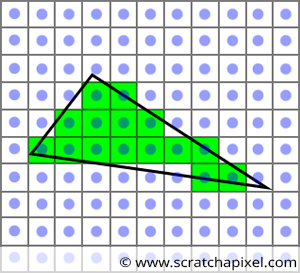
\includegraphics[width=0.5\textwidth]{pics/rasterization.png}
	\caption{Exemplu de imagine randată folosind rasterizare\protect\footnotemark}
	\label{fig:rasterization}
\end{figure}
\footnotetext{\copyright\url{https://www.scratchapixel.com/}. Accesat 19.06.2024.}

Deși rasterizarea este foarte eficientă, ea are multe limitări. Efectele de iluminare
pot fi doar aproximate, iar umbrele și reflexiile/refracțiile sunt greu de realizat. Motoarele
grafice folosesc metode de baking\footnote{\url{https://www.flipcode.com/archives/Light_Mapping_Theory_and_Implementation.shtml}. Accesat 20.06.2024.} pentru a precalcula iluminarea statică în scenă
la o calitate bună (folosind alte metode, e.g., radiosity~(\ref{sec:radiosity})), dar iluminarea dinamică și umbrele dinamice sunt randate la
calitate scăzută. Printre tehnicile folosite pentru a îmbunătăți aspectul vizual
al jocurilor se numără ocluzia ambientală, shadow mapping, screen-space reflections,
cubemap reflections, light probes, lightmaps, etc.

\section{Ray Tracing}

În sens general, Ray Tracing reprezintă o clasă de algoritmi și tehnici de randare
a imaginilor care au la bază simularea transportului luminii într-o scenă.
Spre deosebire de rasterizare, care proiectează obiectele 3D pe un plan 2D, Ray
Tracing rezolvă problema vizibilității trasând raze din ochiul camerei în scenă
și calculând intersecțiile cu geometria 3D. Vom prezenta în continuare diferite
variațiuni ale acestui algoritm.

\subsection*{Ray Casting}

Prima aplicație a algoritmului în
grafica pe calculator a fost făcută de Appel în 1968~\cite{Appel} - în acest
context algoritmul era nerecursiv. Razele primare calculau intersecțiile cu obiectele
din scenă, iar razele secundare erau folosite pentru a calcula umbre. Această
variantă nerecursivă a algoritmului este cunoscută sub numele de Ray Casting.
Figura~\ref{fig:raycasting} prezintă vizualizarea algoritmului.

Datorită simplității sale, Ray Casting este un algoritm foarte eficient (fiind ușor
paralelizabil), însă nu oferă în sine niciun efect de iluminare - este un algoritm
de vizibilitate.

\begin{figure}[ht]
	\centering
	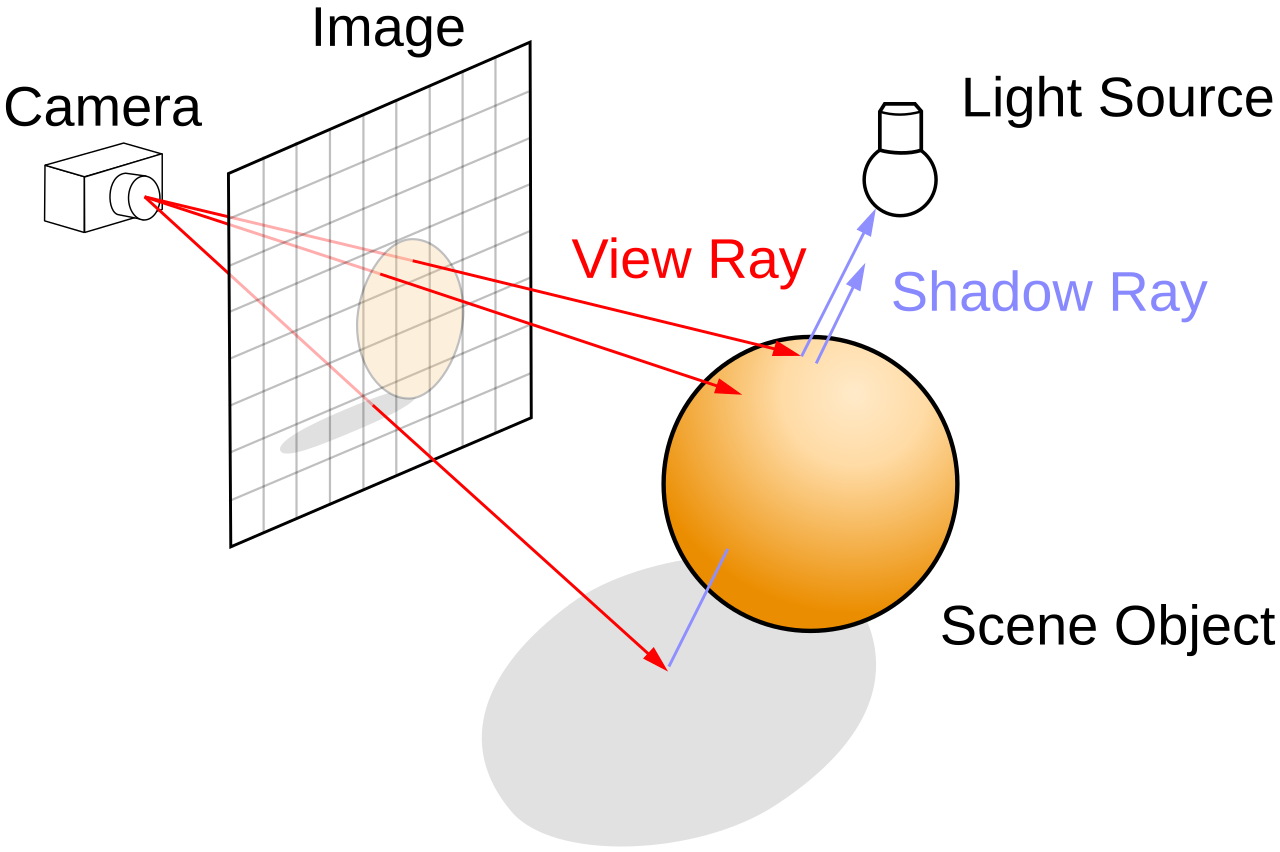
\includegraphics[width=0.5\textwidth]{pics/appel.png}
	\caption{Algoritmul Ray Casting. Cu roșu sunt reprezentate razele primare, iar cu albastru razele secundare\protect\footnotemark}
	\label{fig:raycasting}
\end{figure}
\footnotetext{\label{fn:wiki}\copyright\url{https://en.wikipedia.org/}. Accesat 20.06.2024.}

\subsection*{Ray Tracing Recursiv}

Algoritmul inițial de Ray Casting nu putea calcula efecte precum reflexii și refracții.
Pentru acestea, era nevoie de o variantă recursivă a algoritmului, care să calculeze
traiectoria razei de-a lungul mai multor puncte din scenă și să țină cont de
contribuțiile tuturor suprafețelor intersectate. Această variantă a fost prezentată
în practică pentru prima dată de Whitted (1979)~\cite{Whitted}. Astfel, fiecare
intersecție, se pot genera 3 noi raze: o rază de reflexie, o rază de refracție și
o rază de umbrit. Adâncimea recursivității este, evident, limitată, căci complexitatea
crește exponențial. Este de remarcat faptul că efectele de reflexie, refracție, umbrire,
precum și alte efecte specifice (e.g., blur, depth of field) pot fi modelate foarte
ușor folosind Ray Tracing recursiv, prin opoziție cu rasterizarea. O ilustrare
a algoritmului este prezentată în Figura~\ref{fig:whitted}.

Turner Whitted a oferit
într-un blog post\footnote{\label{fn:whitted}\copyright\url{https://blogs.nvidia.com/blog/ray-tracing-global-illumination-turner-whitted/}. Accesat 20.06.2024.}
pe site-ul de la Nvidia o mică retrospectivă a algoritmului său și a deciziilor
pe care a trebuit să le facă la momentul respectiv - este o lectură scurtă dar
interesantă.

\begin{figure}[ht]
	\centering
	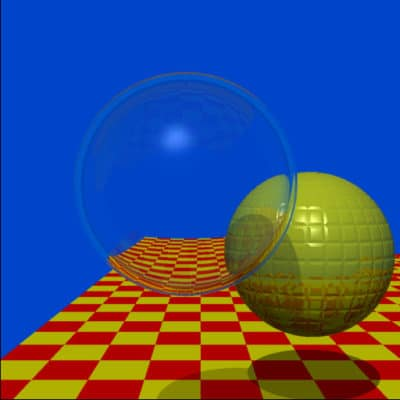
\includegraphics[width=0.5\textwidth]{pics/whitted.jpg}
	\caption{Algoritmul Ray Tracing recursiv, ilustrat de Turner Whitted\protect\footref{fn:whitted}}
	\label{fig:whitted}
\end{figure}

\subsection*{Ray Marching}\label{sec:raymarching}

Un algoritm foarte drag mie, datorită eleganței matematice, este Ray Marching.
Dacă celelalte metode de Ray Tracing calculează intersecții cu obiecte definite
prin primitive geometrice (e.g., triunghiuri), această variantă ia în considerare
doar suprafețe definite prin câmpuri de distanță (SDF). Un câmp de distanță este
o funcție asociată unei mulțimi care întoarce distanța ortogonală de la un punct
din spațiu la frontiera mulțimii. Un SDF are valori pozitive pentru puncte aflate
în afara mulțimii și valori negative pentru puncte aflate în interiorul mulțimii.
Principala caracteristică a acestui algoritm
care îl diferențiază de celelalte este faptul că nu calculează intersecții.
În schimb, fiecare rază mărșăluiește treptat în spațiu, apropiindu-se din ce în ce mai mult
de suprafețele definite, dar fără a le intersecta.
La fiecare pas, algoritmul se folosește de aceste câmpuri de distanță pentru a
calcula o rază minimă în jurul punctului curent, care reprezinte sfera de dimensiune
maximă care nu intersectează cu certitudine nicio suprafață. Această rază este
numită pas de marșăluire (marching step) și este folosită pentru a avansa
în spațiu. Algoritmul se oprește când distanța minimă calculată este mai mică
decât o anumită toleranță (indicând faptul că o intersecție este foarte aproape),
sau când un număr maxim de pași prestabilit este atins (caz în care nu se înregistrează nicio intersecție).
Datorită utilizării sferelor pentru mărșăluire, algoritmul mai este cunoscut și
sub numele de Sphere Tracing.
O ilustrație a funcționării acestuia se poate vedea în Figura~\ref{fig:raymarching}.

O aplicație naturală a acestui algoritm este randarea suprafețelor implicite.
Acestea sunt suprafețe în spațiul Euclidian definite prin ecuații de forma
\begin{equation}
	f(x, y, z) = 0.
\end{equation}
Funcția $f$ definește câmpul de distanță al suprafeței. De asemenea, se pot
calcula foarte ușor și vectorii normali la suprafață (gradientul funcției $f$),
ceea ce face posibilă randarea efectelor de iluminare a suprafețelor.
Exemple de randări ale unor suprafețe implicite se pot vedea în Figurile~\ref{fig:diffraction}
și~\ref{fig:fractal}.

Deși acest algoritm a fost studiat în literatura de specialitate încă din 1996 de către Hart~\cite{hart1996sphere},
el a devenit popular în cadrul demoscene-ului\footnote{\url{https://en.wikipedia.org/wiki/Demoscene}. Accesat 20.06.2024.}
și a comunității de programatori de shadere. Inigo Quilez a fost printre primii
care a adus algoritmul în atenția publicului larg, prin intermediul platformei
Shadertoy\footnote{\url{https://www.shadertoy.com/}. Accesat 20.06.2024.}
și a blogului personal\footnote{\url{https://iquilezles.org/}. Accesat 20.06.2024.}.


\begin{figure}[ht]
	\centering
	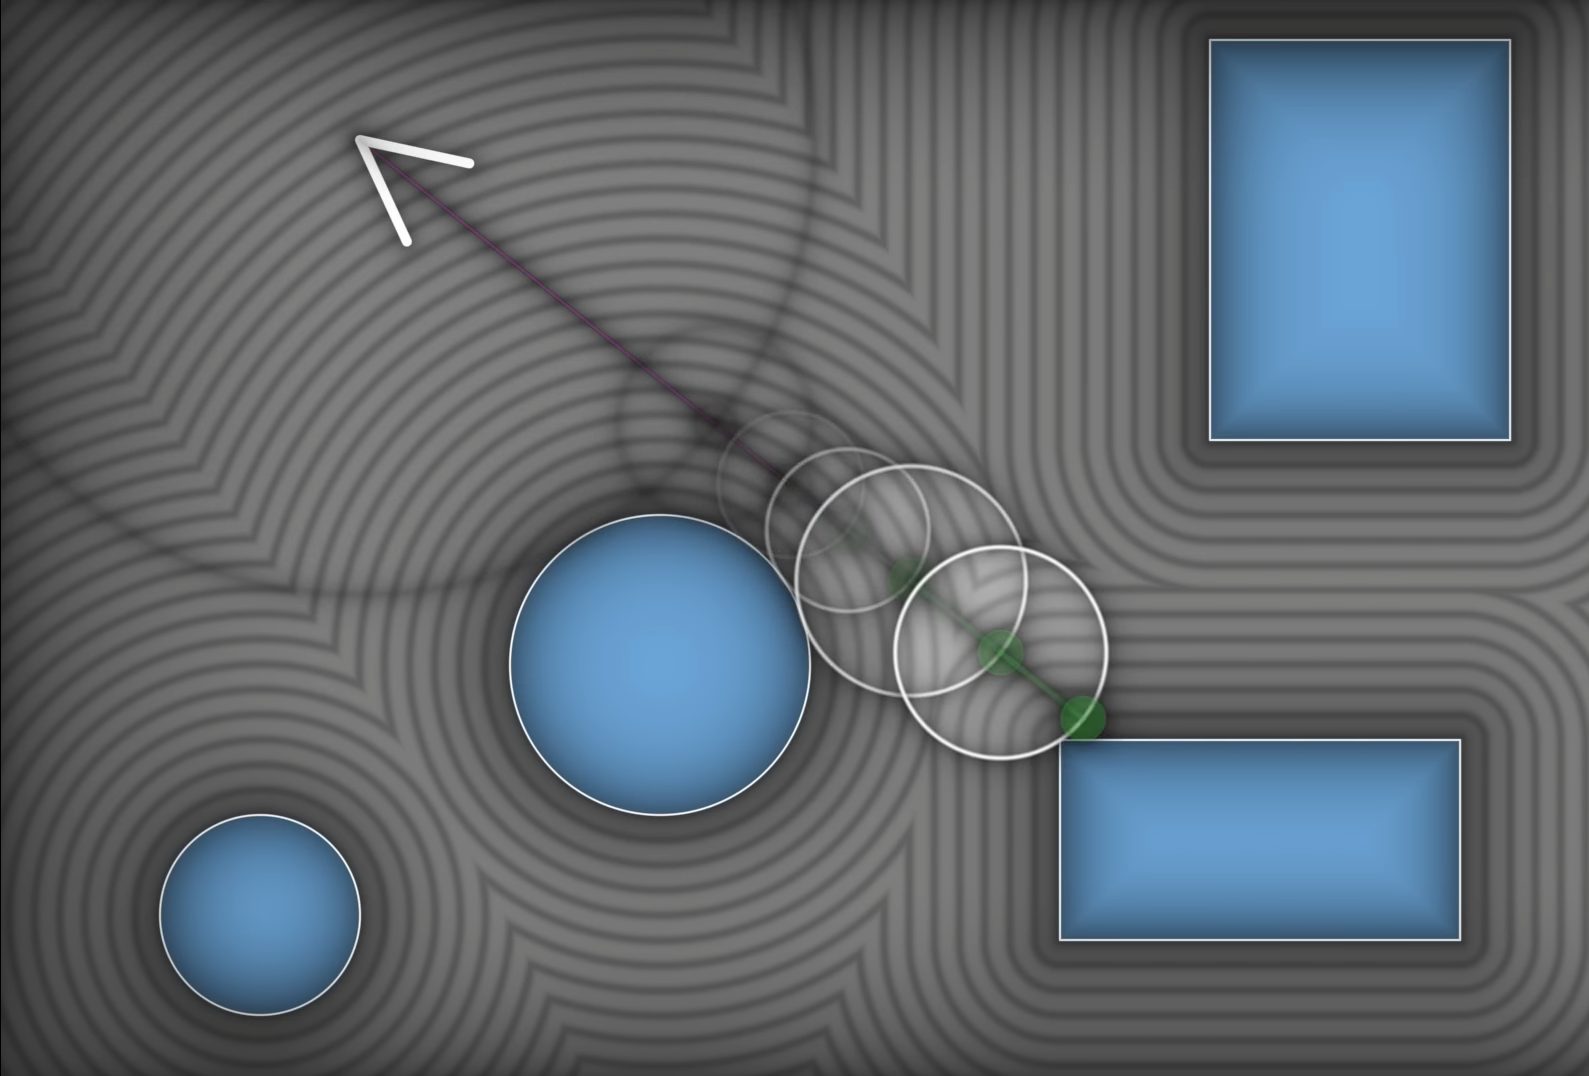
\includegraphics[width=0.7\textwidth]{pics/raymarching.png}
	\caption{Algoritmul Sphere Tracing - reprezentare 2D. Se pot observa și câmpurile de distanță ale obiectelor\protect\footnotemark}
	\label{fig:raymarching}
\end{figure}
\footnotetext{\copyright\url{https://www.youtube.com/@simondev758}. Accesat 20.06.2024.}

\begin{figure}[ht]
	\centering
	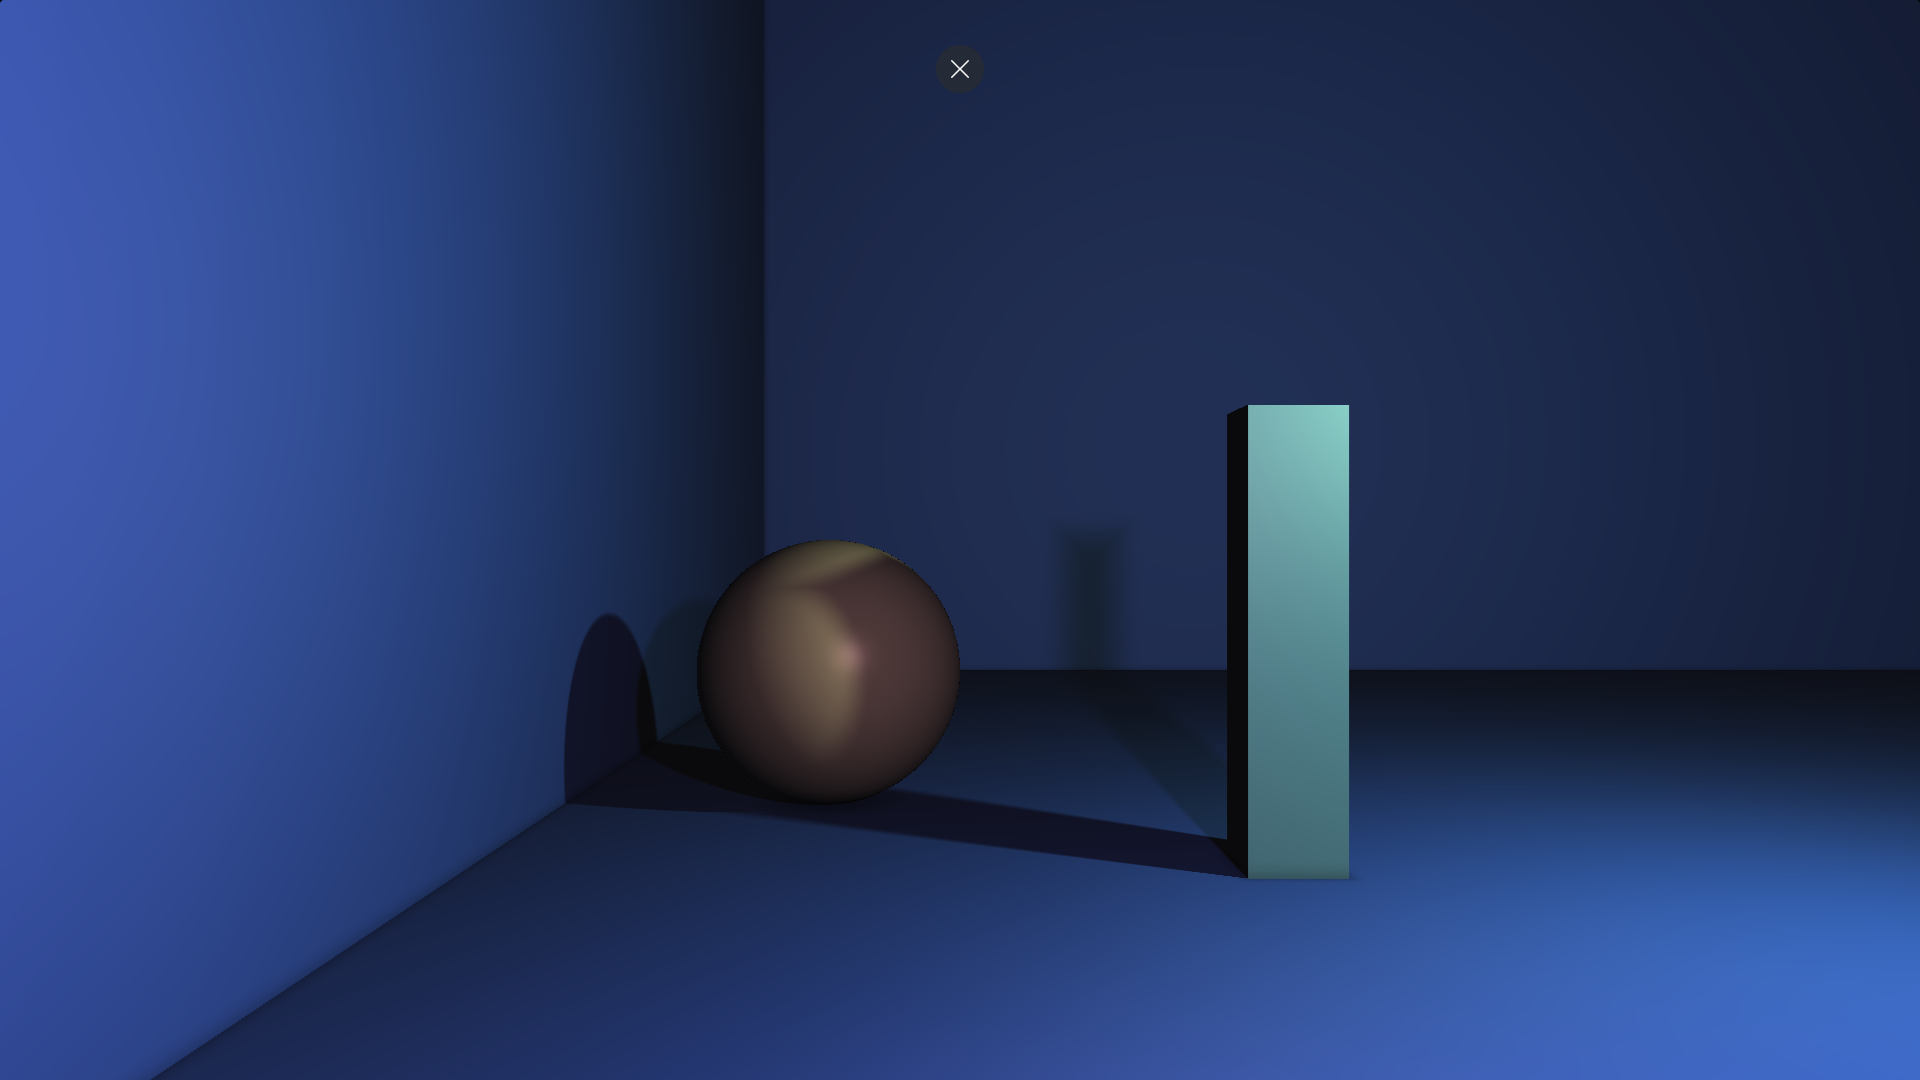
\includegraphics[width=0.7\textwidth]{pics/diffraction.png}
	\caption{Shader scris în GLSL care demonstrează soft shadows bazate pe difracție\protect\footnotemark}
	\label{fig:diffraction}
\end{figure}
\footnotetext{Shader scris de mine, disponibil la adresa: \url{https://www.shadertoy.com/view/tscSRS}. Accesat 20.06.2024.}

\begin{figure}[ht]
	\centering
	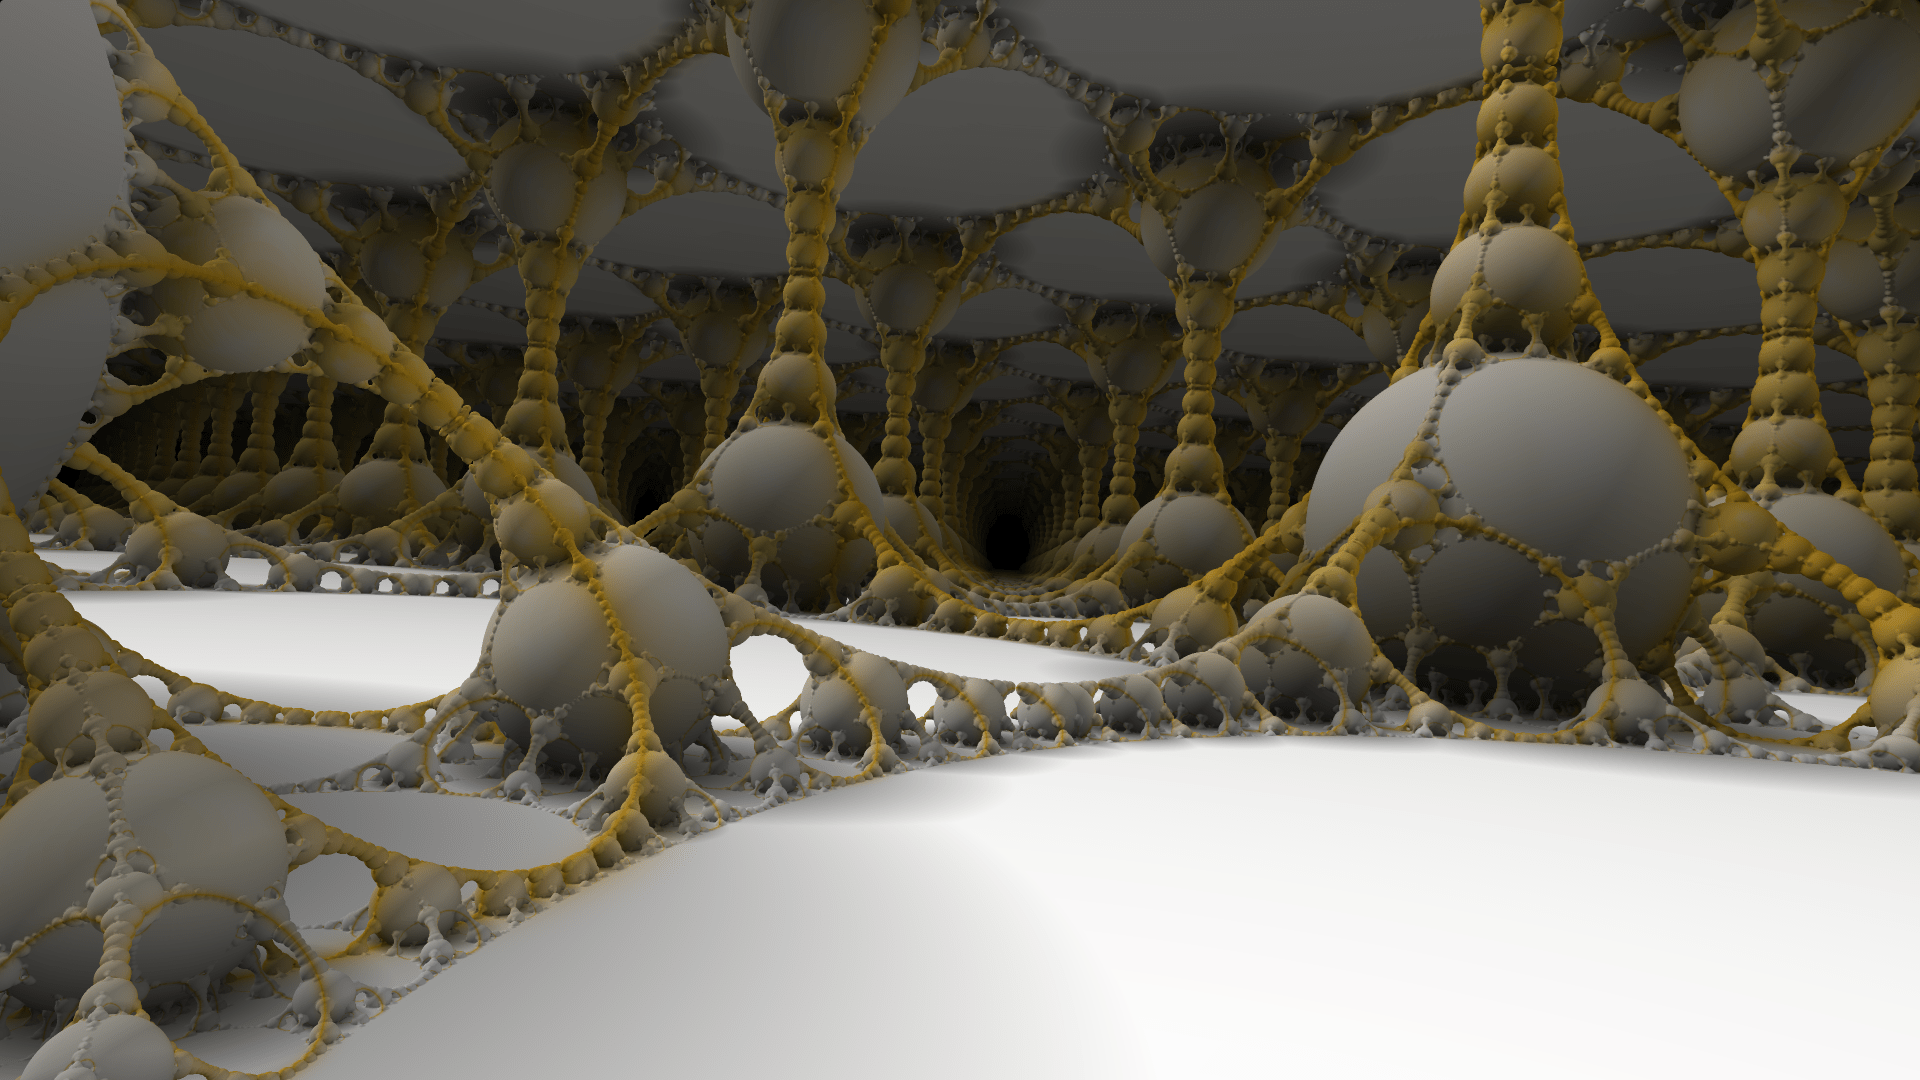
\includegraphics[width=0.7\textwidth]{pics/fractal.png}
	\caption{Randare 3D a unui fractal de tip Apollonian\protect\footnotemark}
	\label{fig:fractal}
\end{figure}
\footnotetext{\copyright Inigo Quilez: \url{https://www.shadertoy.com/view/4ds3zn}. Accesat 20.06.2024.}

\section{Metode Monte Carlo}

Algoritmii prezentați mai sus au pus bazele teoretice și practice pentru metode
mai avansate de randare, care se concentrează pe realism. Un dezavantaj major al
metodelor prezentate până acum este faptul că acestea nu sunt fotorealiste - ele
nu iau în considerare toate fenomenele interacțiunii luminii cu materialele. Deși
Ray Tracing recursiv poate calcula reflexii și refracții perfecte, acesta nu poate simula
din punct de vedere fizic efecte precum difuzia, dispersia, radianța, etc. Spre exemplu,
un obiect care nu este perfect reflectant sau refractant va difuza lumina în toate
direcțiile, nu doar în cea de reflexie sau refracție geometrică. De asemenea,
algoritmul de Ray Tracing recursiv consideră că lumina este o sursă punctiformă,
când de fapt aceasta are o distribuție finită în spațiu. Astfel, umbrele generate
de acest algoritm sunt "dure" și nu iau în considerare umbrele penumbrale. Este
adevărat că se pot aproxima aceste efecte folosind diferite modele de iluminare
care se aplică și în rasterizare (e.g., modelul Phong~\cite{Phong}),
dar acestea sunt doar aproximații și nu oferă realismul dorit.

Este nevoie așadar de modele mai avansate ale transportului luminii, care să
simuleze fenomenele fizice cu o acuratețe cât mai mare. Vom prezenta în continuare
metode care au la bază soluționarea ecuației de transport a luminii~\cite{Kajiya}
(folosind extensiv concepte din teoria probabilității), metode
care oferă o fidelitate net superioară celor prezentate anterior.
Pentru că scopul acestei lucrări nu este de a oferi o
introducere în teoria probabilității, vom prezenta doar conceptele de bază necesare
înțelegerii algoritmilor de tip Monte Carlo. Pentru o introducere mai detaliată în
acest domeniu, cititorul poate consulta lucrări de specialitate precum~\cite{Halton}
și~\cite{Hammersley}.

Metodele de tip Monte Carlo sunt metode
iterative care folosesc eșantionare aleatoare pentru a aproxima valoarea unei
integrale sau pentru a simula comportamentul unui sistem complex determinist,
modelat stocastic. Ele sunt utilizate pentru a găsi soluții aproximative, care
să conveargă către soluția corectă, pentru probleme intractabile sau care nu pot
fi rezolvate analitic.

Un exemplu de pași pe care îi urmează un algoritm de tip Monte Carlo este:
\begin{enumerate}
	\item Definirea unui domeniu de eșantionare
	\item Generarea unui număr de eșantioane în domeniu, folosind o distribuție de probabilitate
	\item Efectuarea calculelor (deterministe) pentru fiecare eșantion, care să aproximeze soluția
	\item Agregarea rezultatelor.
\end{enumerate}

\subsection{Integrare Monte Carlo}

Relevant în particular pentru această lucrare este conceptul de integrare Monte Carlo.
Acesta se referă la aproximarea unei integrale definite folosind metode Monte Carlo
de eșantionare.

Să luăm un exemplu de problemă. Dându-se o funcție $$f: \mathbb{D} \to \mathbb{R}$$
și o variabilă aleatoare continuă $X$ cu distribuția de probabilitate $p(x)$, vrem să calculăm
valoarea medie (expected value)
\begin{equation}\label{eq:expected_value}
	\mathbb{E}_p(f(X)) = \int_{\mathbb{D}} f(x) p(x)\diff x.
\end{equation}

Valoarea medie se poate aproxima prin eșantionare, folosind formula
\begin{equation}
	\mathbb{E}_p(f(X)) \approx \frac{1}{N} \sum_{i=1}^{N} f(x_i),
\end{equation}
aproximarea devenind mai bună cu creșterea numărului de eșantioane $N$.

Așadar, putem aproxima integrala~(\ref{eq:expected_value}) prin
\begin{equation}\label{eq:estimator}
	\int_{\mathbb{D}} f(x) p(x)\diff x \approx \frac{1}{N} \sum_{i=1}^{N} f(x_i).
\end{equation}

Partea dreaptă a ecuației~(\ref{eq:estimator}) este estimatorul Monte Carlo.
Teorema limitei centrale afirmă că, pentru un număr suficient de mare de eșantioane,
distribuția de probabilitate a estimărilor se apropie de o distribuție normală în
jurul valorii medii estimate. Acest lucru înseamnă că estimatorul Monte
Carlo este imparțial (unbiased) și are o varianță redusă. Dacă notăm cu $f_p$
estimatorul, atunci au loc următoarele relații:
\begin{equation}
	\begin{aligned}
		\mathbb{E}_p(f_p) & = \mathbb{E}_p(f(X)),     \\
		Var_p(f_p)        & = \frac{1}{N}Var_p(f(X)).
	\end{aligned}
\end{equation}

\subsection{Eșantionare bazată pe importanță}\label{sec:is}

În practică, distribuția de probabilitate $p(x)$ este adesea greu de eșantionat,
sau nu produce varianța cea mai mică, ceea ce duce la o convergență lentă a
estimării.
Eșantionarea pe baza importanței (importance sampling) este o tehnică prin care
se eșantionează variabila aleatoare $X$ dintr-o altă distribuție de probabilitate,
$q(x)$, cu scopul de a reduce varianța și a estima mai bine valoarea medie a funcției
$f$.

Să introducem această distribuție în ecuația valorii medii~(\ref{eq:expected_value}):
\begin{equation}
	\begin{aligned}
		\mathbb{E}_p(f(X)) & = \int_{\mathbb{D}} f(x) p(x)\diff x                   \\
		                   & = \int_{\mathbb{D}} f(x) \frac{p(x)}{q(x)} q(x)\diff x \\
		                   & = \mathbb{E}_q\left(f(X) \frac{p(X)}{q(X)}\right).
	\end{aligned}
\end{equation}

Obținem astfel un nou estimator Monte Carlo, notat cu $f_q$, care își păstrează imparțialitatea
(căci valoarea medie rămâne aceeași) și care folosește distribuția $q(x)$:
\begin{equation}
	\mathbb{E}_q(f_q) = \mathbb{E}_p(f(X)) \approx \frac{1}{N} \sum_{i=1}^{N} f(x_i) \frac{p(x_i)}{q(x_i)}.
\end{equation}

Varianța acestui estimator, este dată de
\begin{equation}
	Var_q(f_q) = \frac{1}{N}Var_q\left(f(X) \frac{p(X)}{q(X)}\right).
\end{equation}

Scopul este de a alege distribuția $q(x)$ astfel încât varianța estimatorului să fie
mai mică decât varianța inițială, i.e.
\begin{equation}
	\frac{1}{N}Var_q\left(f(X) \frac{p(X)}{q(X)}\right) < \frac{1}{N}Var_p(f(X)).
\end{equation}

Pentru a minimiza varianța noului estimator, în mod ideal, vrem ca funcția
$f(x) \dfrac{p(x)}{q(x)}$ să fie constantă, pentru orice $x$ eșantionat, ceea
ce ar duce la o varianță nulă. Acest lucru se întamplă dacă
\begin{equation}\label{eq:optimal_q}
	q(x) = c \cdot f(x)p(x),
\end{equation}
unde $c$ este o constantă de normalizare. Pentru a păstra imparțialitatea, $c$ trebuie
să fie egal cu $\dfrac{1}{\mathbb{E}_p(f(X))}$, însă această valoare este necunoscută
(altfel nu am mai avea nevoie de estimator!). Așadar, nu este fezabilă alegerea
optimă pentru $q(x)$. Totuși, ecuația~(\ref{eq:optimal_q}) ne arată că distribuția
optimă este proporțională cu funcția $f(x)p(x)$. Acest produs măsoară fix
importanța fiecărui eșantion în estimarea mediei, de unde și numele tehnicii.

În Figura~\ref{fig:is} se poate observa efectul eșantionării bazate pe importanță.
În acest caz, funcția $f$ are o regiune mică de unde vine majoritatea contribuției
către valoarea medie. Dacă distribuția de probabilitate $p$ nu eșantionează bine
această regiune (în acest caz, este o distribuție uniformă), varianța estimării
va fi mare. Distribuția $q$ este aleasă astfel încât să eșantioneze mai mult din
zonele importante și se poate vedea pe subgraficul din dreapta cum raportul
$\dfrac{p(x)}{q(x)}$ încearcă să echilibreze contribuția fiecărui eșantion, reducând
varianța estimării.

\begin{figure}[th]
	\centering
	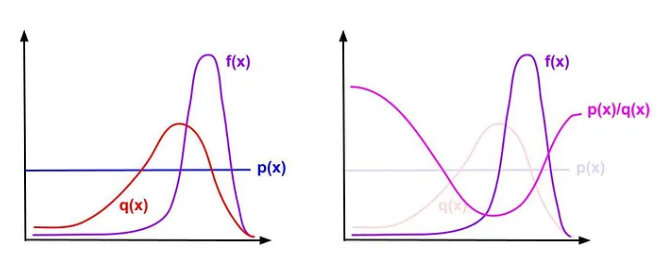
\includegraphics[width=\textwidth]{pics/is.png}
	\caption{Efectul eșantionării bazate pe importanță\protect\footnotemark}
	\label{fig:is}
\end{figure}
\footnotetext{\copyright\url{https://medium.com/}}

\subsection{Eșantionare Stratificată}\label{sec:stratified}

O altă metodă de a reduce varianța estimării este eșantionarea stratificată (Stratified Sampling).
În această metodă se partiționează domeniul de eșantionare $\mathbb{D}$ în $n$ subdomenii,
numite straturi, iar evaluarea integralei se face pe fiecare strat în parte:
\begin{equation}
	\int_{\mathbb{D}} f(x) p(x)\diff x = \sum_{i=1}^{n} \int_{\mathbb{D}_i} f(x) p(x)\diff x.
\end{equation}

În acest caz, varianța estimării devine suma varianțelor pe fiecare strat:
\begin{equation}
	Var(f_s) = \sum_{i=1}^{n} Var(f_i).
\end{equation}

Se poate demonstra că, în cazul în care toate straturile au aceeași măsură, i.e.
\begin{equation}
	\int_{\mathbb{D}_i} p(x)\diff x = \frac{1}{n}\int_{\mathbb{D}} p(x)\diff x, \quad \forall i \in \{1, 2, \ldots, n\},
\end{equation}
atunci varianța estimării nu va fi mai mare decât fără eșantionare stratificată.
Pentru mai multe informații se poate consulta cartea de specialitate a lui Kleijnen et al.~\cite{Kleijnen2013}.

Un exemplu de eșantionare stratificată este ilustrat sub tehnica de jittering
în eșantionarea pixelilor, detaliată în capitolul~\ref{sec:implementare}.

\subsection{Ecuația transportului luminii}

Introdusă simultan de Kajiya~\cite{Kajiya} și Immel et al.~\cite{Immel} în 1986,
ecuația transportului luminii (sau ecuația de randare) este cea mai importantă ecuație din domeniul
graficii pe calculator. Aceasta descrie modul în care lumina interacționează
cu suprafețele și ajunge către observator. Una dintre formele acesteia este:
\begin{equation}
	\label{eq:light_transport}
	\begin{aligned}
		L_o(\mathbf{x}, \omega_o, \lambda, t) & = L_e(\mathbf{x}, \omega_o, \lambda, t) + L_r(\mathbf{x}, \omega_o, \lambda, t)                                                                     \\
		L_r(\mathbf{x}, \omega_o, \lambda, t) & = \int_{\Omega_+} f_r(\mathbf{x}, \omega_i, \omega_o, \lambda, t) L_i(\mathbf{x}, \omega_i, \lambda, t) (\omega_i \cdot \mathbf{n}) \diff \omega_i.
	\end{aligned}
\end{equation}

Sunt destul de multe simboluri folosite în această ecuație, așa că le vom explica
pe rând. Folosind Figura~\ref{fig:light_transport2} drept referință:
\begin{itemize}
	\item $\mathbf{x}$ este poziția punctului de intersecție cu suprafața
	\item $\omega_o$ este direcția de observare (direcția pe care vrem să măsurăm radianța)
	\item $\omega_i$ este opusul direcției de incidență (direcționat de la punctul de intersecție către sursa de lumină)
	\item $\mathbf{n}$ este normala la suprafață în punctul $\mathbf{x}$
	\item $\lambda$ este lungimea de undă a luminii
	\item $t$ este un moment particular în timp
	\item $L_o(\mathbf{x}, \omega_o, \lambda, t)$ este radianța spectrală de lungime de undă $\lambda$ observată în punctul $\mathbf{x}$, pe direcția $\omega_o$, la momentul $t$
	\item $L_e(\mathbf{x}, \omega_o, \lambda, t)$ este radianța spectrală de lungime de undă $\lambda$ emisă de suprafața în punctul $\mathbf{x}$, pe direcția $\omega_o$, la momentul $t$
	\item $L_r(\mathbf{x}, \omega_o, \lambda, t)$ este radianța spectrală de lungime de undă $\lambda$ reflectată în punctul $\mathbf{x}$, pe direcția $\omega_o$, la momentul $t$
	\item $L_i(\mathbf{x}, \omega_i, \lambda, t)$ este radianța spectrală de lungime de undă $\lambda$ incidentă în punctul $\mathbf{x}$, pe direcția $\omega_i$, la momentul $t$
	\item $f_r(\mathbf{x}, \omega_i, \omega_o, \lambda, t)$ este funcția de distribuție bidirecțională a reflectanței (BRDF), care reprezintă câtă lumină este reflectată în direcția $\omega_o$ din direcția $\omega_i$
	\item $\Omega_+$ este emisfera unitate superioară centrată în jurul normalei $\mathbf{n}$, care conține toate direcțiile posibile de incidență $\omega_i$ pentru care $\omega_i \cdot \mathbf{n} > 0$.
\end{itemize}

Putem observa că această ecuație nu include o componentă de transmisie a luminii.
Putem augmenta aditiv ecuația~\ref{eq:light_transport} cu o componentă de transmisie, definită astfel:
\begin{equation}
	L_t(\mathbf{x}, \omega_o, \lambda, t) = \int_{\Omega_-} f_t(\mathbf{x}, \omega_t, \omega_o, \lambda, t) L_i(\mathbf{x}, \omega_t, \lambda, t) (\omega_t \cdot \mathbf{n}) \diff \omega_i,
\end{equation}
cu diferența că $\Omega_-$ este emisfera unitate inferioară centrată în jurul normalei $\mathbf{n}$, care conține toate direcțiile posibile de incidență internă $\omega_t$ pentru care $\omega_t \cdot \mathbf{n} < 0$.
În acest caz, funcția $f_t(\mathbf{x}, \omega_t, \omega_o, \lambda, t)$ este funcția de distribuție bidirecțională a transmisiei (BTDF), care reprezintă câtă lumină este transmisă în direcția $\omega_o$ din direcția $\omega_t$.

De obicei, componenta de reflectanță și cea de transmisie se combină într-o singură
componentă, care are la bază o funcție de distribuție bidirecțională a împrăștierii (BSDF).
Mai multe detalii despre această clasă de funcții, într-un context de materiale
bazate pe fizică, se pot găsi în secțiunea~\ref{sec:pbr}.

\begin{figure}[ht]
	\centering
	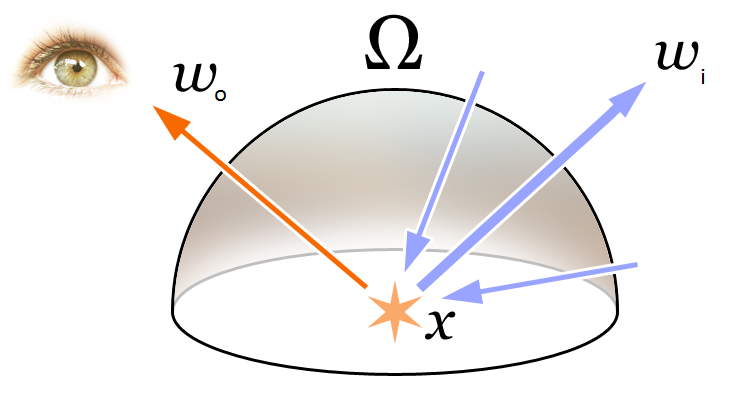
\includegraphics[width=0.5\textwidth]{pics/rendering_eq2.png}
	\caption{Ilustrație a componentelor din ecuația de randare\protect\footref{fn:wiki}}
	\label{fig:light_transport2}
\end{figure}

\begin{figure}[ht]
	\centering
	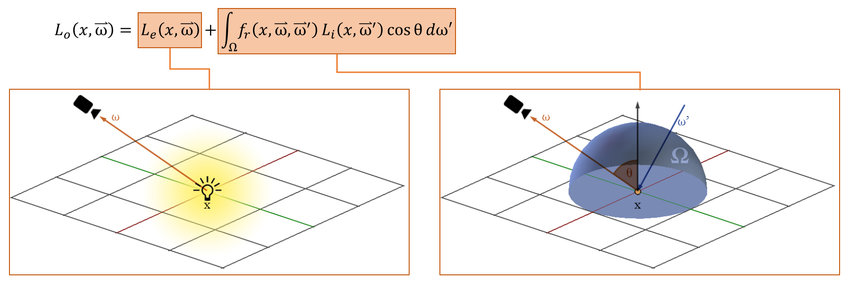
\includegraphics[width=0.8\textwidth]{pics/rendering_eq.png}
	\caption{Formă alternativă a ecuației transportului luminii. Se pot vedea componentele de emisie și împrăștiere\protect\footnotemark}
	\label{fig:light_transport}
\end{figure}
\footnotetext{\copyright\url{https://www.researchgate.net/}. Accesat 20.06.2024.}

Găsirea soluției la ecuația transportului luminii (i.e., determinarea radianței $L_o$)
este provocarea primară în algoritmii de randare realistică. Vom enumera în secțiunea următoare câteva dintre
metodele de rezolvare a acestei ecuații, însă ne vom concentra asupra algoritmului
de Path Tracing.


\section{Radiosity}\label{sec:radiosity}
Radiosity este o tehnică de iluminare globală bazată pe metoda elementului finit.
Aceasta presupune împărțirea scenei în elemente mici, numite petice, și calcularea
energiei luminoase reflectată de fiecare dintre acestea. Algoritmul în sine consideră
numai interacțiunile de tip difuz, ceea ce îl face să fie un algoritm independent
de direcția de vizualizare. De aceea, acesta poate fi folosit în special pentru a precalcula
iluminarea statică a scenei (spre exemplu, la compilarea unei hărți create în editorul
Hammer al companiei Valve se aplică acest algoritm sub forma utilitarului VRAD\footnote{\url{https://developer.valvesoftware.com/wiki/VRAD}. Accesat 20.06.2024.}).

Algoritmul funcționează prin calcularea vizibilității între petice și asocierea
unori factori de vizualizare pentru fiecare pereche. Acest factor descrie
cât de bine se văd două petice între ele.

Într-o variantă brută a algoritmului, factorii sunt folosiți drept coeficienți pentru a rezolva
un sistem de ecuații liniare (unde ecuațiile sunt variante simplificate ale ecuației
de transport al luminii). Soluția acestui sistem oferă radiozitatea fiecărui petice
(i.e., luminozitatea). O ilustrație a rezultatului algoritmului într-o scenă
de tip Cornell Box se poate vedea în Figura~\ref{fig:radiosity}.

O variantă optimizată, denumită "shooting radiosity", folosește un proces iterativ în
care la fiecare pas se emite lumină dintr-un petice și se calculează radianța
reflectată de celelalte petice. Acest proces se repetă până când se atinge o stare
stabilă, așa cum se poate vedea în Figura~\ref{fig:shooting_radiosity}.

Avantajele algoritmului sunt faptul că este relativ simplu de implementat, nu necesită
matematică avansată și deci este un instrument didactic bun. De asemenea, caracterul
său independent de direcție îl face potrivit pentru precalcularea iluminării statice.
Ca dezavantaje, este un algoritm lent și trebuie făcut un compromis între timpul de
randare și calitatea rezultatului (e.g., rezoluția peticelor, numărul de pași). Nu este
potrivit pentru iluminarea speculară sau transmisie, fiind limitat la interacțiuni de tip difuz
(deși poate fi extins la medii non-difuze~\cite{Immel}).
Un alt aspect care îl limitează este nevoia de a precalcula funcția de vizibilitate între petice.
Din experiență proprie, lucrând la hărți complexe în editorul Hammer\footnote{\url{https://developer.valvesoftware.com/wiki/Valve_Hammer_Editor}. Accesat 20.06.2024.},
era necesar să ajut manual algoritmul de radiosity prin partiționarea artificială a
scenei în zone de vizibilitate\footnote{\url{https://developer.valvesoftware.com/wiki/VIS_optimization}. Accesat 20.06.2024.}, pentru a reduce numărul de perechi de petice care
trebuiau luate în considerare. Fără această intervenție, doar calculul vizibilității\footnote{\url{https://developer.valvesoftware.com/wiki/VVIS}. Accesat 20.06.2024.}
putea să dureze și 24 de ore.

\begin{figure}[ht]
	\centering
	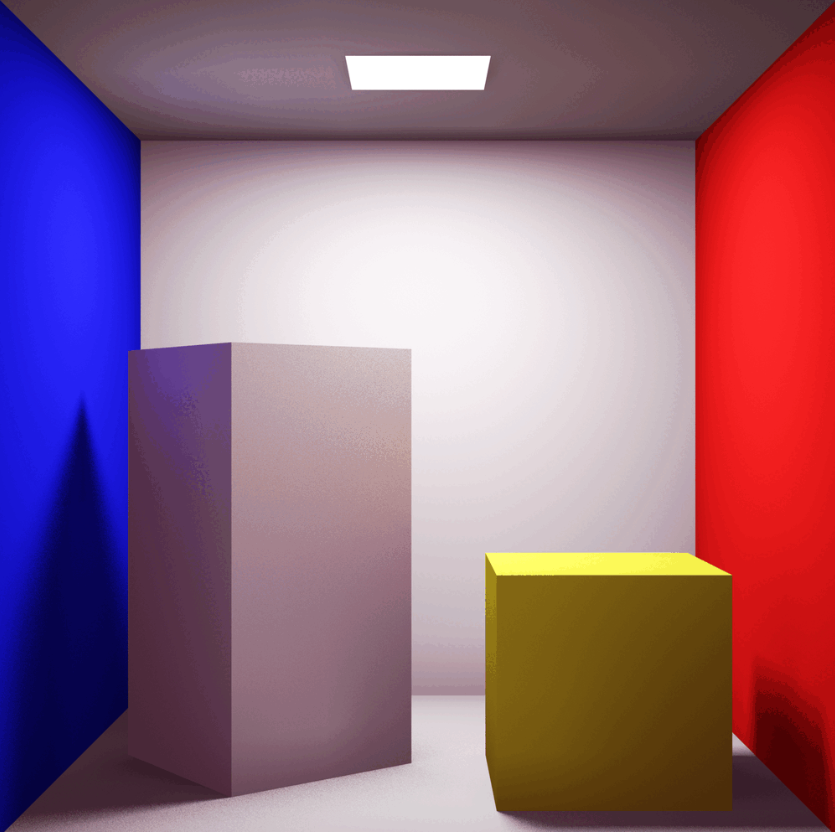
\includegraphics[width=0.5\textwidth]{pics/radiosity.png}
	\caption{Rezultatul algoritmului de radiosity într-o scenă de tip Cornell Box\protect\footref{fn:wiki}}
	\label{fig:radiosity}
\end{figure}
\begin{figure}[ht]
	\centering
	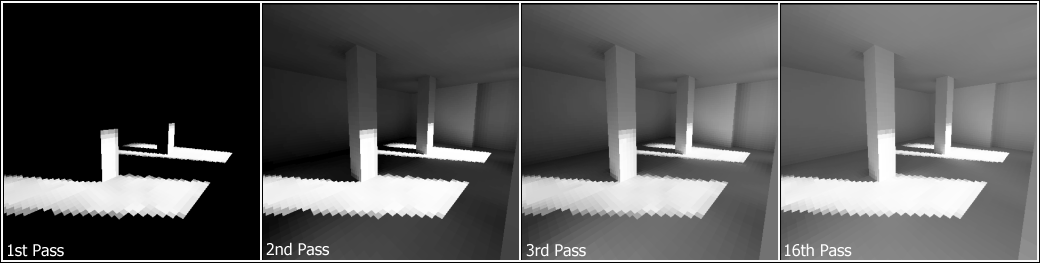
\includegraphics[width=0.8\textwidth]{pics/shooting_radiosity.png}
	\caption{Ilustrație a algoritmului de shooting radiosity. Tot aici se poate observa și rezoluția peticelor\protect\footref{fn:wiki}}
	\label{fig:shooting_radiosity}
\end{figure}

\section{Path Tracing}\label{sec:path_tracing}

Algoritmul Radiosity face o presupunere simplificatoare, și anume că iluminarea
venită de pe suprafețe depinde doar de direcția de ieșire, și nu și de direcția
incidentă. Vedem totuși că ecuația transportului luminii~(\ref{eq:light_transport})
include un termen de distribuție $f$ care depinde de ambele direcții (de unde
și numele de distribuție bidirecțională). Algoritmul de Path Tracing modelează
acest aspect, ajustând probabilistic contribuția fiecărui eșantion la radianța
observată.

O variantă naivă a algoritmului este prezentată în Pseudocodul~\ref{alg:path_tracing}.
Dacă ar fi să sumarizăm pașii algoritmului, aceștia ar fi:
\begin{enumerate}
	\item Pentru fiecare pixel din imagine: \label{enum:pt1}
	      \begin{enumerate}
		      \item Generăm o rază de la observator către pixel
		      \item Intersectăm raza cu scena
		      \item Dacă nu există intersecție, pixelul primește culoarea de fundal și ne întoarcem la pasul~\ref{enum:pt1}
		      \item Altfel, calculăm contribuția de lumină pentru punctul intersectat (folosind BRDF)
		      \item Eșantionăm o nouă rază pornind din punctul intersectat, în funcție de BRDF
		      \item Calculăm contribuția de lumină pentru noua rază, recursiv
	      \end{enumerate}
	\item În final, mediem contribuțiile pentru a obține culoarea pixelului.
\end{enumerate}

\begin{algorithm}[H]
	\caption{Pseudocodul algoritmului de Path Tracing recursiv}\label{alg:path_tracing}
	\begin{algorithmic}[1]
		\Function{PathTrace}{$ray, depth$}
		\If{$depth > MAX\_DEPTH$}
		\State \Return $backgroundColor$	\Comment{Ne oprim dacă am atins adâncimea maximă}
		\EndIf
		\State $intersection \gets$ \Call{IntersectScene}{$ray$} \Comment{Intersectăm raza cu scena}
		\If{$intersection = \texttt{null}$}
		\State \Return $backgroundColor$	\Comment{Ne oprim dacă nu există intersecție}
		\EndIf
		\State $m \gets intersection.material$
		\State $p \gets intersection.position$
		\State $n \gets intersection.normal$
		\State $v \gets -ray.direction$
		\State $bounceRay \gets$ \Call{SampleRay}{$m, p, n$}	\Comment{Eșantionăm o nouă rază}
		\State $pdf \gets$ \Call{Pdf}{$m, n, bounceRay$}		\Comment{Evaluăm probabilitatea de eșantionare}
		\State $reflectance \gets$ \Call{EvalBRDF}{$m, n, v, bounceRay$} \Comment{Evaluăm reflectanța}
		\State $color \gets$ \Call{PathTrace}{$bounceRay, depth + 1$}	 \Comment{Pasul recursiv}
		\State \Return $m.emission + reflectance \cdot color / pdf$		 \Comment{Evaluăm ecuația de rendering}
		\EndFunction
		\Function{Render}{$pixels, samples$}
		\For {$p$ in $pixels$}
		\For {$i \gets 1$ to $samples$}
		\State $ray \gets$ \Call{GenerateCameraRay}{$p, i$}	\Comment{Generăm raza de la observator}
		\State $pixel.color \gets pixel.color + $ \Call{PathTrace}{$ray, 0$}	\Comment{Acumulăm contribuția}
		\EndFor
		\State $pixel.color \gets pixel.color / samples$ \Comment{Mediem contribuțiile}
		\EndFor
		\EndFunction

	\end{algorithmic}
\end{algorithm}

Algoritmul Path Tracing reprezintă transpunerea completă a ecuației de randare
într-un algoritm de calcul numeric. Se poate cupla orice tip de BRDF la acest
algoritm, ceea ce îl face extrem de versatil. Se pot obține simulări de interacțiuni
difuze (precum cele obținute cu Radiosity), folosind un BRDF Lambertian~\cite{Lambert}, sau
simulări de interacțiuni speculare, folosind un BRDF precum Cook-Torrance(\cite{CookTorrance}).
Se poate extinde de asemenea și la interacțiuni de transmisie, folosind un BTDF.
Path Tracing este o metodă generală de rezolvare a ecuației de randare, iar componentele
sale pot fi alese în funcție de necesități. Identificăm astfel câteva dintre diferitele
categorii de strategii de bază care pot fi customizate în Path Tracing.

\subsection{Strategii de eșantionare a pixelilor}

Pentru o convergență mai rapidă și o imagine mai stabilă, se rulează algoritmul
de mai multe ori pe același pixel și se combină rezultatele. Strategia de alegere
a eșantioanelor aferente unui pixel poate influența calitatea finală a imaginii.

Pentru vizualizare, să considerăm un sistem de 64 de eșantioane per pixel.
Cele mai comune opțiuni sunt:
\begin{itemize}
	\item Eșantionare uniformă (Figura~\ref{fig:uniform_sampling}): se alege același eșantion de fiecare dată
	\item Eșantionare stratificată uniformă (Figura~\ref{fig:uniform_sampling}): se împarte fiecare pixel în subpixeli și se alege câte un eșantion pentru fiecare subpixel
	\item Eșantionare aleatoare/jittering (Figura~\ref{fig:random_sampling}): fiecare eșantion este ales aleator
	\item Eșantionare stratificată + jittering (Figura~\ref{fig:random_sampling}): se împarte fiecare pixel în subpixeli și se alege un eșantion aleator pentru fiecare subpixel,
	      fără a se suprapune zonele de eșantionare.
\end{itemize}
\begin{figure}[ht]
	\centering
	\begin{subfigure}[h]{0.45\linewidth}
		\centering
		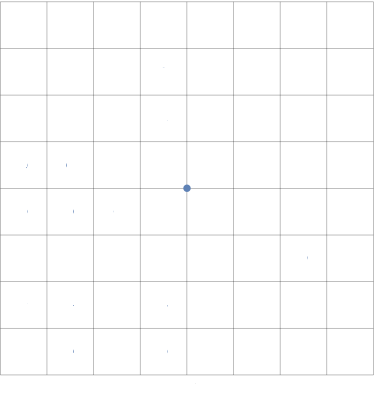
\includegraphics[width=\linewidth]{pics/point-samples.png}
		\caption{Eșantionare uniformă}
	\end{subfigure}
	\hfill
	\begin{subfigure}[h]{0.45\linewidth}
		\centering
		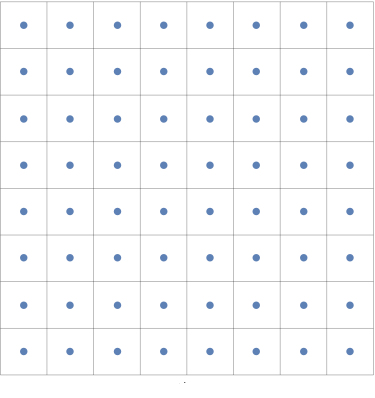
\includegraphics[width=\linewidth]{pics/uniform-point-samples.png}
		\caption{Eșantionare stratificată}
	\end{subfigure}
	\caption{Eșantionare uniformă vs stratificată\protect\footnotemark}
	\label{fig:uniform_sampling}
\end{figure}
\footnotetext{\label{pbr-book}\copyright\url{https://pbr-book.org/}. Accesat 20.06.2024.}
\begin{figure}[ht]
	\centering
	\begin{subfigure}[h]{0.45\linewidth}
		\centering
		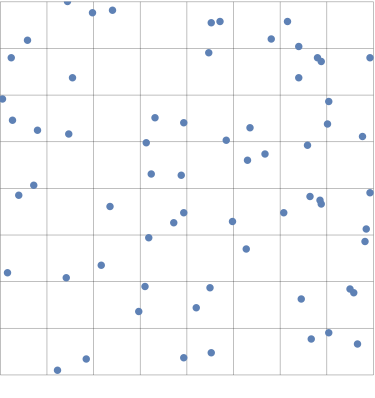
\includegraphics[width=\linewidth]{pics/random-point-samples.png}
		\caption{Eșantionare aleatoare}
	\end{subfigure}
	\hfill
	\begin{subfigure}[h]{0.45\linewidth}
		\centering
		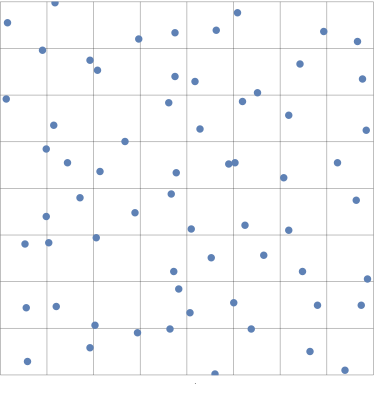
\includegraphics[width=\linewidth]{pics/jittered-point-samples.png}
		\caption{Eșantionare stratificată + jittering}
	\end{subfigure}
	\caption{Eșantionare aleatoare vs stratificată + jittering\protect\footref{pbr-book}}
	\label{fig:random_sampling}
\end{figure}

În mod evident, eșantionarea uniformă lasă multe de dorit. Aceasta produce artefacte
de tip aliasing în jurul obiectelor (Figura~\ref{fig:uniform_aliasing}). Eșantionarea
stratificată (descrisă și în secțiunea~\ref{sec:stratified}) reușește să rezolve parțial
această problemă, având date din mai multe zone ale pixelului. Eșantionarea aleatoare
este altă soluție la problema aliasing-ului, însă introduce prea mult zgomot. Totuși,
reușește să integreze mai bine semnalele de frecvență mare, cum ar fi cazul de randare
a unei texturi sub unghi mare.
Cea mai bună variantă este o combinație între cele două din urmă, care să ofere
avantaje din ambele părți. Comparații calitative sunt reprezentate în Figurile~\ref{fig:uniform_aliasing} și~\ref{fig:sampling_aliasing}.
\begin{figure}[ht]
	\centering
	\begin{subfigure}[h]{0.45\linewidth}
		\centering
		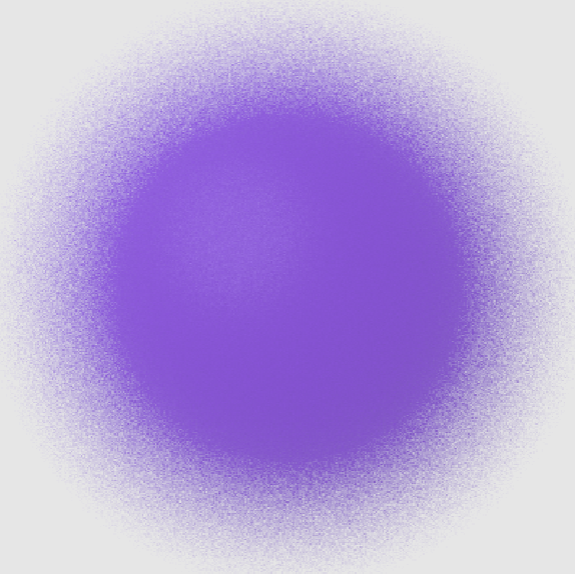
\includegraphics[width=\linewidth]{pics/random-circle.png}
		\caption{Eșantionare aleatoare}
	\end{subfigure}
	\hfill
	\begin{subfigure}[h]{0.45\linewidth}
		\centering
		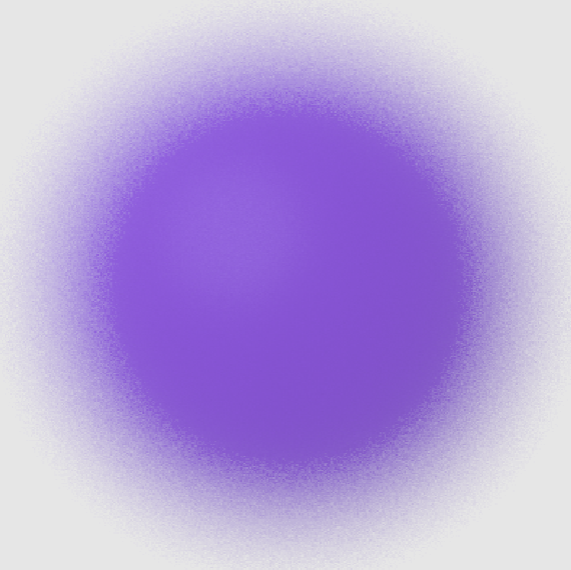
\includegraphics[width=\linewidth]{pics/stratified-circle.png}
		\caption{Eșantionare stratificată}
	\end{subfigure}
	\caption{Comparație la 1 eșantion per pixel. Se pot observa artefacte de aliasing în varianta de jittering\protect\footref{pbr-book}}
	\label{fig:uniform_aliasing}
\end{figure}
\begin{figure}[ht]
	\centering
	\begin{subfigure}[h]{0.7\linewidth}
		\centering
		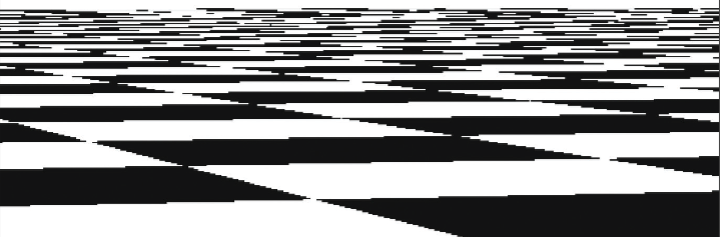
\includegraphics[width=\linewidth]{pics/uniform-checkerboard.png}
		\caption{Eșantionare stratificată}
	\end{subfigure}
	\hfill
	\begin{subfigure}[h]{0.7\linewidth}
		\centering
		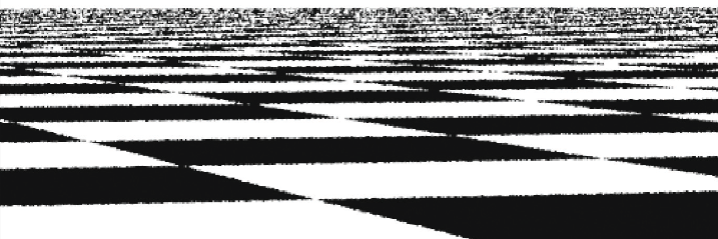
\includegraphics[width=\linewidth]{pics/jittered-checkerboard.png}
		\caption{Eșantionare aleatoare}
	\end{subfigure}
	\caption{Comparație la 1 eșantion per pixel. Varianta cu jittering minimizează artefactele dar adaugă zgomot\protect\footref{pbr-book}}
	\label{fig:sampling_aliasing}
\end{figure}

\subsection{\label{sec:pbr}Strategii de alegere a funcției de distribuție a reflectanței}

Un model bun de material (mai ales PBR) face diferența între o randare fotorealistă
și una care nu este. Chiar dacă algoritmul converge către soluția ecuației de transport,
rezultatul poate fi unul nerealist dacă nu se folosește un model de materiale adecvat.

\subsubsection*{BRDF}

Definit prima oară de un model matematic general de către Nicodemus (1965)~\cite{Nicodemus},
BRDF-ul este o funcție care descrie câtă lumină este reflectată într-o anumită direcție.
Am menționat-o de multe ori în cadrul acestei lucrări și am vorbit despre rolul
ei în cadrul ecuației de randare (atât de importantă este),
dar nu am explicat cum se construiește. Să considerăm modelul simplificat
în care nu se ține cont de lungimea de undă a luminii și nici de variabila de timp.
În acest caz, tot ce ne mai rămâne de făcut pentru a defini BRDF sunt două concepte
de radiometrie, pe care le vom defini informal aici:

\begin{definition}
	Radianța $L$ este măsura fluxului de lumină care trece printr-o suprafață unitară într-o direcție dată.
\end{definition}
\begin{definition}
	Iradianța $E$ este măsura fluxului de lumină primit de o suprafață unitară (din toate direcțiile).
\end{definition}

Așadar, observăm că radianța depinde de direcția incidentă, în timp ce iradianța
nu. O ilustrație a acestor concepte se poate vedea în Figura~\ref{fig:radiance}.
\begin{figure}[ht]
	\centering
	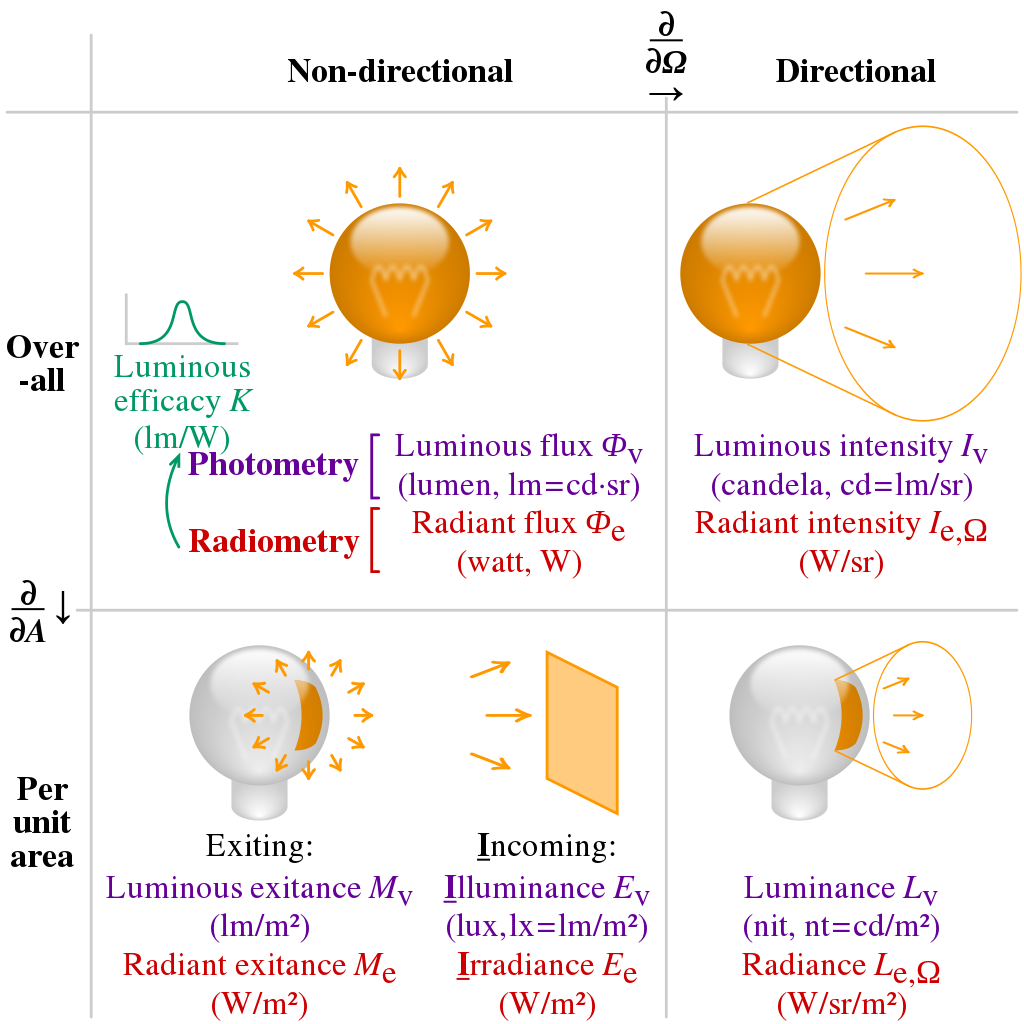
\includegraphics[width=0.5\textwidth]{pics/radiometry.png}
	\caption{Ilustrație a diferitelor mărimi fizice din radiometrie\protect\footref{fn:wiki}}
	\label{fig:radiance}
\end{figure}

Putem acum să definim, informal, BRDF-ul:
\begin{definition}
	Funcția de distribuție bidirecțională a reflectanței (BRDF) este raportul infinitezimal
	dintre radianța reflectată și iradianța incidentă, în funcție de direcția de incidență și de cea de reflexie.
\end{definition}
Matematic, aceasta se scrie sub forma:
\begin{equation}
	f_r(\mathbf{x}, \omega_i, \omega_o) = \frac{\diff L_r(\mathbf{x}, \omega_o)}{\diff E_i(\mathbf{x}, \omega_i)},
\end{equation}
Derivarea se face după direcția incidentă $\omega_i$. Motivul pentru care valorile din
raport sunt infinitezimale este faptul că ne interesează strict contribuția pe direcția
incidentă - astfel, restrângem domeniul iradianței $E_i$ la un unghi solid infinitezimal.

\subsubsection*{Plauzibilitate fizică}

Scopul unui BRDF este de a modela împrăștierea luminii înapoi în mediul din care a venit.
Contextul în care este folosit ignoră transmisia (refracția) și se concentrează strict
pe reflectare. O funcție de distribuție care modelează această componentă se numește
BTDF. Cel mai adesea în producție se folosește o generalizare care include ambele
modele, numită BSDF, însă aceasta nu are o definiție precisă și de obicei se referă
la combinarea a două modele separate de BRDF și BTDF. Totuși, nici aceste modele nu sunt
suficiente pentru a descrie complet interacțiunile de lumină. De pildă, într-un fenomen
de transmisie, lumina poate fi absorbată sau dispersată pe mai multe căi până când
părăsește complet materialul. Astfel, o aparentă transmisie poate rezulta în ieșirea
luminii în același mediu, dar din alt punct. Acest fenomen este cunoscut drept
subsurface scattering (dispersie sub suprafață), iar o ilustrație se află în Figura~\ref{fig:sss}.
Totuși, pentru scopul lucrării nu vom modela acest fenomen, ci îl vom aproxima,
așa cum vom vedea în capitolul~\ref{sec:implementare}.

\begin{figure}[ht]
	\centering
	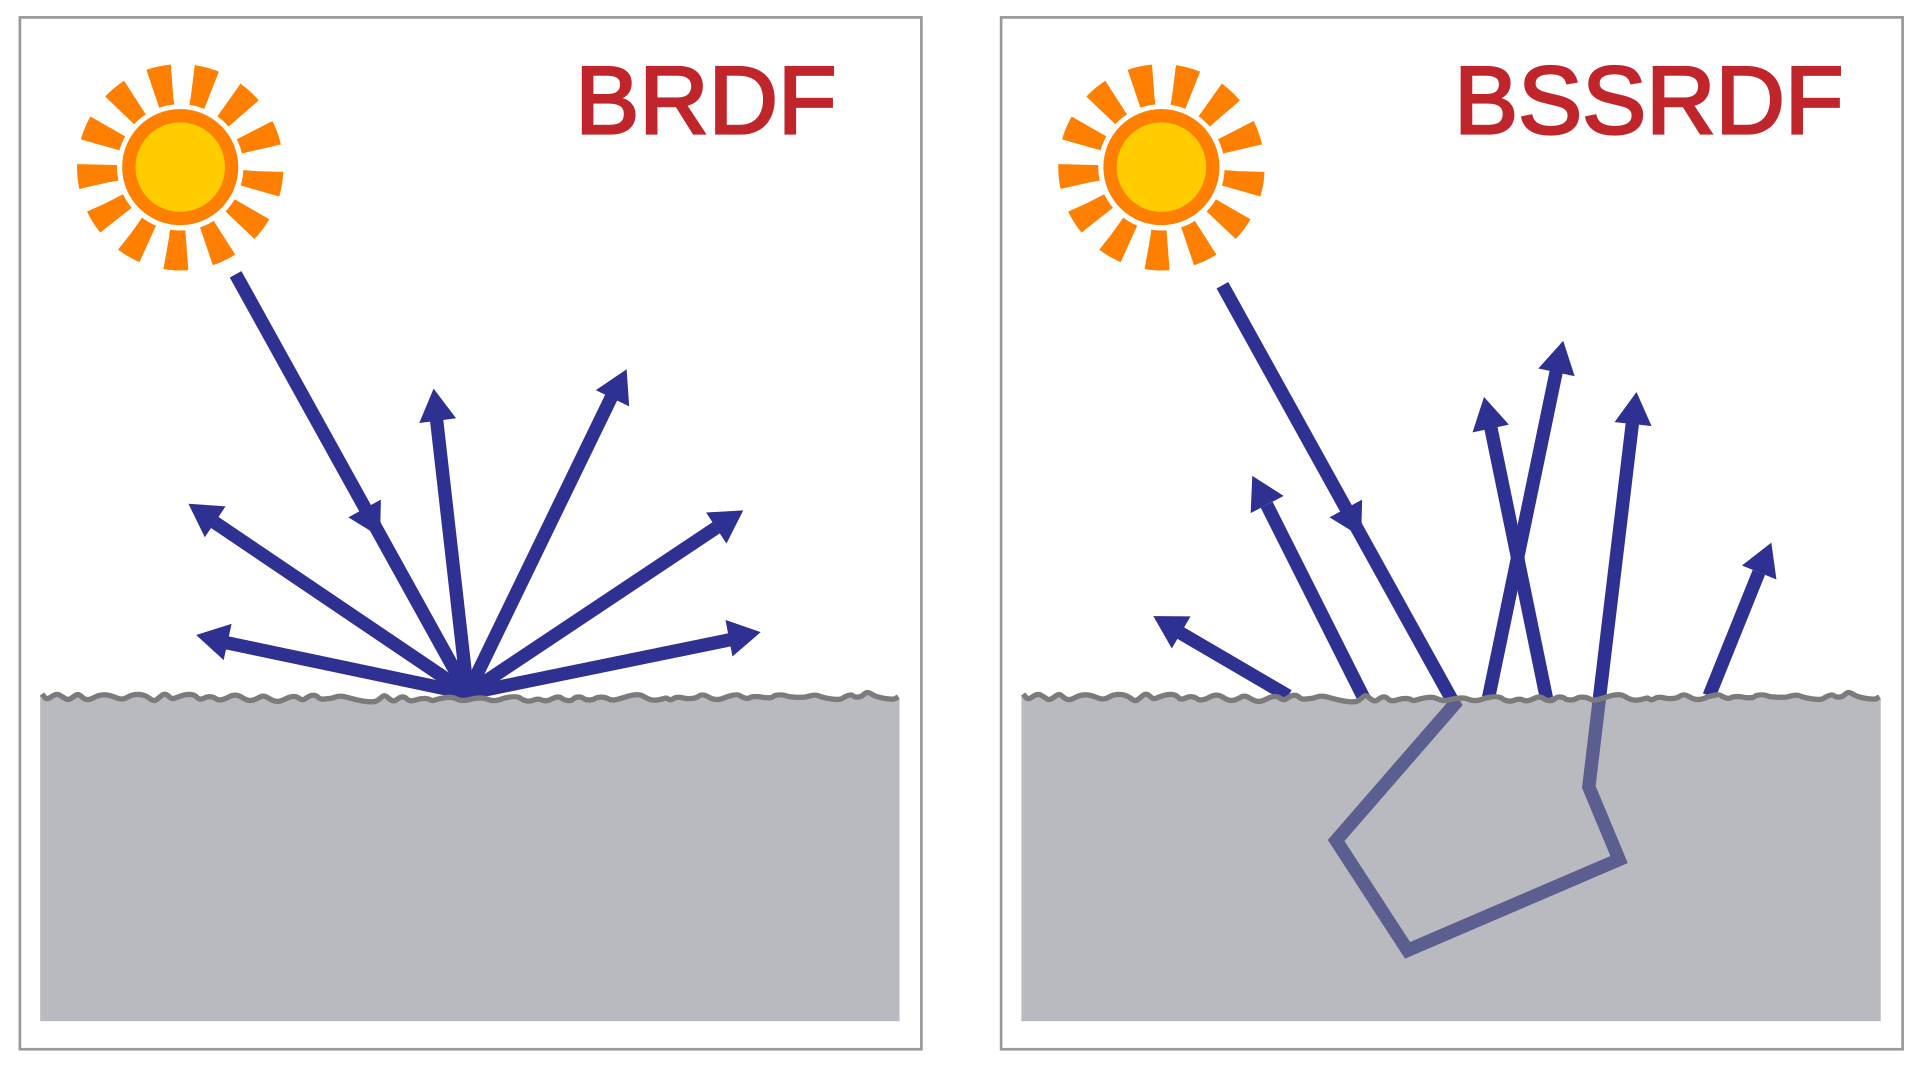
\includegraphics[width=0.5\textwidth]{pics/bssrdf.png}
	\caption{Ilustrație a fenomenului de subsurface scattering. Razele intră în obiect și ies în alt punct\protect\footref{fn:wiki}}
	\label{fig:sss}
\end{figure}

Pentru a fi considerat pentru uz PBR (physically based rendering), un BRDF
este supus unor constrângeri care s-au standardizat în literatura de specialitate
(Lafortune et. al. 1994~\cite{Lafortune}):

\begin{enumerate}
	\item \textbf{Pozitivitatea}: $f_r(\mathbf{x}, \omega_i, \omega_o) \geq 0$, pentru orice $\mathbf{x}$, $\omega_i$ și $\omega_o$.
	\item \textbf{Conservarea energiei}: $\int_{\Omega_+} f_r(\mathbf{x}, \omega_i, \omega_o) (\omega_i \cdot \mathbf{n}) \diff \omega_i \leq 1$, pentru orice $\mathbf{x}$ și $\omega_o$.
	\item \textbf{Reciprocitatea Helmholtz}: $f_r(\mathbf{x}, \omega_i, \omega_o) = f_r(\mathbf{x}, \omega_o, \omega_i)$, pentru orice $\mathbf{x}$, $\omega_i$ și $\omega_o$.
\end{enumerate}

Dacă modelul nu respectă cel puțin aceste constrângeri, algoritmul de Path Tracing
poate să nu conveargă sau să producă rezultate nerealiste.

Există multe modele de distribuție în literatura de specialitate, cu grade diferite de complexitate și
reprezentare a fenomenelor fizice. Printre primele modele apărute se numără
modelul Lambertian (bazat pe modelul perfect difuz descris de Lambert în 1760~\cite{Lambert}),
modelul Phong (1975)~\cite{Phong} împreună cu optimizarea Blinn-Phong (1977)~\cite{BlinnPhong},
precum și modele speculare bazate pe microfațete (\cite{TorranceOld}, \cite{CookTorrance}).
Vom prezenta în continuare funcțiile de distribuție pentru aceste modele, fără a intra
în prea multe detalii matematice de derivare. Pentru acestea, cititorul este îndrumat
spre literatura de specialitate.

\subsubsection*{Modelul Lambertian}

Modelul Lambertian modelează reflectanța difuză a unui material. Dându-se o normală
la suprafață $\mathbf{n}$ și o direcție de incidență $\omega_i$, reflectanța Lambertiană
se calculează ca produsul dintre albedo-ul materialului, normala și direcția de incidență:
$L = \rho \cdot (\omega_i \cdot \mathbf{n})$. Acest model trebuie totuși normalizat pentru
a fi transformat într-un BRDF - o derivare folosind concepte de bază se găsește în~\cite{LambertBRDF}.
BRDF-ul rezultat este:
\begin{equation}\label{eq:lambert}
	f_{Lambert}(\mathbf{x}, \omega_i, \omega_o) = \frac{\rho}{\pi},
\end{equation}
unde $\rho$ este culoarea materialului (albedo). Observăm că termenul de $\cos$ cu
nu apare aici. Acesta este inclus implicit în ecuația de randare~\ref{eq:light_transport}.

Definiția exactă pentru albedo
seamănă destul de mult cu termenul integral din ecuația de transport a luminii:
\begin{equation}
	\rho = \int_{\Omega_+} f_r(\mathbf{x}, \omega_i, \omega_o) (\omega_i \cdot \mathbf{n}) \diff \omega_i,
\end{equation}
deoarece măsoară reflectanța unei suprafețe perfect difuze când este iluminată
uniform de la toate direcțiile de lumină cu radianță unitară.

\subsubsection*{Modelul Phong}

În adiție față de modelul Lambertian, modelul Phong adaugă un termen de reflexie
speculară. Modelul inițial introdus de Phong în 1975~\cite{Phong} nu este un BRDF
propriu-zis (nu respectă constrângerile definite anterior), ci mai degrabă un model de iluminare. O adaptare a acestuia pentru
a fi folosit ca BRDF a fost făcută de Lafortune și Willems în 1994~\cite{Lafortune}.

Definiția BRDF-ului din publicație este:
\begin{equation}\label{eq:phong}
	f_{Phong}(\mathbf{x}, \omega_i, \omega_o) = k_d\frac{1}{\pi} + k_s\frac{n + 2}{2\pi}(\omega_r \cdot \omega_o)^n,
\end{equation}
unde $k_d$ și $k_s$ sunt coeficienții de reflexie difuză și speculară, definiți
în intervalul $[0, 1]$, $n$ este exponentul de reflexie speculară iar $\omega_r$ este
direcția de reflexie perfect speculară a luminii. De remarcat că termenul de $\cos$
este restricționat să nu fie mai mic decât zero. Un exponent $n$ mare va duce la o
reflexie mai concentrată, în timp ce unul mic va duce la o reflexie mai difuză.
Ideal, pentru a nu viola legea conservării a energiei, trebuie să nu reflectăm mai multă lumină
decât am primit. Acest lucru se poate obține prin condiția $k_d + k_s \leq 1$.

\subsubsection*{Modelul Microfațetelor}
Introdusă în anul 1982 de Cook și Torrance~\cite{CookTorrance}, teoria microfațetelor postulează ideea că
majoritatea materialelor de diferite grade de luciu sunt compuse din microfațete
(drepte sau modelate de curbe simple - vezi Figura~\ref{fig:microfacet}). Acestea sunt orientate aleator și
sunt descrise de două lucruri: distribuția orientării lor și profilul (i.e.,
cum sunt dispuse pe suprafață). Două suprafețe diferite pot avea aceeași distribuție
dar profiluri diferite, ceea ce duce la aspecte diferite ale materialului (vezi Figura~\ref{fig:microfacet_profiles}).

Asumpția de bază a modelului funcționează prin agregarea comportamentului
luminii de la nivel microscopic (microfațete) la nivel macroscopic (suprafața modelată).
Este același principiu pe care funcționează și monitoarele - fiecare pixel este compus
din subpixeli care emit lumină de diferite culori (RGB), dar la distanța la care
ne aflăm noi de monitor nu mai putem distinge acești subpixeli individuali, ci doar
culoarea agregată a pixelului.

Un aspect foarte important care trebuie luat în considerare este profilul microfațetelor.
Acestea pot fi reprezentate fizic de câmpuri de înălțimi, iar zonele dintre două
vârfuri adiacente pot fi obstrucționate și private de lumină. Acest fenomen este
mai departe categorizat în două:

\begin{itemize}
	\item \textbf{Mascare (Masking)}: microfațeta este obstrucționată din perspectiva observatorului
	\item \textbf{Umbrire (Shadowing)}: microfațeta este obstrucționată din perspectiva sursei de lumină.
\end{itemize}

De asemenea, un alt fenomen extrem ce trebuie luat în considerare este cel al
retroreflexiei. Acesta este manifestat drept o reflexie a luminii înapoit pe direcția
incidentă (spre deosebire de o reflexie speculară), preponderent mai ales la unghiuri
de incidență mari. Totuși, există materiale care prezintă acest fenomen mai pronunțat,
precum cele reflectorizante sau textile.
În acest model teoretic, retroreflexia apare
atunci când lumina este reflectată de mai multe ori între microfațete. O ilustrație
intuitivă a tuturor acestor fenomene importante se poate vedea în Figura~\ref{fig:microfacet_effects}.

\begin{figure}[ht]
	\centering
	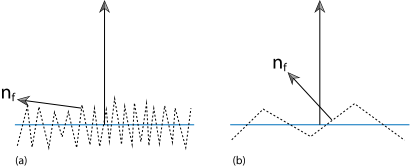
\includegraphics[width=0.7\textwidth]{pics/microfacet.png}
	\caption{Profilul microfațetelor pentru materiale dure (stânga), respectiv lucioase (dreapta)\protect\footref{pbr-book}}
	\label{fig:microfacet}
\end{figure}

\begin{figure}[ht]
	\centering
	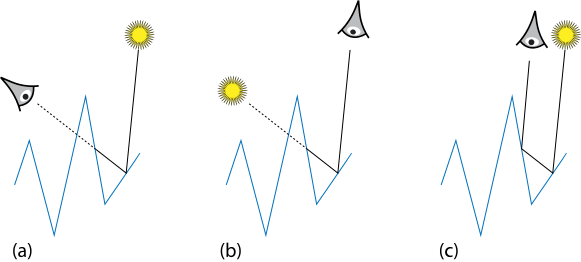
\includegraphics[width=0.7\textwidth]{pics/microfacet_effects.png}
	\caption{Efecte geometrice ale microfațetelor: mascare (a), umbrire (b) și retroreflexie (c)\protect\footref{pbr-book}}
	\label{fig:microfacet_effects}
\end{figure}

\begin{figure}[ht]
	\centering
	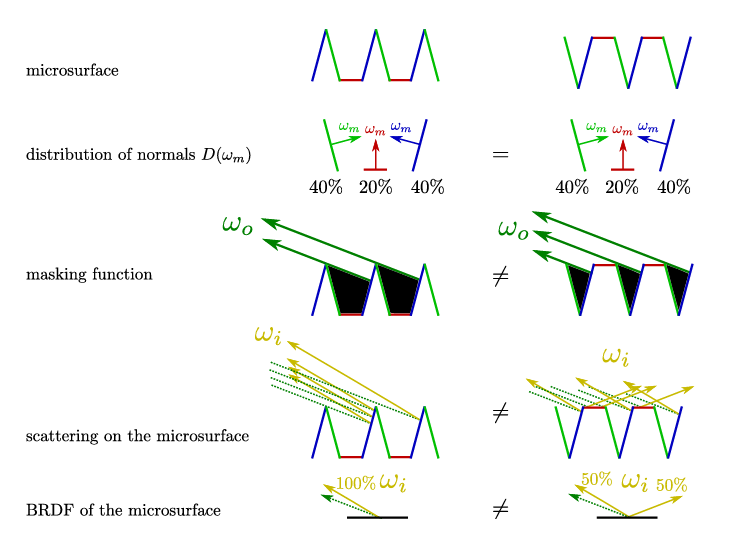
\includegraphics[width=0.7\textwidth]{pics/masking.png}
	\caption{Diferite profiluri de microfațete pentru aceeași distribuție. \copyright Heinz~\cite{HeitzMasking}}
	\label{fig:microfacet_profiles}
\end{figure}

O să concluzionăm prin a prezenta unul dintre primele și cele mai cunoscute BRDF-uri
bazate pe teoria microfațetelor - descris de Torrance și Sparrow în 1967~\cite{TorranceOld}.
În continuare, vom nota cu $\omega_i$ direcția de incidență, cu $\omega_o$ direcția de ieșire,
și cu $\omega_h$ normala microfațetei. Notăm funcția de distribuție a normalelor ca
$D(\omega_h)$. De notat că această funcție este normalizată, adică
\begin{equation}\label{eq:d_norm}
	\int_{\Omega} D(\omega_h)\cos \theta_h \diff \omega_h = 1.
\end{equation}
Ecuația~\ref{eq:d_norm} este o condiție necesară pentru plauzibilitatea modelului, iar
intuitiv reprezintă faptul că orice rază incidentă la suprafață de-a lungul macronormalei $n$ va
intersecta microfațetele o singură dată.

Pentru a ține cont de efectele de mascare și umbrire, ne trebuie o altă
funcție de distribuție care să determine ce porțiune din microfațete sunt vizibile
în funcție de direcția de incidență (mascare) și de direcția de ieșire (umbrire).
Această distribuție poate fi modelată separat (pentru o singură direcție) de
către funcția $G_1(\omega, \omega_h)$ a lui Smith, introdusă în 1967~\cite{SmithG1}.
Aceasta modelează proporția microfațetelor cu normala $\omega_h$ care sunt vizibile
din direcția $\omega$.
O formă generală a acestei funcții este:
\begin{equation}\label{eq:g1}
	G_1(\omega, \omega_h) = \frac{1}{1 + \Lambda(\omega, \omega_h)},
\end{equation}
unde $\Lambda(\omega)$ este o funcție nespecificată. Totuși, ea trebuie aleasă
pentru a satisface o constrângere de vizibilitate. Concret, aria $\diff A$ a suprafeței
văzută sub un unghi $\theta$ format între normala la suprafață $n$ și direcția de observare
$\omega$ trebuie să fie egală cu aria microfațetelor vizibile din aceeași direcție (vezi Figura~\ref{fig:microfacet_visible}):
\begin{equation}\label{eq:ndf}
	\cos\theta = \int_{\Omega} G_1(\omega, \omega_h) \max(0, \cos \theta) D(\omega_h) \diff \omega_h,
\end{equation}
unde adăugarea factorului $\max(0, \cos \theta)$ ne asigură că nu luăm în considerare microfațetele
care sunt orientate în direcția opusă observatorului.

\begin{figure}[ht]
	\centering
	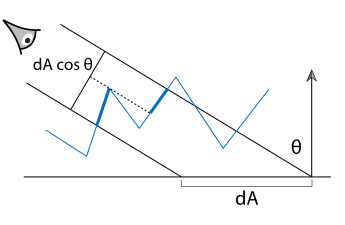
\includegraphics[width=0.5\textwidth]{pics/microfacet_visible.png}
	\caption{Ilustrație a vizibilității microfațetelor sub un unghi $\theta$\protect\footref{pbr-book}}
	\label{fig:microfacet_visible}
\end{figure}

Pentru un model corect trebuie să ținem cont și de mascare și de umbrire simultan.
Cu alte cuvinte, trebuie să calculăm proporția microfațetelor vizibile din ambele direcții.
Astfel, avem nevoie de o funcție $G_2(\omega_i, \omega_o, \omega_h)$ care să depindă
de toate cele trei direcții. O tehnică comună (Walter et. al.~\cite{WalterSmithG2}) este să se aproximeze această funcție
prin produsul a doi termeni separabili Smith $G_1$:
\begin{equation}
	G_2(\omega_i, \omega_o, \omega_h) = G_1(\omega_i, \omega_h)G_1(\omega_o, \omega_h).
\end{equation}
Deși nu este o soluție perfectă, căci nu ține cont de corelațiile dintre microfațete,
această aproximare este suficient de bună pentru a fi folosită în practică.

În final, modelul Torrance-Sparrow are și o componentă speculară modelată de legea
lui Fresnel. Presupunerea modelului este că microfațetele sunt perfect reflectante
și că reflexia speculară este dată de reflexia totală a luminii pe suprafață.
BRDF-ul Torrance-Sparrow este definit ca:
\begin{equation}
	f_{TS}(\mathbf{x}, \omega_i, \omega_o) = \frac{D(\omega_h)G_2(\omega_i, \omega_o, \omega_h)F(\omega_o)}{4(\omega_i \cdot \mathbf{n})(\omega_o \cdot \mathbf{n})},
\end{equation}
care poate fi simplificată sub asumpția că vizibilitatea microfațetelor este independentă
de orientarea acestora:
\begin{equation}\label{eq:ts}
	f_{TS}(\mathbf{x}, \omega_i, \omega_o) = \frac{D(\omega_h)G_2(\omega_i, \omega_o)F(\omega_o)}{4(\omega_i \cdot \mathbf{n})(\omega_o \cdot \mathbf{n})}.
\end{equation}

Frumusețea acestui model generalizat este faptul că acceptă diferite distribuții
de microfațete și funcții Fresnel, deci poate fi folosit atât pentru metale cât
și pentru materiale dielectrice. În plus, modelul este destul de simplu pentru a
putea fi folosit în practică, dar suficient de complex pentru a modela fenomene
fizice complexe.

\subsection{Strategii de eșantionare a direcțiilor de ieșire}

Ce am prezentat mai devreme despre funcțiile de distribuție a reflectanței
sunt expresiile acestora și modul în care se evaluează. Concret, evaluarea
BRDF-ului presupune cunoștința în prealabil a direcției de incidență și a celei
de ieșire. Într-un algoritm de Path Tracing, la fiecare pas al recursivității
se cunoaște doar direcția incidentă (începând cu prima rază pornită de la observator),
urmând să se determine, după intersecția cu o suprafață, direcția de ieșire (care
va constitui direcția incidentă pentru următoarea rază ș.a.m.d.). Această
direcție de ieșire poate fi aleasă aleator sau conform unei strategii de eșantionare.
În orice caz, fiind un algoritm Monte Carlo, se va ține cont de distribuția strategiei
de eșantionare și se va pondera rezultatul contribuției reflectanței în consecință.

Așa cum am discutat în
secțiunea~\ref{sec:is}, eșantionarea bazată pe importanță este crucială pentru
a obține o convergență rapidă a algoritmului. Dacă BRDF-ul unui material modelează
o suprafață speculară (poate chiar o oglindă perfectă), atunci distribuția
direcțiilor de ieșire va fi foarte îngustă, apropiindu-se de funcția delta Dirac:
\begin{equation}
	\begin{aligned}
		 & \delta(x) = \begin{cases}
			               \infty, & x = 0,    \\
			               0,      & x \neq 0.
		               \end{cases},                \\
		 & \int_{-\infty}^{\infty} \delta(x) \diff x = 1.
	\end{aligned}
\end{equation}
Folosind o eșantionare uniformă (\ref{eq:uniform_sampling}), această distribuție va fi eșantionată neoptim,
iar marea majoritate a direcțiilor generate nu vor contribui la radianța observată,
având probabilitate 0 (nefiind pe direcția de reflexie).

Pentru eșantionare, ne trebuie un generator de numere aleatoare. Fie $\xi_1$ și $\xi_2$
numere aleatoare din intervalul $[0, 1]$ (alese conform unei distribuții uniforme).
Aceste numere vor fi folosite în strategiile descrise jos pentru a genera direcții
de ieșire. De asemenea, facem precizarea că metodele prezentate mai jos presupun
că ne aflăm în sistemul de coordonate tangent la suprafață $(\mathbf{t}, \mathbf{n}, \mathbf{b})$, cu normala $\mathbf{n}$
orientată în sus, $\mathbf{n} = (0, 1, 0)$. Câteva metode presupun coordonatele sferice $(\theta, \phi)$,
din care putem transforma în cele carteziene folosind formulele:
\begin{equation}
	\begin{aligned}
		\mathbf{x} & = \sin \theta \cos \phi, \\
		\mathbf{y} & = \cos \theta,           \\
		\mathbf{z} & = \sin \theta \sin \phi.
	\end{aligned}
\end{equation}

Cea mai simplă strategie este eșantionarea emisferică uniformă. Aceasta presupune
alegerea aleatoare a unei direcții de ieșire din emisfera superioară a punctului
de intersecție. Considerând coordonatele sferice $(\theta, \phi)$, formulele
de transformare, împreună cu probabilitatea eșantionului, sunt:
\begin{equation}\label{eq:uniform_sampling}
	\begin{aligned}
		\theta & = \arccos \xi_1,  \\
		\phi   & = 2\pi \xi_2,     \\
		pdf    & = \frac{1}{2\pi}.
	\end{aligned}
\end{equation}

Această strategie este foarte brută. Nu ține cont de distribuția BRDF-ului și
poate să genereze multe direcții care nu contribuie la radianța observată (mai ales
în cazul unui material specular - atunci rezultatele ar fi chiar greșite). O variantă mai bună (dar care tot nu ține cont de material) este eșantionarea ponderată
de cosinusul unghiului de ieșire. Această strategie ponderează probabilitatea
eșantionului cu $\cos \theta$ (unghiul făcut cu normala) și are la bază principiul
cosinusului Lambertian. Formulele sunt:
\begin{equation}\label{eq:cosine_sampling}
	\begin{aligned}
		\theta & = \arccos \sqrt{\xi_1},    \\
		\phi   & = 2\pi \xi_2,              \\
		pdf    & = \frac{\cos \theta}{\pi}.
	\end{aligned}
\end{equation}

Derivări ale ecuațiilor~\ref{eq:uniform_sampling} și~\ref{eq:cosine_sampling} se pot găsi
în~\cite{sampling}.

Am discutat în secțiunea~\ref{sec:is} despre eșantionarea bazată pe importanță.
În contextul de față, aceasta înseamnă alegerea unei direcții de ieșire care să
contribuie cât mai mult la radianța observată. Acest lucru este realizat prin
modelarea unei distribuții de eșantionare care să aproximeze cât mai bine distribuția
BRDF-ului.

În cazul unui material Lambertian, definit de ecuația~\ref{eq:lambert}, observăm
că distribuția BRDF-ului este constantă are aceeași formă uniformă ca eșantionarea
uniformă. Astfel, am fi tentați să concluzionăm că putem folosi
ecuațiile~\ref{eq:uniform_sampling} pentru a genera direcții de ieșire. Totuși,
am omite factorul de $\cos$ care apare în ecuația de randare~\ref{eq:light_transport}.
Așadar, distribuția este mai degrabă una ponderată de cosinus, și e mult mai bine
să folosim ecuațiile~\ref{eq:cosine_sampling}. De fapt, eșantionarea uniformă este
inutilă în aproape toate cazurile, iar rezultatele ei dezamăgitoare se pot
observa în Figura~\ref{fig:eval-uniform}.

În cazul unui material Phong definit de BRDF-ul~\ref{eq:phong}, o distribuție
bună este greu de calculat. Autorii remarcă faptul că partea speculară nu poate
fi integrată analitic și că eșantionarea acesteia se face printr-un proces
Monte Carlo. Voi omite detaliile matematice aici, pentru că nu prezintă interes;
cititorul este îndrumat spre~\cite{Lafortune} pentru detalii.

Eșantionarea modelului Torrance-Sparrow este intuitivă. Deoarece factorul
predominant este distribuția micronormalelor $D(\omega_h)$, eșantionarea
se poate face fix pe această distribuție. În acest caz, se va reflecta
raza de incidență $\omega_i$ în jurul normalei eșantionate pentru a obține
direcția de ieșire $\omega_o$. Totuși, o metodă mult mai eficientă pentru
unghiuri de incidență mari o reprezintă eșantionarea normalelor vizibile.
Reamintim că ecuația~\ref{eq:ndf} trebuie să fie satisfăcută pentru a obține
o distribuție corectă. Această ecuație descria proporția microfațetelor vizibile
sub un unghi $\theta$ față de normala la suprafață. Putem rearanja ecuația
pentru a obține distribuția micronormalelor într-o direcție $\omega$:
\begin{equation}
	D_{\omega}(\omega_h) = \frac{G_1(\omega, \omega_h)\max(0, \cos \theta)D(\omega_h)}{\cos \theta_h}.
\end{equation}
Un ultim aspect de luat în considerare în calculul probabilității de eșantionare
este faptul că această distribuție reprezintă normalele în jurul micronormalei $\omega_h$,
în timp ce BRDF-ul ține cont de direcția de incidență $\omega_i$. Astfel, trebuie făcută
o ajustare de schimbare de variabilă. Procesul este detaliat în~\cite{PbrBookNdf}.
Densitatea de probabilitate se modifică astfel cu un factor de $\dfrac{1}{4(\omega_o \cdot \omega_h)}$.

\subsection{Next Event Estimation}

Next Event Estimation (NEE) este o strategie de eșantionare bazată pe importanță
multiplă (MIS) care presupune o combinație între eșantionarea BRDF-ului și a
surselor de lumină. Aceasta reprezintă o îmbunătățire masivă a convergenței
algoritmului de Path Tracing, deoarece multe dintre direcțiile generate de
eșantionarea BRDF-ului în sine pot să nu ajungă să intersecteze o sursă de lumină
și, implicit, nu vor contribui la radianța observată. În schimb, eșantionarea
surselor de lumină la fiecare pas al recursivității ajută mult în acest sens.
Astfel, eșantionarea luminii calculează iluminarea directă, în timp ce eșantionarea
BRDF-ului calculează iluminarea indirectă. În final, aceste două contribuții
sunt combinate probabilistic pentru a obține rezultatul final. Avantajele acestei
metode se pot observa în Figura~\ref{fig:nee}.

\begin{figure}[ht]
	\centering
	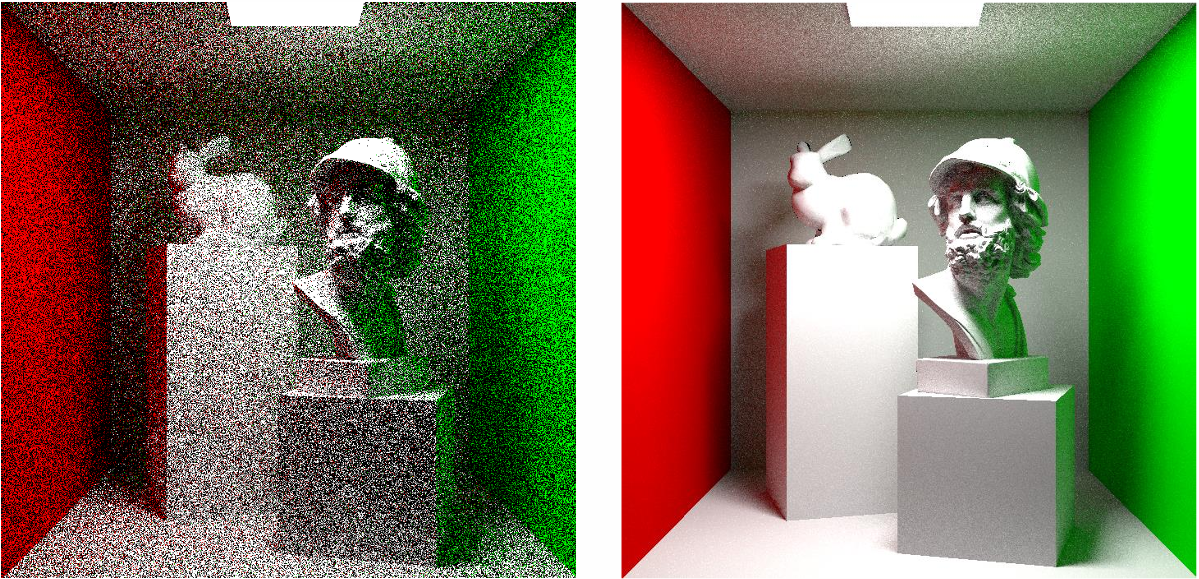
\includegraphics[width=\textwidth]{pics/nee.png}
	\caption{Comparație între eșantionare a BRDF-ului (stânga) și NEE (dreapta)\protect\footnotemark}
	\label{fig:nee}
\end{figure}
\footnotetext{\copyright\url{https://www.cg.tuwien.ac.at/sites/default/files/course/4411/attachments/08_next\%20event\%20estimation.pdf}. Accesat 24.06.2024.}

Ideea de bază este de a combina cele două contribuții (directă și indirectă)
cu o pondere în $[0, 1]$. Aceasta poate fi ori constantă (e.g., 0 sau 1) ori
bazată pe o euristică (precum cele studiate de Veach - balance sau power~\cite{Veach,VeachPower}).
Formula generală pentru a combina cele două contribuții este:
\begin{equation}\label{eq:nee}
	L(\mathbf{x}, \omega_i, \omega_o) = w\cdot f_{r}(\mathbf{x}, \omega_i, \omega_o) L_e(\mathbf{x}, \omega_i, \omega_o),
\end{equation}
unde $w$ este factorul de ponderare, $f_{r}$ este BRDF-ul materialului și $L_e$
este radianța emisă de sursa de lumină (normalizată cu probabilitatea de eșantionare).
\section{Accelerare Hardware}

Până acum am discutat despre aspectele teoretice ale domeniului. În practică,
algoritmii de tip Monte Carlo precum Path Tracing sunt foarte costisitori din
punct de vedere computațional. Prin natura lor, aceștia sunt algoritmi paraleli
și pot beneficia de accelerare hardware precum GPU-urile, care sunt fundamental
concepute în jurul unei arhitecturi SIMD. În mod tradițional, totuși, algoritmii
offline folosiți în motoarele grafice de producție (Blender Cycles\footnote{\url{https://www.cycles-renderer.org/}. Accesat 24.06.2024.},
Autodesk Arnold\footnote{\url{https://www.autodesk.co.uk/products/arnold/overview?term=1-YEAR&tab=subscription}. Accesat 24.06.2024.},
Chaos V-Ray\footnote{\url{https://www.chaos.com/3d-rendering-software}. Accesat 24.06.2024.})
sunt rulați pe CPU-uri, în parte deoarece este
mult mai facil de dezvoltat și extins un program care rulează pe CPU. De pildă,
un framework multi-vendor, OpenCL\footnote{\url{https://www.khronos.org/api/opencl}. Accesat 24.06.2024.},
nu a primit prea mult suport în motoarele grafice de producție precum Cycles sau Arnold
(dar tool-uri noi precum HIP\footnote{\url{https://github.com/ROCm/HIP}. Accesat 24.06.2024.}
încep să primească suport\footnote{\url{https://code.blender.org/2021/11/next-level-support-for-amd-gpus/}. Accesat 24.06.2024.}).
Povestea este puțin mai
fericită în tabăra verde (Nvidia), care are suport mai răspândit pentru framework-ul
CUDA. Totuși, într-un context de randare în timp real, CUDA este o opțiune ce
aduce un overhead sesizabil.

În industria real-time (specific jocurilor video), accelerarea hardware este
esențială. Totodată, se preferă să se folosească un API cât mai aproape de driver
și cu o amprentă cât mai mică asupra sistemului. De aceea, se folosesc API-uri
precum Vulkan sau DirectX 12 în defavoarea CUDA sau OpenCL. Acestea din urmă sunt
mai degrabă folosite în aplicații de tip offline, unde timpul de randare nu este
atât de critic.

\subsection{Vulkan}

Vulkan a fost dezvoltat cu scopul de a fi un succesor al OpenGL și de a utiliza
eficient hardware-ul modern, oferind uneltele de optimizare necesare
pentru a distribui sarcini pe mai multe fire de execuție\footnote{\url{https://www.vulkan.org/}. Accesat 24.06.2024.}.
A fost adoptat la scară largă în industria jocurilor video\footnote{\url{https://www.pcgamingwiki.com/wiki/List_of_Vulkan_games}. Accesat 24.06.2024.}
și continuă să se dezvolte spre a fi un standard în industrie.
De remarcat că acest API oferă suport pentru Ray Tracing accelerat hardware\footnote{\url{https://docs.vulkan.org/guide/latest/extensions/ray_tracing.html}. Accesat 24.06.2024.}.

\subsection{DirectX 12}

DirectX 12 este cel mai popular API modern de grafică în industria jocurilor video\footnote{\url{https://www.pcgamingwiki.com/wiki/List_of_Direct3D_12_games}. Accesat 24.06.2024.}.
dezvoltat de Microsoft pentru a fi folosit pe platformele Windows și Xbox\footnote{\url{https://learn.microsoft.com/en-us/windows/win32/direct3d12/what-is-directx-12-}. Accesat 24.06.2024.}.
Acesta oferă avantaje similare cu cele oferite de Vulkan, însă și acesta este
un API de nivel scăzut, notoriu pentru dificultatea de a fi folosit la potențialul său maxim.
Acesta oferă suport pentru Ray Tracing accelerat hardware
prin intermediul extensiei DirectX Raytracing (DXR).\footnote{\url{https://devblogs.microsoft.com/directx/announcing-microsoft-directx-raytracing/}. Accesat 24.06.2024.}.
Acesta a devenit standardul în industrie pentru randarea în timp real și este
adoptat în majoritatea noilor lansări AAA de pe piață\footnote{\url{https://www.pcgamingwiki.com/wiki/List_of_games_that_support_ray_tracing}. Accesat 24.06.2024.}.
Acest API, împreună cu extensia DXR, este folosit în acest proiect pentru
a accelera randarea Path Tracing pe GPU (vezi capitolul~\ref{sec:implementare}).

\chapter{\label{sec:solutie}Soluția Propusă}

Proiectul de față dezvoltă un motor de randare bazat pe Ray Tracing Whitted și Path Tracing, cu suport
pentru accelerare hardware folosind API-ul DirectX 12. Acesta este scris în C++20,
iar algoritmii de Ray Tracing sunt implementați în cadrul HLSL. Proiectul a fost
dezvoltat pornind de un exemplu oferit public de Microsoft~\cite{Schelet},
care oferă un schelet bun de DirectX 12 și este un punct de plecare ce oferă
majoritatea boilerplate-ului necesar pentru a începe dezvoltarea. A fost modificat acest cod
suport pentru a extinde funcționalitatea cu încă un set de shadere pentru Path Tracing și
a suporta noi tipuri de suprafețe (e.g., unghi solid - Figura~\ref{fig:solid-angle}). De asemenea,
acesta a fost extins cu multe alte funcționalități, pe care le vom detalia în acest
capitol.

\begin{figure}[!htb]
	\centering
	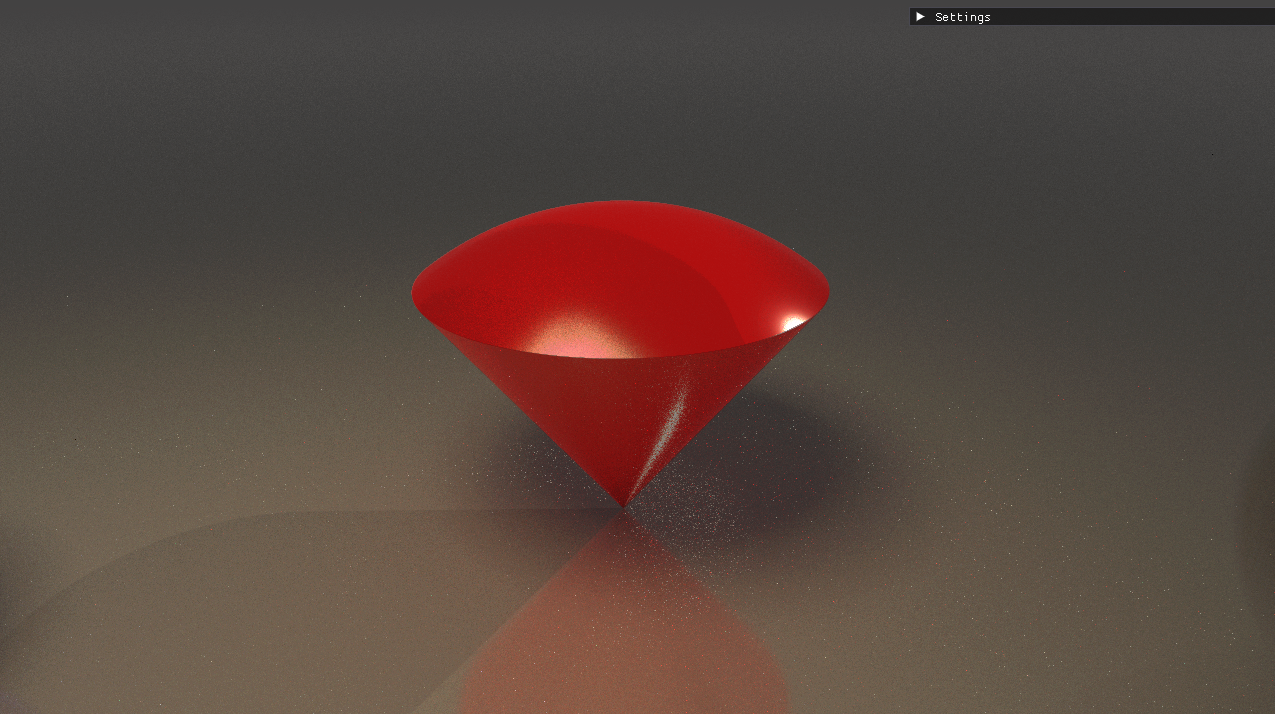
\includegraphics[width=\textwidth]{pics/solid-angle.png}
	\caption{Unghi solid reprezentat drept câmp de distanță\protect\footnotemark}
	\label{fig:solid-angle}
\end{figure}
\footnotetext{Formula câmpului a fost preluată de la adresa~\url{https://www.shadertoy.com/view/Xds3zN}. Accesat 24.06.2024.}

Pe scurt, am implementat, pe lângă codul din schelet:
\begin{itemize}
	\item Un meniu de setări pentru a controla parametrii de randare și a manipula scena
	\item Suport pentru reîncărcarea aplicației în timp real (la comandă sau automat la modificarea unor setări de bază)
	\item Un sistem de mișcare și rotire a camerei, folosind mouse-ul și tastele WASD
	\item Un sistem de materiale physically based, bazat pe modelul Disney principled BSDF~\cite{Disney,DisneyBSDF}.
	\item Un algoritm de Path Tracing care folosește acest sistem de materiale. Particularități:
	      \begin{itemize}
		      \item Algoritmul este accelerat hardware folosind API-ul DXR
		      \item Suport pentru reflexii, refracții, umbre, iluminare globală și multiple surse de lumină
		      \item Suport pentru configurarea parametrilor (a se vedea Figura~\ref{fig:imgui-renderer})
		      \item Suport pentru eșantionare bazată pe importanță multiplă și Next Event Estimation
		      \item Metodă de ruletă rusească pentru terminarea prematură (unbiased) a recursivității
		      \item Suport pentru acumulare progresivă.
	      \end{itemize}
\end{itemize}

\section{Tehnici de accelerare a convergenței}\label{sec:options}
Algoritmul de bază prezentat în pseudocodul~\ref{alg:path_tracing} a fost
augmentat cu mai multe tehnici de accelerare a convergenței, majoritatea fiind
descrise în secțiunea~\ref{sec:path_tracing}. Multe dintre acestea sunt configurabile
din meniu, iar unele sunt activate implicit.
\begin{itemize}
	\item \textbf{Next Event Estimation} - la fiecare pas se selectează o lumină (sau toate)
	      din scenă și se eșantionează cu importanță multiplă contribuția directă și indirectă.
	      În formula~\ref{eq:nee} s-a folosit pentru calculul ponderii $w$ euristica puterii 2:
	      \begin{equation}
		      w = \dfrac{pdf_L^2}{pdf_f^2 + pdf_L^2}.
	      \end{equation}
	      Această optimizare se efectuează implicit și nu este configurabilă.
	\item \textbf{Eșantionare a unei singure lumini} - pentru ca algoritmul să nu piardă
	      performanță dramatic în cazul în care există multe surse de lumină, se poate alege
	      aleator o singură sursă de lumină la fiecare pas pe care să se aplice NEE. Rezultatul
	      final este ponderat apoi cu probabilitatea de eșantionare a sursei de lumină (în acest
	      caz, $1/N$, unde $N$ este numărul de surse de lumină). Această optimizare poate
	      fi dezactivată din meniu (este activată implicit).
	\item \textbf{Eșantionare bazată pe importanță} - alegerea unei noi direcții de ieșire
	      pentru pasul recursiv se face folosind o eșantionare concepută pentru a aproxima
	      distribuția de probabilitate a normalelor microfațetelor (vezi secțiunile~\ref{sec:is}, \ref{sec:pbr} și \ref{sec:disney}).
	      Această optimizare este activată implicit și poate fi schimbată cu alte două
	      tehnici de eșantionare: uniformă sferică, respectiv ponderată de cosinusul unghiului
	      de ieșire.
	\item \textbf{Ruleta rusească} - o tehnică unbiased care termină prematur
	      recursivitatea pentru a evita pierderea de timp în cazul în care contribuția pe o cale
	      este foarte mică. Probabilitatea de eliminare este invers proporțională cu
	      contribuția acumulată până la acel pas. Pentru a nu introduce bias din cauza
	      energiei pierdute în terminarea prematură, contribuția acumulată se
	      ponderează la fiecare pas cu probabilitatea de terminare.
	      Această optimizare este activată implicit și poate fi configurată
	      prin modificarea adâncimii de la care se aplică.
\end{itemize}

\section{Suport pentru suprafețe implicite și analitice}
Motorul grafic suportă, pe lângă suprafețele tradiționale definite prin primitive
geometrice (e.g., triunghiuri), și suprafețe definite implicit (vezi secțiunea~\ref{sec:raymarching}) sau analitic.
Acestea se încadrează în AABB-uri care se folosesc în structura de accelerare BVH
oferită de DXR. Astfel, API-ul se ocupă de intersecția cu aceste încadrări, iar
mai departe se utilizează rutine specifice pentru a calcula intersecția precisă
cu suprafața definită. Pentru cele implicite, se folosesc funcții de distanță cu semn
și se aplică Ray Marching local (vezi secțiunea~\ref{sec:raymarching}). Pentru
suprafețele analitice, precum sferele și paralelipipedul, se folosesc formule
analitice pentru a calcula intersecția. Rutinele de intersecție pentru suprafețele
analitice sunt mult mai rapide decât cele de Ray Marching, dar nu oferă la fel
de multă flexibilitate creativă.

Ofer credite lui Inigo Quilez~\cite{iq} și Microsoft~\cite{Schelet} pentru formulele care definesc aceste
suprafețe.

\section{Sistemul de materiale}\label{sec:disney}

Sistemul de materiale este un BSDF compus ce combină mai mulți lobi definiți
de BRDF-uri și BTDF-uri. Modelul particular este denumit Disney Principled BSDF
și a fost introdus de Burley în 2012~\cite{Disney} ca un BRDF și extins în 2015~\cite{DisneyBSDF}
cu o serie de îmbunătățiri, precum un lob de transmisie. Acesta este modelul care
a fost folosit în producția cinematografică, începând cu filmul Wreck-It Ralph.

Modelul este principiat în sensul că deviază în mod subtil de la modelele fizice
pentru a oferi un control și o intuiție mai bună artistului. Astfel, acesta expune
o interfață simplă, cu parametri normalizați (în $[0, 1]$) care să se coreleze
cu proprietățile fizice ale materialelor, uneori alegând să nu aibe corespondență perfectă
cu realitatea ci mai degrabă un impact artistic. O ilustrație a parametrilor
disponibili în modelul din 2012 se poate vedea în Figura~\ref{fig:disney_params}.
\begin{figure}[!htb]
	\centering
	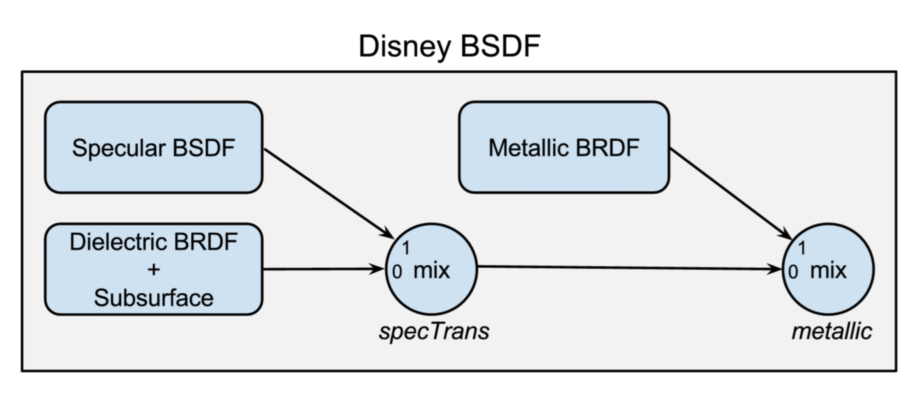
\includegraphics[width=\textwidth]{pics/disneybsdf.png}
	\caption{Compunerea BSDF-ului Disney Principled~\cite{DisneyBSDF}}
	\label{fig:disneybsdf}
\end{figure}

În lucrarea de față am ales să implementăm modelul din 2015, cu câteva modificări
care să ușureze dezvoltarea. Câteva implementări de referință sunt~\cite{DisneyHomework,DisneySchutte,GlslPathTracer}.
Menționăm faptul că distribuțiile prezentate în continuare vor folosi calcule
într-un sistem de coordonate local $(\mathbf{t}, \mathbf{b}, \mathbf{n})$,
pe când în implementare se folosește un sistem de coordonate local $(\mathbf{t}, \mathbf{n}, \mathbf{b})$,
unde $\mathbf{t}$ este tangenta, $\mathbf{n}$ este normala și $\mathbf{b}$ este bitangenta la suprafață.

\subsubsection*{Lobul difuz}
Reprezintă un model empiric ce încearcă să modeleze efectele
observate de Burley în setul de date MERL~\cite{MERL}: la unghiuri de incidență
mari, materialele lucioase au reflectanța scăzută, în timp ce materialele
dure au reflectanța crescută față de unghiul normal de incidență. Aceste
observații sunt prezise de reflexia Fresnel, motiv pentru care modelul propus
ține cont de aceasta:
\begin{equation}\label{eq:brdf_diffuse}
	f_d = \dfrac{albedo}{\pi}F_D(\omega_i, \omega_h)F_D(\omega_o, \omega_h),
\end{equation}
unde $F_D(\omega, \omega_h)$ este o modificare a aproximației lui Schlick~\cite{Schlick} a
reflexiei Fresnel pentru direcția de incidență $\omega$ și micronormala $\omega_h$
\begin{equation}
	\begin{aligned}\label{eq:f_d}
		F_D(\omega, \omega_h) & = 1 + (F_{D90} - 1)(1 - |\omega \cdot \omega_h|)^5,      \\
		F_{D90}               & = 0.5 + 2\cdot roughness\cdot |\omega_o \cdot \omega_h|.
	\end{aligned}
\end{equation}
Această modificare ignoră indicele de refracție al materialului și presupune
că nu există pierderi de energie incidentă la difuzie, ceea ce permite
BRDF-ului să depindă direct de o culoare $albedo$ specificată. De asemenea, termenul $F_{D90}$ este
ales astfel încât contribuția de tip retroreflexie să fie modulată, în funcție
de $roughness$, între 0.5 ($roughness = 1$) și 2.5 ($roughness = 0$). Această
modificare este strict empirică și, conform lui Burley, are un feedback pozitiv
din partea artiștilor.

Versiunea din 2015 transformă $f_d$ într-un BSDF cu componentă de dispersie
sub suprafață, care este simulată prin Path Tracing Volumetric (introdusă prima oară de Lafortune și Willems~\cite{Volumetric}),
dar acest algoritm este prea costisitor pentru randare în timp real.
Așadar, rămânem la BRDF-ul~\ref{eq:brdf_diffuse} și îl complementăm cu o aproximație
a acestui fenomen bazată pe legea Lommel-Seeliger\footnote{\url{https://phys.libretexts.org/Bookshelves/Astronomy__Cosmology/Planetary_Photometry_(Tatum_and_Fairbairn)/03\%3A_A_Brief_History_of_the_Lommel-Seeliger_Law}. Accesat 24.06.2024.}, așa cum este descris în~\cite{DisneyHomework}:
\begin{equation}
	f_{ss} = \dfrac{1.25\cdot albedo}{\pi} \left(F_{SS}(\omega_i, \omega_h)F_{SS}(\omega_o, \omega_h) \left(\dfrac{1}{|\omega_i \cdot \omega_h| + |\omega_o \cdot \omega_h|} - 0.5\right) + 0.5 \right),
\end{equation}
unde $F_{SS}$ este aceeași aproximare folosită pentru $F_D$ (\ref{eq:f_d}), dar cu o remapare $F_{SS90} = roughness\cdot (\omega_o\cdot \omega_h)^2$.

Într-un final, cele două componente sunt interpolate liniar de parametrul $subsurface$:
\begin{equation}\label{eq:disney_diffuse}
	f_{d} = (1 - subsurface)\cdot f_d + subsurface\cdot f_{ss}.
\end{equation}

\subsubsection*{Componenta de luciu (sheen)}

Materialele textile precum catifeaua sau mătasea au un luciu pronunțat la unghiuri
mari de incidență, cauzat de retroreflexie. Pentru a compensa pentru acest efect,
Burley a adăugat o componentă aditivă de luciu la BRDF-ul difuz (aceasta nu este
evaluată ca un lob separat). La fel cum a procedat și la difuz, Burley a folosit
un termen Fresnel modificat pentru a accentua retroreflexia:
\begin{equation}
	\begin{aligned}\label{eq:disney_sheen}
		f_{sheen} & = sheen\cdot C_{sheen}(1 - |\omega\cdot\omega_h|^5), \\
		C_{sheen} & = (1 - sheenTint) + sheenTint\cdot C_{tint},         \\
		C_{tint}  & = albedo/luminance(albedo),
	\end{aligned}
\end{equation}
unde $sheenTint$ este un parametru care controlează contribuția culorii materialului
la luciu. Reflexia speculară a unui dielectric este totuși acromatică, însă această
componentă modelează structura complexă a textilei și deci este lăsată la latitudinea
artistului cât de colorată să fie.

\subsubsection*{Lobul de reflexie speculară}

Reprezintă este un model BRDF de microfațete de tipul Torrance-Sparrow (vezi ecuația~\ref{eq:ts}):
\begin{equation}\label{eq:disney_specular}
	f_{sp} = \dfrac{D(\omega_h)G(\omega_i, \omega_o)F(\omega_o)}{4|\omega_i \cdot \mathbf{n} ||\omega_o \cdot \mathbf{n}|},
\end{equation}
Pentru distribuția microfațetelor $D$, Burley folosește distribuția anizotropică GGX~\cite{WalterSmithG2}:
\begin{equation}
	D_{specular} = \dfrac{1}{\pi\alpha_x\alpha_y\left(\dfrac{h_x^2}{\alpha_x^2} + \dfrac{h_y^2}{\alpha_y^2} + h_z^2\right)^2},
\end{equation}
unde $\mathbf{h} = (h.x, h.y, h.z)$ este normala microfațetei proiectată în planul de referință tangent,
iar $\alpha_x$ și $\alpha_y$ sunt parametri de modelare a anizotropiei. Burley i-a definit
cu o mapare în funcție de parametrii materialului $roughness$ și $anisotropic$:
\begin{equation}
	\begin{aligned}
		aspect   & = \sqrt{1 - 0.9\cdot anisotropic},        \\
		\alpha_x & = \max(0.0001, roughness^2 / aspect),     \\
		\alpha_y & = \max(0.0001, roughness^2 \cdot aspect).
	\end{aligned}
\end{equation}
Această mapare asigură un raport de aspect maxim de 10:1 și nu lasă rugozitatea
să ajungă la 0 (altfel materialul este invizibil).

Pentru funcția de mascare și umbrirei $G$, Burley folosește varianta separabilă cu funcția Smith G1 (vezi ecuația~\ref{eq:g1}) derivată
pentru distribuția GGX, care implică următoarea expresie a funcției $\Lambda$:
\begin{equation}\label{eq:gamma}
	\Lambda(\omega, \omega_h) = \dfrac{\sqrt{1 + \dfrac{(w^l.x\cdot \alpha_x)^2 + (w^l.y\cdot \alpha_y)^2}{w^l.z^2}}}{2},
\end{equation}
unde $w^l = (w^l.x, w^l.y, w^l.z)$ este proiecția lui $\omega$ pe planul tangent.

Pentru termenul specular $F$, trebuie să modelăm și din perspectiva materialelor
dielectrice dar și a celor conductoare. Pentru partea conductoare o să folosim
aproximarea lui Schlick, dar pentru parte dielectrică Burley a propus folosirea
ecuației exacte a lui Fresnel, deoarece aproximarea introducea erori semnificative
pentru indecși de refracție foarte mici. În contrast, ecuația lui Fresnel pentru
conductoare este mai complexă și depinde de parametri neintuitivi, de aceea
s-a decis să se rămână la aproximarea lui Schlick folosită în 2012.

Pentru completitudine, definim ecuația lui Fresnel pentru dielectrice:
\begin{equation}
	F_{dielectric}(\theta_i, \theta_t, \eta) = 0.5 * \left(\left(\dfrac{\cos \theta_i - \eta\cos \theta_t}{\cos \theta_i + \eta\cos \theta_t}\right)^2 + \left(\dfrac{\cos \theta_t - \eta\cos \theta_i}{\cos \theta_t + \eta\cos \theta_i}\right)^2 \right),
\end{equation}
unde $\eta$ este indicele de refracție relativ al materialului, iar $\theta_i$ și $\theta_t$
sunt unghiurile de incidență și transmisie, respectiv. Trebuie avută grijă la
cazul de reflexie totală, când legea lui Snell nu are soluție reală pentru $\theta_t$, i.e., $\sin \theta_t > 1$.
În acest caz, se consideră $F_{dielectric} = 1$.

Aproximarea lui Schlick se definește astfel:
\begin{equation}
	F_{Schlick}(\theta, n_1, n_2) = F_0 + (1 - F_0)(1 - \cos \theta)^5,
\end{equation}
unde $F_0 = \left(\dfrac{n_1 - n_2}{n_1 + n_2}\right)^2$ este reflectanța la unghiul normal de incidență.
Remarcăm faptul că în această aproximare $\theta$ se măsoară relativ la micronormala $\omega_h$.

Acum că avem definiți termenii necesari, putem defini funcția de mixaj a reflexiei
speculare pentru dielectrice și conductoare:
\begin{equation}
	F_{mix} = (1 - metallic)\cdot F_{dielectric} + metallic\cdot F_{Schlick},
\end{equation}

Reflectanța obținută este acromatică, ceea ce este reprezentativ pentru dielectrice,
însă conductoarele au o reflexie speculară influențată de culoarea materialului. Totuși,
factorul $F_{mix}$ este acromatic, fiind scalar. Așadar, pentru a introduce culoarea în reflexie,
Burley a propus un amestec similar celui folosit pentru componenta de luciu~\ref{eq:disney_sheen}:
\begin{equation}
	specularColor = (1 - metallic)\cdot f_{sheen}\cdot F_0 + metallic\cdot albedo.
\end{equation}
În concluzie, termenul Fresnel al reflexiei speculare este:
\begin{equation}
	F_{specular} = F_{mix} + (1 - F_{mix})\cdot specularColor,
\end{equation}
unde termenul liber $F_{mix}$ este de fapt o culoare cu toate componentele egale cu valoarea
$F_{mix}$.

\subsubsection*{Lobul de transmisie speculară}

Acesta este un lob modificat cu multiple corecții care să țină cont de schimbările
care au loc la transmisie. Vom enunța formula lui Burley, cu observația că se omite
un factor de $\dfrac{1}{\eta^2}$ care să anuleze creșterea luminozității excesive
când observatorul este plasat într-un mediu cu indice de refracție diferit de al aerului
(e.g. în apă):
\begin{equation}\label{eq:disney_transmission}
	f_{t} = \dfrac{D(\omega_{h_t})G(\omega_i, \omega_o)(1 - F(\omega_o))|\omega_i\cdot\omega_{h_t}||\omega_o\cdot\omega_{h_t}|\cdot\eta^2}{((\omega_o\cdot\omega_{h_t}) + \eta(\omega_i\cdot\omega_{h_t}))|\omega_i\cdot\mathbf{n}||\omega_o\cdot\mathbf{n}|},
\end{equation}
unde $\omega_{h_t}$ este normala microfațetelor refractată:
\begin{equation}
	\omega_{h_t} = -\dfrac{\omega_i + \eta\omega_o}{||\omega_i + \eta\omega_o||}.
\end{equation}

\subsubsection*{Lobul de clearcoat}

Este tot un BRDF de tipul Torrance-Sparrow (\ref{eq:disney_specular}). Acesta
modelează un strat subțire de material transparent și lucios, cu index de refracție 1.5
(reprezentativ poliuretanului), care acoperă materialul principal. Totuși, formularea
acestui model nu este fizică, așa că funcțiile de distribuție și mascare/umbrire sunt
alese ad-hoc.

Pentru termenul de distribuție $D$, Burley a ales următoarea distribuție, care
are coada mai largă decât cea folosită la lobul de reflexie speculară:
\begin{equation}
	D_{clearcoat} = \dfrac{a^2 - 1}{\pi\log(a^2)\cdot (1 + (a^2 - 1)(\omega_h\cdot\mathbf{n})^2)},
\end{equation}
unde $a$ este o măsură de rugozitate care remapează parametrul $clearcoatGloss$ invers proporțional:
\begin{equation}
	a = (1 - clearcoatGloss)\cdot 0.1 + clearcoatGloss\cdot 0.001.
\end{equation}

Lobul folosește același termen de mascare
și umbrire ca și lobul de reflexie speculară (vezi \ref{eq:g1} și \ref{eq:gamma}),
însă termenii $\alpha_x$ și $\alpha_y$ sunt fixați la valoarea empirică 0.25.


\chapter{\label{sec:implementare}Detalii de implementare}

\section{Folosirea API-ului DXR}

API-ul DXR este unul de nivel scăzut, care necesită o înțelegere profundă a
arhitecturii GPU și a conceptelor de bază ale Ray Tracing-ului. Am ales să construiesc
aplicația având acest API la bază din considerente de performanță și de suport
hardware pentru accelerarea algoritmilor de Ray Tracing. Fără a intra în prea multe detalii,
pașii efectuați pentru a pregăti pipeline-ul de Ray Tracing\footnote{\url{https://developer.nvidia.com/rtx/raytracing/dxr/dx12-raytracing-tutorial-part-2}. Accesat 24.06.2024.} sunt, în ordine:
\begin{enumerate}
	\item Detectarea suportului pentru DXR și crearea obiectului de interfață
	\item Construirea structurilor de accelerare BLAS și TLAS (care au la bază arbori BVH). Menționăm
	faptul că structura BLAS (bottom) este construită din geometria de randat, conținând
	date despre vârfuri. Un BLAS poate conține mai multe obiecte. Spre deosebire, TLAS (top)
	este o structură de nivel superior care conține referințe la BLAS-uri și le asociază
	matrice de transformare. O ilustrație a acestei organizări se poate vedea în Figura~\ref{fig:blas}.
	\item Scrierea shaderelor necesare:
	\begin{itemize}
		\item Ray Generation - apelat pentru fiecare pixel din imagine (aici se generează traiectoriile razelor care pornesc din cameră)
		\item Hit - apelat atunci când are loc o intersecție cu geometria (aici se fac calculele de iluminare)
		\item Miss - apelat atunci când nu are loc nicio intersecție (aici se oprește recursivitatea)
		\item (opțional) Intersection - apelat la traversarea structurilor de accelerare (aici se fac calculele custom de intersecție cu suprafețe implicite sau analitice de exemplu)
	\end{itemize}
	\item Crearea unui tabel de legare de shading (SBT), care asociază diferite tipuri de geometrie cu diferitele tipuri de shader
	(aici se leagă spre exemplu shaderele de tip Hit cu geometria de tip triunghi).
\end{enumerate}

\begin{figure}[!htb]
	\centering
	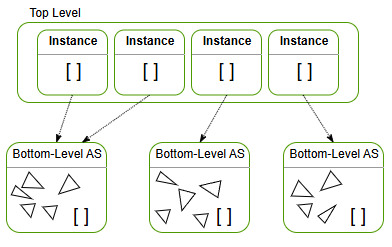
\includegraphics[width=0.5\textwidth]{pics/AccelerationStructure.png}
	\caption{Organizarea structurilor de accelerare în DXR~\protect\footnotemark}
	\label{fig:blas}
\end{figure}
\footnotetext{\copyright~\url{https://developer.nvidia.com/rtx/raytracing/dxr/dx12-raytracing-tutorial-part-1}. Accesat 24.06.2024.}

Framework-ul oferit de Microsoft~\cite{Schelet} oferă o structură minimală pentru
setup-ul unui proiect folosind DXR, precum crearea resurselor Direct3D, gestionarea
stărilor acestora și efectuarea pașilor descriși mai sus. Mare parte din acest
cod nu a fost modificat, cu excepția adăugării legăturilor pentru shaderele de
tip Ray Generation. De aceea, nu voi include cod legat de schelet în această secțiune,
ci mă voi concentra pe implementarea efectivă a algoritmului de Path Tracing din
cadrul HLSL.

\section{Meniul}
Meniul aplicației a fost creat folosind ImGui\footnote{\label{fn:imgui}\url{https://github.com/ocornut/imgui}. Accesat 24.06.2024.}, o bibliotecă open-source ce oferă
elementele de construcție pentru interfețe grafice imediate (care sunt integrate
în bucla de randare a aplicației). Pentru integrarea cu DirectX 12, ImGui oferă
un API minimal și ușor de folosit, însă am întampinat dificultăți. Conform documentației,
trebuie folosite simultan integrarea cu Win32 și cu DirectX 12. Operațiile de inițializare
și de curățare trebuie să se facă simultan. Totuși, dintr-un motiv necunoscut,
la recrearea resurselor de Direct3D, (împreună cu cele două contextele ale ImGui),
aplicația dă crash. Soluția găsită de mine a fost să dau shutdown doar la contextul
de Win32, iar după reinițializarea acestuia să repet aceeași secvență de restart
și pentru contextul de DirectX 12. Soluția se află în listarea~\ref{lst:imgui}.
\begin{lstlisting}[caption={Reinițializare ImGui. Bazat pe documentația oficială\protect\footref{fn:imgui}},label={lst:imgui},language=C++]
// Initialize imgui.
IMGUI_CHECKVERSION();
ImGui::CreateContext();
ImGuiIO& io = ImGui::GetIO();
io.ConfigFlags |= ImGuiConfigFlags_NavEnableKeyboard;

ImGui_ImplWin32_Init(Win32Application::GetHwnd());
D3D12_CPU_DESCRIPTOR_HANDLE cpuHandle;
UINT descriptorHeapIndex = AllocateDescriptor(&cpuHandle);

ImGui_ImplDX12_Shutdown();
ImGui_ImplDX12_Init(m_deviceResources->GetD3DDevice(),
	FrameCount,
	DXGI_FORMAT_R8G8B8A8_UNORM,
	m_descriptorHeap.Get(),
	cpuHandle,
	CD3DX12_GPU_DESCRIPTOR_HANDLE(m_descriptorHeap->GetGPUDescriptorHandleForHeapStart(),
		descriptorHeapIndex, m_descriptorSize));

ImGui::StyleColorsDark();
\end{lstlisting}

Meniul este modular. El poate fi redimensionat, mutat în cadrul ferestrei sau minimizat.
Secțiunile sunt grupate astfel:
\begin{itemize}
	\item \textbf{Header}: aici sunt afișate informații despre performanța aplicației,
	      precum FPS-ul, dar și timpul scurs și poziția camerei. Ilustrație în figura Figura~\ref{fig:imgui-controls}.
	\item \textbf{Controls}: aici sunt afișate controalele pentru aplicație.
	      Ilustrație în figura Figura~\ref{fig:imgui-controls}.
	\item \textbf{Renderer}: aici sunt afișate setările de configurare ale algoritmului
	      de randare, precum numărul de eșantioane, adâncimea maximă de recursivitate, etc.
	      Aici se pot configura și tehnicile de accelerare a convergenței definite în secțiunea~\ref{sec:options}.
	      Ilustrație în figura Figura~\ref{fig:imgui-renderer}.
	\item \textbf{Scene}: aici se pot configura luminile din scenă, precum culoarea de emisie,
	      tipul (de suprafață sau direcționale), intensitatea, direcția sau poziția.
	      Ilustrație în figura Figura~\ref{fig:imgui-scene}.
\end{itemize}

Codul utilizat pentru compunerea acestui meniu se află în listarea~\ref{lst:showui}.

\begin{figure}[!htb]
	\centering
	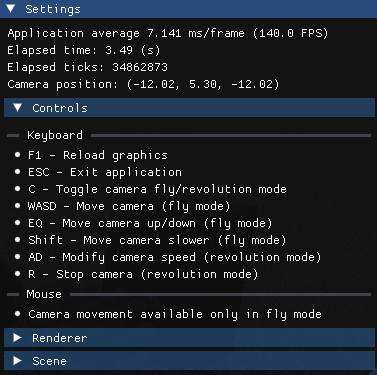
\includegraphics[width=0.5\textwidth]{pics/imgui-controls.png}
	\caption{Meniul aplicației, secțiunea de statistici și controale}
	\label{fig:imgui-controls}
\end{figure}
\begin{figure}[!htb]
	\centering
	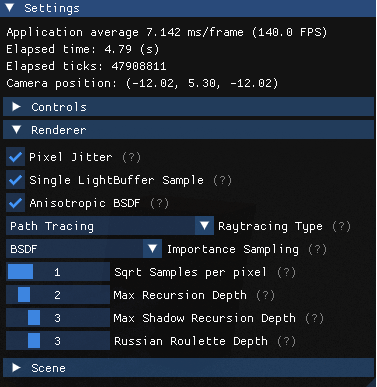
\includegraphics[width=0.5\textwidth]{pics/imgui-renderer.png}
	\caption{Meniul aplicației, secțiunea de configurare a algoritmului de randare}
	\label{fig:imgui-renderer}
\end{figure}
\begin{figure}[!htb]
	\centering
	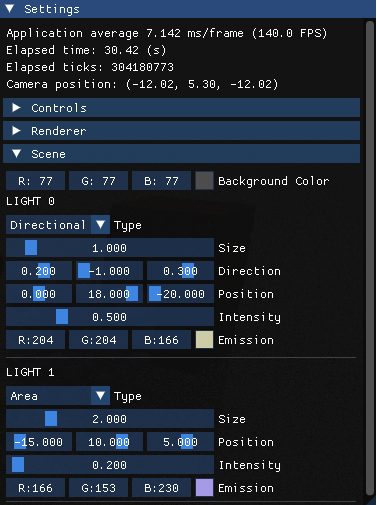
\includegraphics[width=0.5\textwidth]{pics/imgui-scene.png}
	\caption{Meniul aplicației, secțiunea de configurare a luminilor din scenă}
	\label{fig:imgui-scene}
\end{figure}

\section{Generator de numere aleatoare}

Natura algoritmului recursiv de tip Monte Carlo necesită un generator de numere
aleatoare care să fie rapid și să ofere o distribuție bună atât în lățime (deoarece
trebuie folosit de toți pixelii simultan) cât și în adâncime (deoarece trebuie
generate mai multe numere aleatoare per pixel). Am ales să folosesc un generator
PCG descris în~\cite{prng} care îndeplinește aceste cerințe (este și prng și hash). Codul
generatorului se află în listarea~\ref{lst:prng}.
\begin{lstlisting}[caption={Generatorul de numere aleatoare PCG\protect\footnotemark},label={lst:prng},language=C++]
// PRNG
// https://www.reedbeta.com/blog/hash-functions-for-gpu-rendering/
uint rand_pcg(inout uint rng_state)
{
	uint state = rng_state;
	rng_state = rng_state * 747796405u + 2891336453u;
	uint word = ((state >> ((state >> 28u) + 4u)) ^ state) * 277803737u;
	return (word >> 22u) ^ word;
}

float random(inout uint rng_state)
{
	return float(rand_pcg(rng_state)) / float(0xFFFFFFFFu);
}
\end{lstlisting}
\footnotetext{\url{https://www.reedbeta.com/blog/hash-functions-for-gpu-rendering/}. Accesat 24.06.2024.}

\section{Ray Generation shader}

Razele sunt generate în scenă pornind din fiecare pixel al imaginii. În funcție
de setări, se pot genera mai multe raze per pixel, pentru a obține o imagine
mai clară. Strategia de eșantionare este la bază stratificată și poate fi configurată,
putând fi activat sau dezactivat jittering-ul.

Pentru algoritmul normal de Path Tracing, se așteaptă să se calculeze
contribuția pentru fiecare eșantion și la final se stochează în buffer
media aritmetică a acestora. În schimb, pentru algoritmul progresiv, se
calculează contribuția pentru un singur eșantion și acumulează în buffer
folosind un factor de interpolare care asignează o pondere dependentă de
indexul eșantionului curent. Implementările pentru aceste rutine se află în
shadere de tip Ray Generation și sunt ilustrate în listările~\ref{lst:raygen} și~\ref{lst:raygen-progresiv}.

\begin{lstlisting}[caption={Generarea razelor în algoritmul Path Tracing},label={lst:raygen},language=C++]
[shader("raygeneration")] void RaygenShader_PathTracing()
{
	// Initialize the random number generator.
	uint rng_state = hash(DispatchRaysIndex().xy, g_sceneCB.elapsedTicks);

	float3 finalColor = float3(0.0f, 0.0f, 0.0f);

	uint numSamples = g_sceneCB.pathSqrtSamplesPerPixel * g_sceneCB.pathSqrtSamplesPerPixel;

	for (uint i = 0; i < g_sceneCB.pathSqrtSamplesPerPixel; i++)
		for (uint j = 0; j < g_sceneCB.pathSqrtSamplesPerPixel; j++)
		{
			// Compute the ray offset inside the pixel (for stratified sampling), between 0 and 1.
			float2 offset = numSamples == 1 ? float2(0.5f, 0.5f) : float2((i + 0.5f) / g_sceneCB.pathSqrtSamplesPerPixel, (j + 0.5f) / g_sceneCB.pathSqrtSamplesPerPixel);

			// Apply jittering if enabled.
			float2 jitter = select(g_sceneCB.applyJitter, float2(random(rng_state), random(rng_state)), float2(0.5f, 0.5f)); // in [0, 1)
			offset += (jitter - 0.5f) / g_sceneCB.pathSqrtSamplesPerPixel;

			// Generate a ray for a camera pixel corresponding to an index from the dispatched 2D grid.
			Ray ray = GenerateCameraRay(DispatchRaysIndex().xy, g_sceneCB.cameraPosition.xyz, g_sceneCB.projectionToWorld, offset);

			// Cast a ray into the scene and retrieve a shaded color.
			UINT currentRecursionDepth = 0;
			float4 color = TraceRadianceRay(ray, float4(1.0f, 1.0f, 1.0f, 1.0f), float4(0.0f, 0.0f, 0.0f, 0.0f), currentRecursionDepth);

			// Accumulate the color.
			finalColor += color.xyz;
		}

	// Average the accumulated color.
	g_renderTarget[DispatchRaysIndex().xy] = float4(finalColor / numSamples, 1.0f);
}
\end{lstlisting}

\begin{lstlisting}[caption={Generarea razelor în algoritmul Path Tracing progresiv},label={lst:raygen-progresiv},language=C++]
[shader("raygeneration")] void RaygenShader_PathTracingTemporal()
{
	// Initialize the random number generator.
	uint rng_state = hash(DispatchRaysIndex().xy, g_sceneCB.elapsedTicks);

	uint numSamples = g_sceneCB.pathSqrtSamplesPerPixel * g_sceneCB.pathSqrtSamplesPerPixel;

	// Compute the ray offset inside the pixel (for stratified sampling), between 0 and 1.
	float2 offset = numSamples == 1 ? float2(0.5f, 0.5f) : float2(((g_sceneCB.pathFrameCacheIndex - 1) % g_sceneCB.pathSqrtSamplesPerPixel + 0.5f) / g_sceneCB.pathSqrtSamplesPerPixel, (floor((g_sceneCB.pathFrameCacheIndex - 1) / g_sceneCB.pathSqrtSamplesPerPixel) + 0.5f) / g_sceneCB.pathSqrtSamplesPerPixel);

	// Apply jittering if enabled.
	float2 jitter = select(g_sceneCB.applyJitter, float2(random(rng_state), random(rng_state)), float2(0.5f, 0.5f)); // in [0, 1)
	offset += (jitter - 0.5f) / g_sceneCB.pathSqrtSamplesPerPixel;

	// Generate a ray for a camera pixel corresponding to an index from the dispatched 2D grid.
	Ray ray = GenerateCameraRay(DispatchRaysIndex().xy, g_sceneCB.cameraPosition.xyz, g_sceneCB.projectionToWorld, offset);

	// Cast a ray into the scene and retrieve a shaded color.
	UINT currentRecursionDepth = 0;
	float4 color = TraceRadianceRay(ray, float4(1.0f, 1.0f, 1.0f, 1.0f), float4(0.0f, 0.0f, 0.0f, 0.0f), currentRecursionDepth);

	// Accumulate the color.
	const float lerpFactor = 1.0f * (g_sceneCB.pathFrameCacheIndex - 1) / g_sceneCB.pathFrameCacheIndex;
	g_renderTarget[DispatchRaysIndex().xy] = float4(lerp(color.xyz, g_renderTarget[DispatchRaysIndex().xy].xyz, lerpFactor), 1.0f);
}
\end{lstlisting}

\section{Closest Hit shader}
Sunt două shadere de acest tip - unul pentru primitive și unul pentru suprafețele bounding box-urile
suprafețelor implicite și analitice. Ambele apelează aceeași funcție helper care alege
dintre algoritmul de Ray Tracing Whitted și Path Tracing pentru a calcula reflectanța în punctul
de intersecție. Iluminarea pentru Ray Tracing era deja implementată în schelet, așa că nu o mai
includem. Codul pentru Path Tracing este ilustrat în listarea~\ref{lst:closesthit}.
\begin{lstlisting}[caption={Closest Hit helper pentru Path Tracing},label={lst:closesthit},language=C++]
void ClosestHitHelper(inout RayPayload rayPayload, in float3 normal, in float3 hitPosition)
{
	float4 color = float4(0.0f, 0.0f, 0.0f, 1.0f);
	if (g_sceneCB.raytracingType > 0) // path tracing
	{
		color.xyz = DoPathTracing(rayPayload, l_pbrCB, normal, hitPosition, RayTCurrent());
	}
	else // Whitted-style ray tracing
	{
		// Reflected component.
		// color.xyz = ...
	}

	// Apply visibility falloff.
	float t = RayTCurrent();
	color = lerp(color, g_sceneCB.backgroundColor, 1.0 - exp(-0.000002 * t * t * t));

	rayPayload.color = color;
}
\end{lstlisting}

\subsection{Algoritmul Path Tracing}
Funcția \texttt{DoPathTracing} definește întreg algoritmul de Path Tracing. Aici
se efectuează toate optimizările și tehnicile de accelerare a convergenței
despre care am vorbit în capitolul~\ref{sec:solutie}. Listarea~\ref{lst:pathtracing}
ilustrează implementarea algoritmului.

Observăm la liniile \ref{line:absorption1},~\ref{line:absorption2} și~\ref{line:absorption3}
prezența unui termen de absorbție. Acesta modelează absorbția volumetrică a luminii
când parcurge un mediu. Acesta se aplică doar în cazul în care raza se află
în interiorul unui obiect. Modelul este bazat pe legea Beer-Lambert:
\begin{equation}\label{eq:absorption}
	T = e^{-\sigma_a d},
\end{equation}
unde $T$ reprezintă coeficientul de transmisie, $\sigma_a$ este coeficientul de absorbție,
iar $d$ este distanța parcursă în interiorul obiectului.
Pentru parametrizare în cadrul materialului, am introdus 2 noi parametri: $atDistance$ și
$extinction$. Inversând ecuația~\ref{eq:absorption}, putem obține coeficientul de absorbție:
\begin{equation}
	\sigma_a = -\dfrac{\log(extinction)}{atDistance}.
\end{equation}

Funcțiile \texttt{MIS} și \texttt{NextEventEstimation} sunt folosite pentru eșantionarea
multiplă bazată pe importanță. Acestea sunt implementate conform teoriei prezentate în
capitolul~\ref{sec:stateoftheart}. Codul pentru aceste funcții se află în listarea~\ref{lst:mis}.
\begin{lstlisting}[caption={Funcțiile de eșantionare multiplă bazată pe importanță},label={lst:mis},language=C++]
// Samples a light source.
bool NextEventEstimation(inout uint rng_state, in LightBuffer light, in float3 hitPosition,
								in uint recursionDepth, out LightSample lightSample)
{
	float angle;
	float2 eps;
	float3 samplePos;
	switch (light.type)
	{
	case LightType::Square:
		eps = float2(random(rng_state), random(rng_state));
		samplePos = light.position + float3(eps.x - 0.5f, 0.0f, eps.y - 0.5f) * light.size;
		lightSample.L = samplePos - hitPosition;
		lightSample.dist = length(lightSample.L);
		lightSample.L /= lightSample.dist;
		// bail out if the sample is on the wrong side of the light
		angle = dot(lightSample.L, float3(0.0f, 1.0f, 0.0f));
		if (angle <= 0.0f)
			return false;
		lightSample.emission = light.intensity * light.emission;
		lightSample.pdf = (sq(lightSample.dist)) / (sq(light.size) * angle);
		break;
	case LightType::Directional:
		lightSample.L = -normalize(light.direction);
		lightSample.dist = INFINITY;
		lightSample.emission = light.intensity * light.emission;
		lightSample.pdf = 1.0f;
		break;
	}

	// Check if the light is occluded.
	Ray shadowRay = {hitPosition, lightSample.L};
	bool shadowRayHit = recursionDepth < g_sceneCB.maxShadowRecursionDepth && TraceShadowRayAndReportIfHit(shadowRay, recursionDepth);
	return !shadowRayHit;
}

float3 MIS(inout uint rng_state, PBRPrimitiveConstantBuffer material, in float eta,
	in float3 hitPosition, in LightBuffer light, in float3 N, in uint recursionDepth)
{
	float3 reflectance = float3(0.0f, 0.0f, 0.0f);

	// Sample the light source.
	LightSample lightSample;
	if (NextEventEstimation(rng_state, light, hitPosition, recursionDepth, lightSample))
	{
		// Evaluate the BSDF.
		float bsdfPdf;
		reflectance = EvaluateDisneyBSDF(material, g_sceneCB.anisotropicBSDF, eta, -WorldRayDirection(), lightSample.L, N, bsdfPdf);

		// Calculate the MIS weight.
		float weight = 1.0f;
		if (light.type != LightType::Directional)
			weight = PowerHeuristic(1.0f, lightSample.pdf, 1.0f, bsdfPdf);

		// Calculate the final color.
		if (bsdfPdf > 0.0f)
			reflectance *= weight * lightSample.emission / lightSample.pdf;
		else
			reflectance = float3(0.0f, 0.0f, 0.0f);
	}

	return reflectance;
}
\end{lstlisting}

\section{Miss shader}

În cazul în care o rază nu intersectează niciun obiect din scenă, se execută
shader-ul de tip Miss. Acesta adaugă culoarea de fundal drept contribuție la cale (vezi listarea~\ref{lst:miss}).
\begin{lstlisting}[caption={Shader-ul de tip Miss},label={lst:miss},language=C++]
[shader("miss")] void MissShader(inout RayPayload rayPayload)
{
	rayPayload.color = g_sceneCB.backgroundColor * rayPayload.throughput;
}
\end{lstlisting}

\section{Evaluarea și eșantionarea BSDF-ului}

În secțiunile ~\ref{sec:pbr} și~\ref{sec:disney} am prezentat bazele teoretice
ale funcțiilor de distribuție a reflectanței și am prezentat modelul Disney Principled
BSDF. Totuși, nu am vorbit despre eșantionarea acestora. Acesta este un proces complex
și de obicei nu se găsesc soluții analitice. Astfel, diferite implementări folosesc
diferite metode de eșantionare și asignează ponderi diferite lobilor. Totuși, ideea
de bază este aceeași: pentru evaluare, se evaluează toți lobii (care au sens - nu evaluăm
transmisia dacă avem reflexie) și se ponderează în funcție de parametrii materialului,
pentru a asigna un fel de probabilitate ad-hoc fiecărui lob. Pentru eșantionare
(alegerea direcției razei următoare), se alege probabilistic (folosind aceleași ponderi
ca la evaluare) un singur lob și se eșantionează conform unei distribuții bazate
pe importanță ce aproximează cât mai bine distribuția microfațetelor din cadrul BRDF-ului.

În implementare am urmat modelul de eșantionare folosit în~\cite{GlslPathTracer}.
Codul se află în listarea~\ref{lst:bsdf}. Vreau să subliniez faptul că mi-a fost foarte
greu să ajung la o implementare corectă a BSDF-ului, din cauza complexității matematice.

\chapter{\label{sec:evaluare}Evaluare}

\section{Evaluarea performanțelor}

În continuare prezentăm rezultatele obținute în urma testelor de performanță. Toate
testele folosesc aceeași scenă și aceeași poziționare a camerei (ca în Figura~\ref{fig:demo_pathtracing}), astfel încât să se
observe impactul fiecărei setări asupra performanței. Vom varia pe rând fiecare setare,
ținând restul constante. Valorile implicite ale setărilor sunt:
\begin{itemize}
	\item Numărul de eșantioane per pixel: 2
	\item Adâncimea maximă de recursivitate: 2
	\item Adâncimea minimă pentru ruleta rusească: 3
	\item O singură lumină eșantionată: adevărat
	\item Metodă de eșantionare a direcției următoare: BSDF.
\end{itemize}

Rezultatele sunt prezentate în tabelele următoare. Testele au fost efectuate la o
rezoluție de 1920x1080 pixeli, pe o placă video Nvidia RTX 2060 Super. Menționăm
faptul că FPS-urile sunt limitate la 140.

\subsection{Numărul de eșantioane per pixel}
\begin{table}[!bth]\small\linespread{1}
	\centering
	\caption{Performanța în funcție de numărul de eșantioane per pixel}
	\begin{tabular}{l >{\raggedright\arraybackslash}p{4cm} >{\raggedright\arraybackslash}p{2cm}}
		\textbf{Valoare Setată} & \textbf{FPS} \\\hline
		\textbf{1}              & 75           \\\hline
		\textbf{4}              & 16           \\\hline
		\textbf{8}              & 6            \\\hline
		\textbf{16}             & 1            \\\hline
	\end{tabular}
	\label{tab:samples}
\end{table}
Rezultatele din tabela~\ref{tab:samples} arată că numărul de eșantioane per pixel
are un impact imens asupra performanței. Un număr modest de 4 eșantioane per pixel
nu este totuși suficient pentru a crea o imagine stabilă în absența tehnicilor
de denoising, așadar algoritmul este limitat în acest aspect.

\subsection{Adâncimea maximă a recursivității}
\begin{table}[!bth]\small\linespread{1}
	\centering
	\caption{Performanța în funcție de numărul de adâncimea maximă a recursivității}
	\begin{tabular}{l >{\raggedright\arraybackslash}p{4cm} >{\raggedright\arraybackslash}p{2cm}}
		\textbf{Valoare Setată} & \textbf{FPS} \\\hline
		\textbf{1}              & 140          \\\hline
		\textbf{2}              & 77           \\\hline
		\textbf{3}              & 40           \\\hline
		\textbf{4}              & 36           \\\hline
		\textbf{5}              & 33           \\\hline
		\textbf{6}              & 32           \\\hline
		\textbf{7}              & 31           \\\hline
		\textbf{8}              & 31           \\\hline
		\textbf{9}              & 30           \\\hline
		\textbf{10}             & 29           \\\hline
	\end{tabular}
	\label{tab:depth}
\end{table}
Rezultatele din tabela~\ref{tab:depth} arată că adâncimea maximă a recursivității
are și ea un impact semnificativ asupra performanței. Pentru a avea reflexii convingătoare,
o adâncime de 3 este suficientă, pe când în cazul refracțiilor, o adâncime de 5 este
ma potrivită. Observăm totuși că impactul scade odată cu creșterea adâncimii, ceea ce
este un efect al ruletei rusești.

\subsection{Adâncimea minimă pentru ruleta rusească}
\begin{table}[!bth]\small\linespread{1}
	\centering
	\caption{Performanța în funcție de adâncimea minimă la care se aplică ruleta rusească. Pentru acest test s-a setat adâncimea maximă de recursivitate la 10}
	\begin{tabular}{l >{\raggedright\arraybackslash}p{4cm} >{\raggedright\arraybackslash}p{2cm}}
		\textbf{Valoare Setată} & \textbf{FPS} \\\hline
		\textbf{1}              & 35           \\\hline
		\textbf{2}              & 34           \\\hline
		\textbf{3}              & 34           \\\hline
		\textbf{4}              & 32           \\\hline
		\textbf{5}              & 32           \\\hline
		\textbf{6}              & 31           \\\hline
		\textbf{7}              & 31           \\\hline
		\textbf{8}              & 30           \\\hline
		\textbf{9}              & 30           \\\hline
		\textbf{10}             & 29           \\\hline
	\end{tabular}
	\label{tab:roulette}
\end{table}
Tabela~\ref{tab:roulette} arată că ruleta rusească este o metodă destul de eficientă
pentru a crește performanța de rulare, fără a sacrifica prea mult calitatea imaginii.

\subsection{Eșantionarea unei singure lumini}
\begin{table}[!bth]\small\linespread{1}
	\centering
	\caption{Performanța în eșantionarea unei singure lumini sau a amândurora}
	\begin{tabular}{l >{\raggedright\arraybackslash}p{4cm} >{\raggedright\arraybackslash}p{2cm}}
		\textbf{Valoare Setată} & \textbf{FPS} \\\hline
		\textbf{DA}             & 87           \\\hline
		\textbf{NU}             & 77           \\\hline
	\end{tabular}
	\label{tab:onelight}
\end{table}
Tabela~\ref{tab:onelight} arată că eșantionarea unei singure lumini are un impact
bun asupra performanței, fără a sacrifica deloc calitatea imaginii. Acest test s-a
efectuat cu doar 2 lumini în scenă - scene mai complexe vor avea un impact imens
asupra performanței dacă se eșantionează toate luminile deodată (spre deosebire
de niciun impact în setarea cealaltă, însă asta aduce o reducere a calității imaginii).

\subsection{Strategia de eșantionare a direcției următoare}
\begin{table}[!bth]\small\linespread{1}
	\centering
	\caption{Performanța în funcție de strategia de eșantionare a direcției următoare}
	\begin{tabular}{l >{\raggedright\arraybackslash}p{4cm} >{\raggedright\arraybackslash}p{2cm}}
		\textbf{Valoare Setată}             & \textbf{FPS} \\\hline
		\textbf{BSDF}                       & 87           \\\hline
		\textbf{Cosine-weighted Hemisphere} & 51           \\\hline
		\textbf{Uniform sphere}             & 46           \\\hline
	\end{tabular}
	\label{tab:bsdf}
\end{table}
Tabela~\ref{tab:bsdf} arată că eșantionarea bazată pe BSDF este, surprinzător, cea mai eficientă
dar și cea mai calitativă (vezi Figurile~\ref{fig:eval-bsdf}, \ref{fig:eval-cosine} și \ref{fig:eval-uniform}). Presupunerea mea este că, deoarece podeaua are un material specular,
eșantionarea BSDF-ului va conduce rapid la ieșirea razelor din scenă și la oprirea
recursivității. Eșantionarea uniformă a sferei este cea mai lentă, deoarece implică și
o componentă de transmisie.

\section{Evaluare calitativă}

\subsection{Comparație cu Ray Tracing Whitted}

Algoritmul integrat deja în schelet este un Ray Tracer recursiv simplu, de tip Whitted,
care folosește un model de iluminare Phong. Acesta nu suportă transmisie, iar
reflexiile sunt perfect geometrice. O randare realizată cu acest algoritm se poate
vedea în Figura~\ref{fig:demo_whitted}. Torusul de tip inel și cele 3 sfere
au un material ce simulează cromul și este reflectiv. Se pot observa și umbre
geometrice, cauzate de două surse de lumină punctiforme.
\begin{figure}[ht]
	\centering
	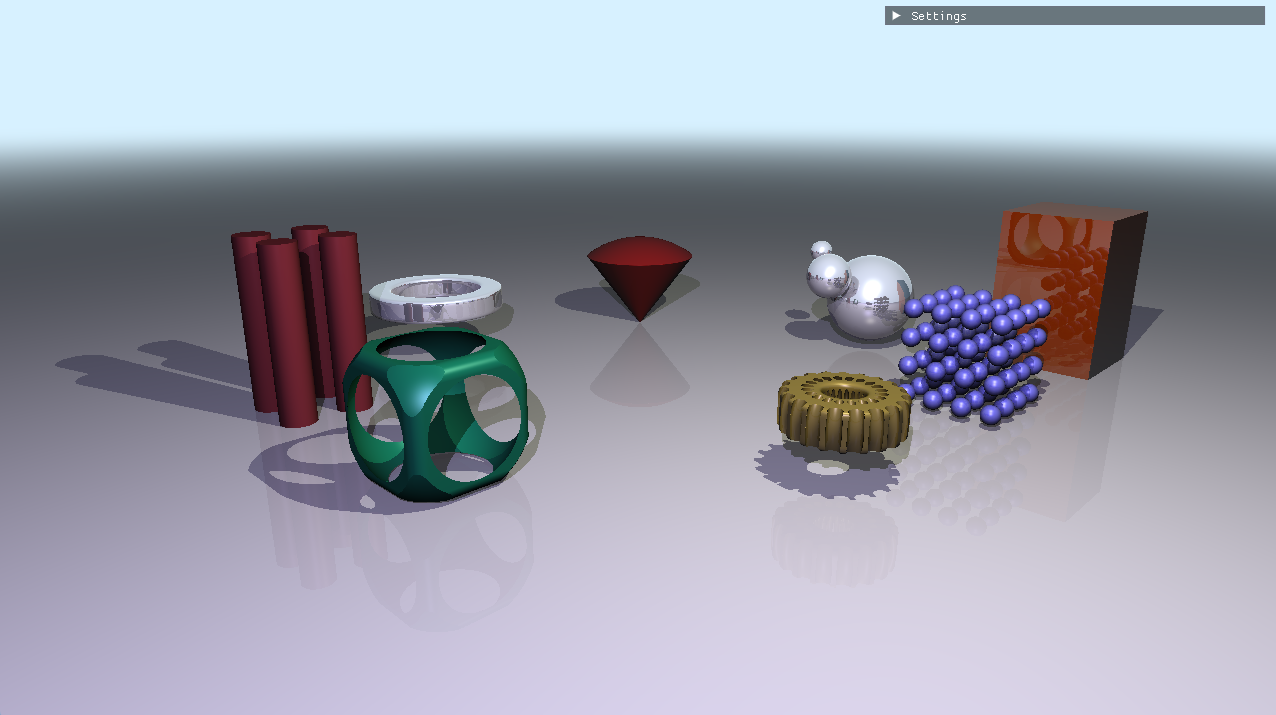
\includegraphics[width=\textwidth]{pics/demo_whitted.png}
	\caption{Randare folosing Ray Tracing Whitted}
	\label{fig:demo_whitted}
\end{figure}
Aceeași scenă, dar randată folosind Path Tracing, se poate vedea în Figura~\ref{fig:demo_pathtracing}.
Condițiile de iluminare nu pot fi replicate perfect. Observăm imediat o diferență
majoră - această randare ține cont de iluminarea globală. Scena este iluminată
conform fundalului, iar contribuția reflectanței fiecărui obiect este vizibilă
pe podea. În acest caz, lumina nu este destul de puternică să lupte cu fundalul,
de aceea umbrele sunt destul de puțin pronunțate. În randarea din Figura~\ref{fig:demo_pathtracing2}
culoarea de fundal a fost coborâtă - se observă astfel contribuțiile celor două surse
de lumină - una de tip suprafață și una direcțională. Umbrele lăsate de zonele
obstrucționate din perspectiva luminii de suprafață au un aspect natural, cu penumbre
ce tranziționează lin între umbra completă și lumina directă.
\begin{figure}[!htb]
	\centering
	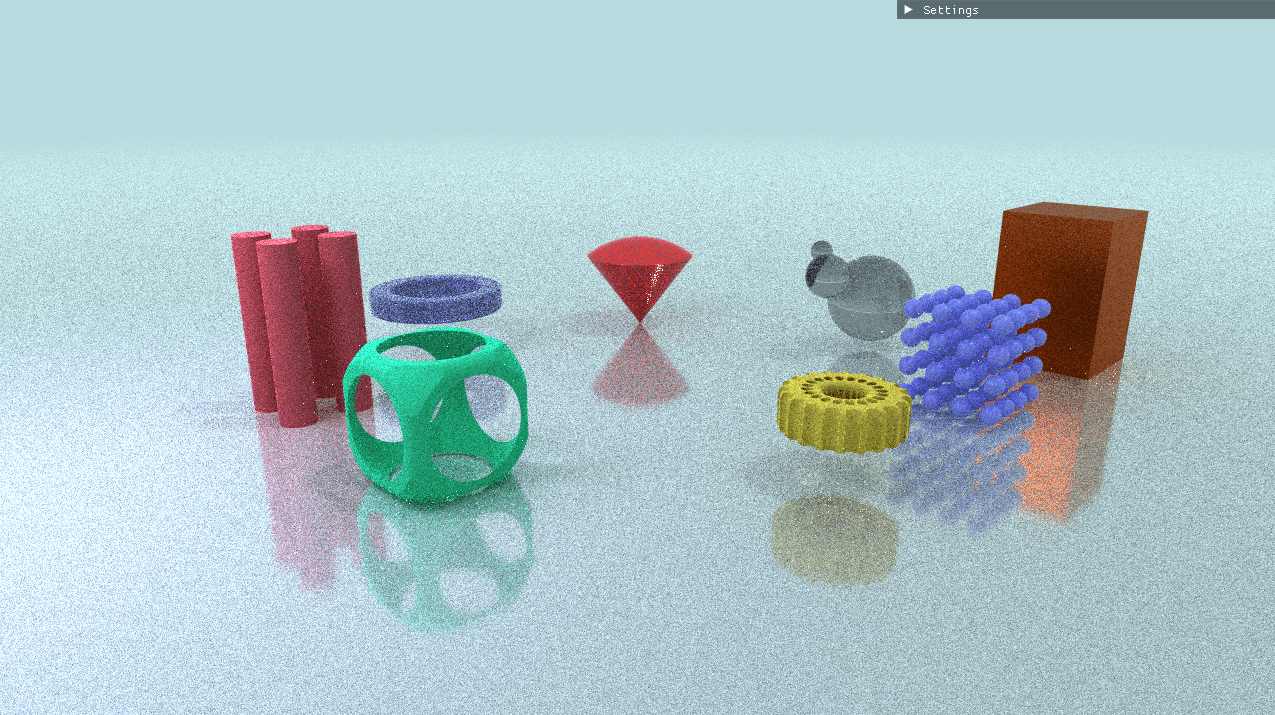
\includegraphics[width=\textwidth]{pics/demo_pathtracing.png}
	\caption{Randare folosind Path Tracing}
	\label{fig:demo_pathtracing}
\end{figure}
\begin{figure}[!htb]
	\centering
	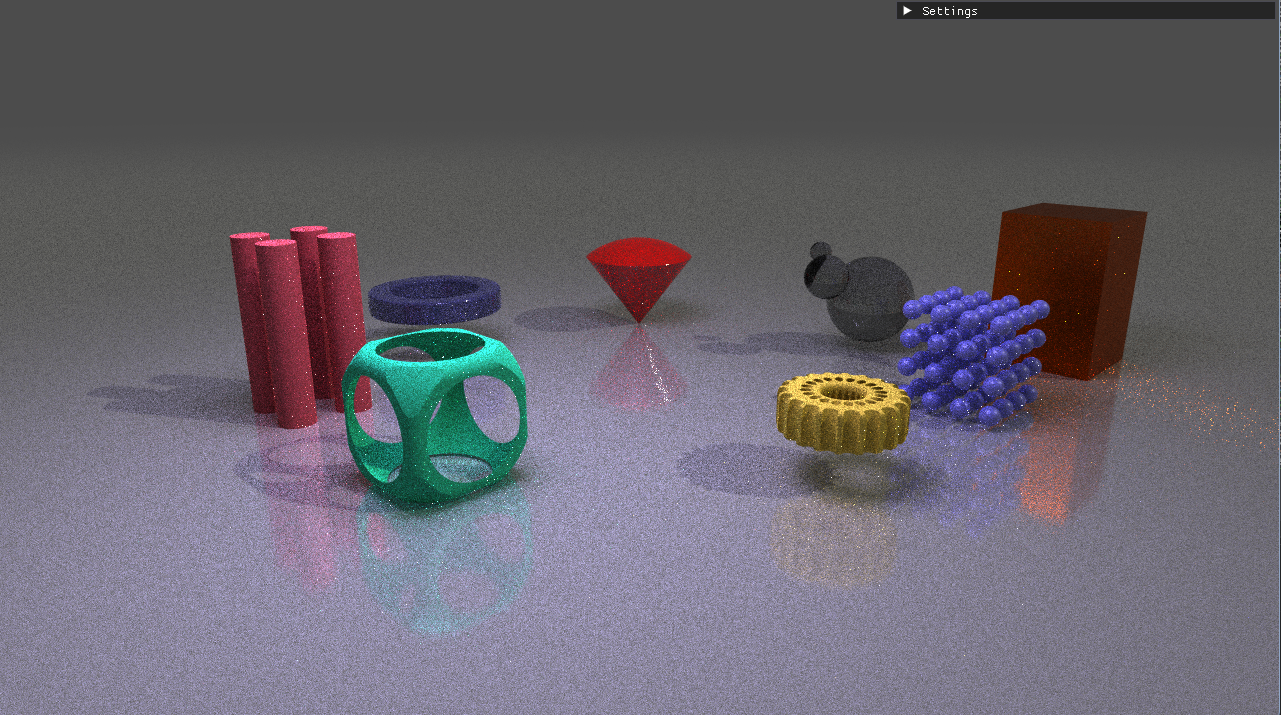
\includegraphics[width=\textwidth]{pics/demo_pathtracing2.png}
	\caption{Randare folosind Path Tracing cu fundal mai întunecat}
	\label{fig:demo_pathtracing2}
\end{figure}

Așa cum este descris în secțiunea~\ref{sec:disney}, sistemul de materiale
folosit este physically based și modelează efecte complexe precum reflexii și
refracții. Un exemplu de material care dă dovadă de ambele comportamente se află
în figura Figura~\ref{fig:demo_refraction}. Acesta este un material dielectric, cu
un indice de refracție de 1.5. Se observă refracții către obiectele din spate
în zonele centrale ale sferelor și reflexii către mediul înconjurător către
margini, unde unghiul de incidență este mare. Acest comportament este consistent
cu legile lui Fresnel.
\begin{figure}[!htb]
	\centering
	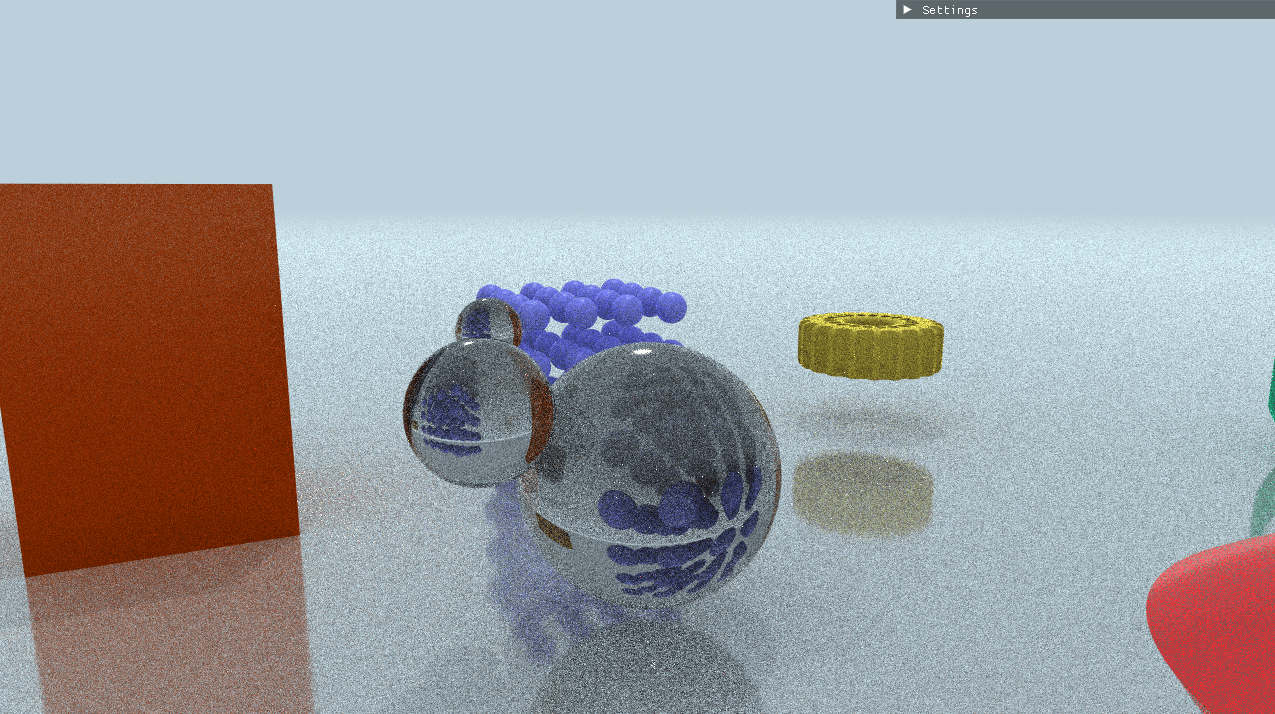
\includegraphics[width=\textwidth]{pics/demo_refraction.png}
	\caption{Randare folosind Path Tracing cu sticlă dielectrică}
	\label{fig:demo_refraction}
\end{figure}

\subsection{Evaluarea strategiei de eșantionare a direcției următoare}

Așa cum era de așteptat, eșantionarea bazată pe importanța BSDF-ului converge cel mai repede.
Celelalte strategii nu reușesc să conveargă nici la 256 eșantioane per pixel, în timp ce
imaginea eșantionată cu BSDF este foarte stabilă. Ilustrații în Figurile~\ref{fig:eval-bsdf},
\ref{fig:eval-cosine} și~\ref{fig:eval-uniform} arată această diferență.

\begin{figure}[!htb]
	\centering
	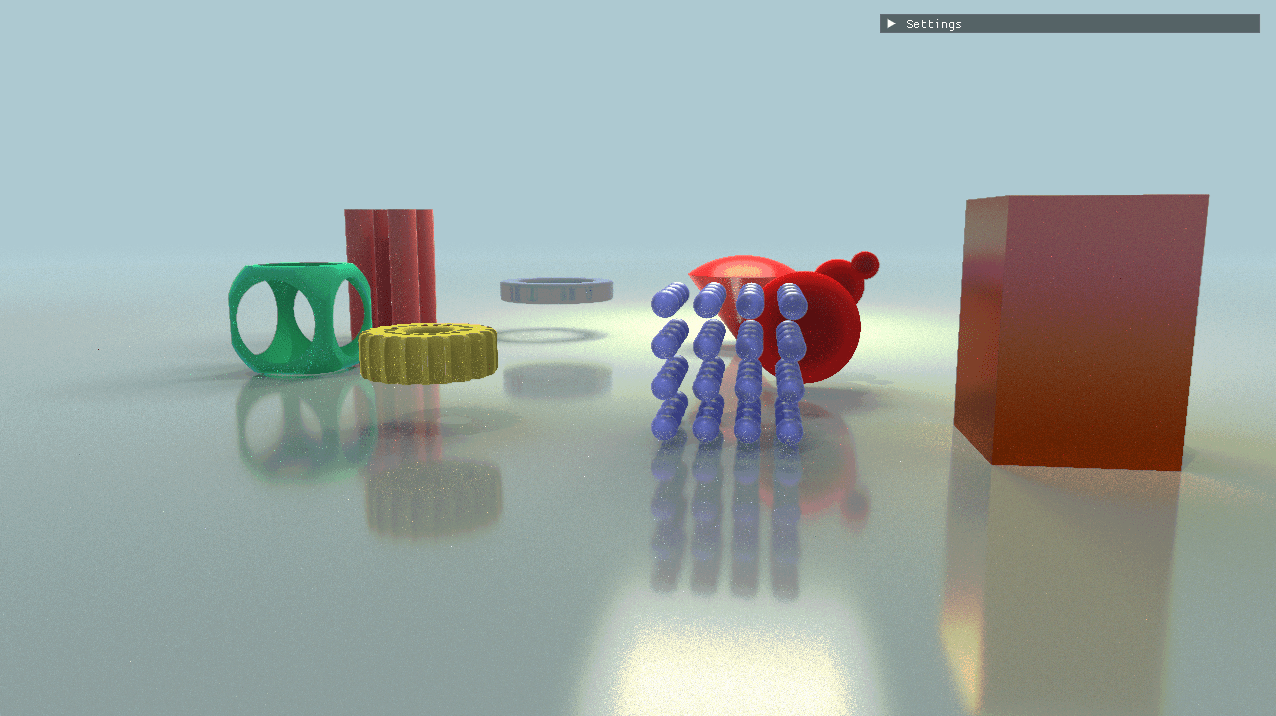
\includegraphics[width=\textwidth]{pics/demo-bsdf.png}
	\caption{Eșantionare bazată pe BSDF}
	\label{fig:eval-bsdf}
\end{figure}
\begin{figure}[!htb]
	\centering
	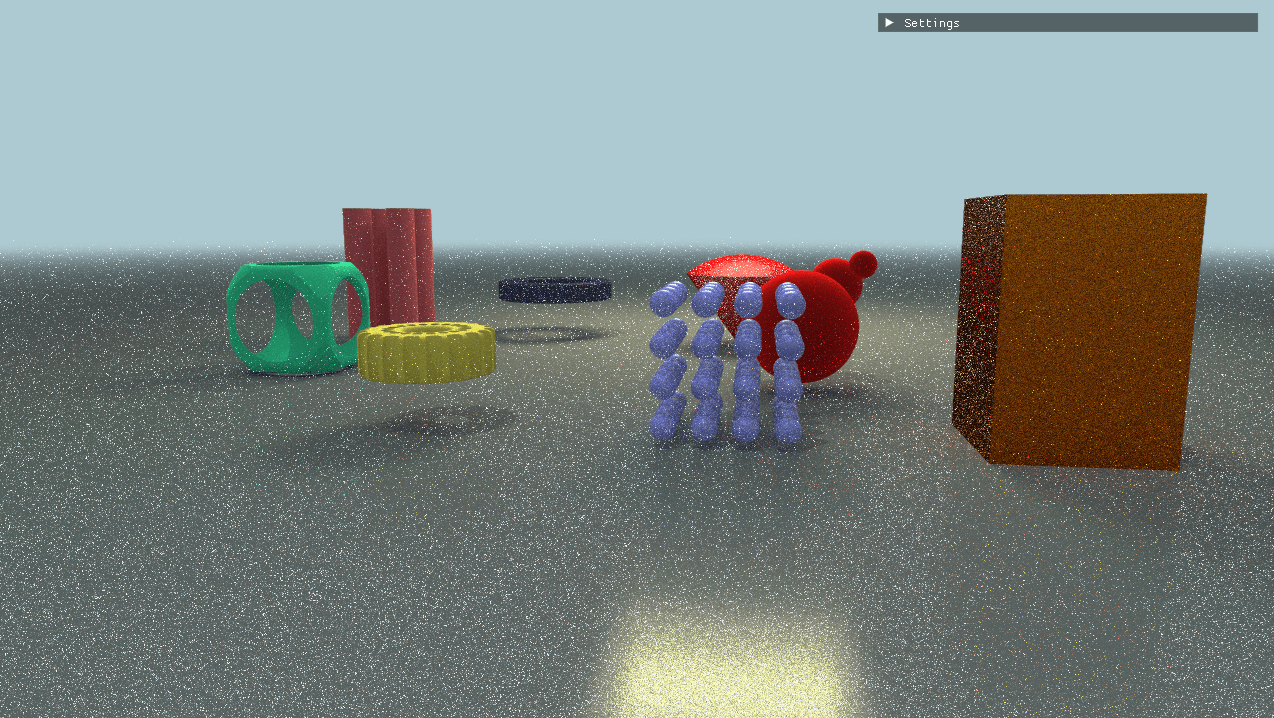
\includegraphics[width=\textwidth]{pics/demo-cosine.png}
	\caption{Eșantionare ponderată de cosinus a emisferei}
	\label{fig:eval-cosine}
\end{figure}
\begin{figure}[!htb]
	\centering
	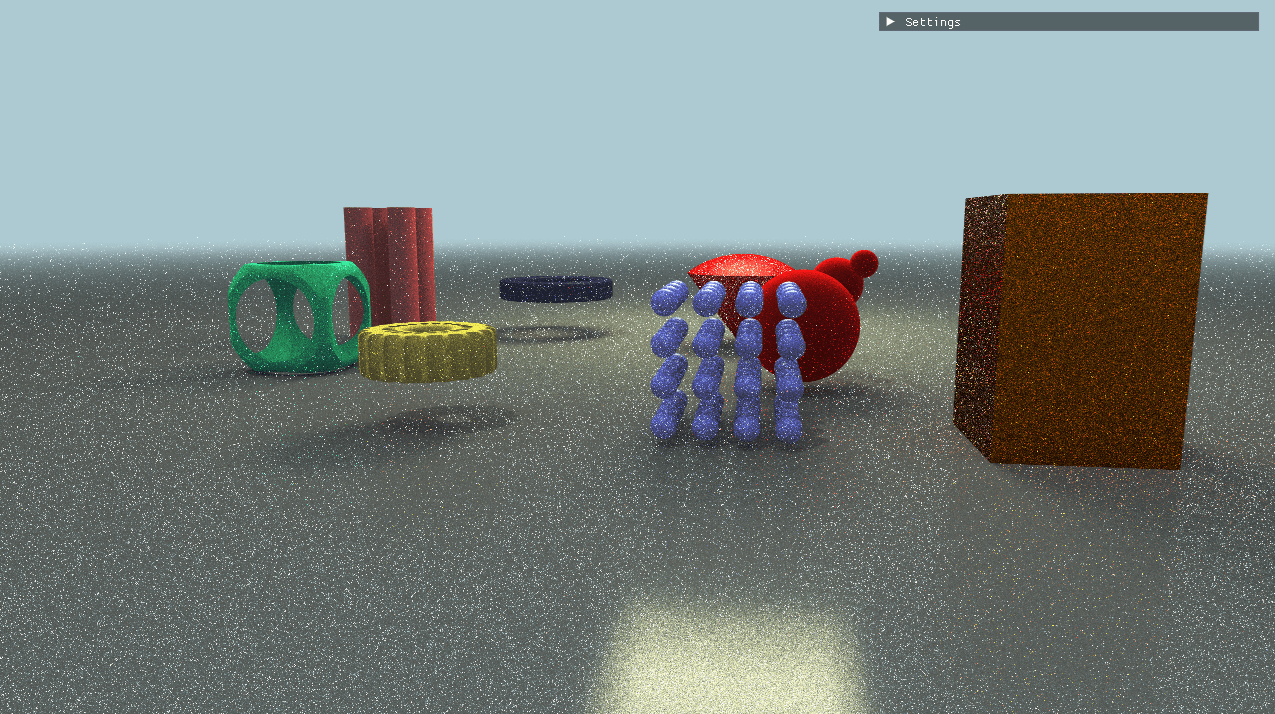
\includegraphics[width=\textwidth]{pics/demo-uniform.png}
	\caption{Eșantionare uniformă a sferei}
	\label{fig:eval-uniform}
\end{figure}


\subsection{Evaluarea modelului Disney principled BSDF}

Am descris în secțiunea~\ref{sec:disney} modelul Disney principled BSDF, modelul
de materiale folosit în această implementare. Acesta este un model complex dar foarte bun,
folosit în producție la Disney pentru filmele lor animate încă din anul 2012~\cite{Disney}.
Vom supune așadar acest model la teste pentru a ne convinge de calitatea și fidelitatea sa. 

În continuare, vom evalua efectele parametrilor care definesc sistemul de materiale. Pentru această
scenă s-au folosit setările la calitate maximă: 256 eșantioane per pixel, algoritm progresiv și adâncime
maximă de recursivitate 10. Am folosit pentru aceste randări varianta progresivă a algoritmului,
pentru a obține performanțe comparabile cu un singur eșantion per pixel dar calitate mult mai bună.
În următoarele randări, s-a variat câte un parametru
în timp ce restul sunt la valorile implicite (i.e., 0 pentru majoritatea și 1.5 pentru
indexul de refracție)

\begin{figure}[!htb]
	\centering
	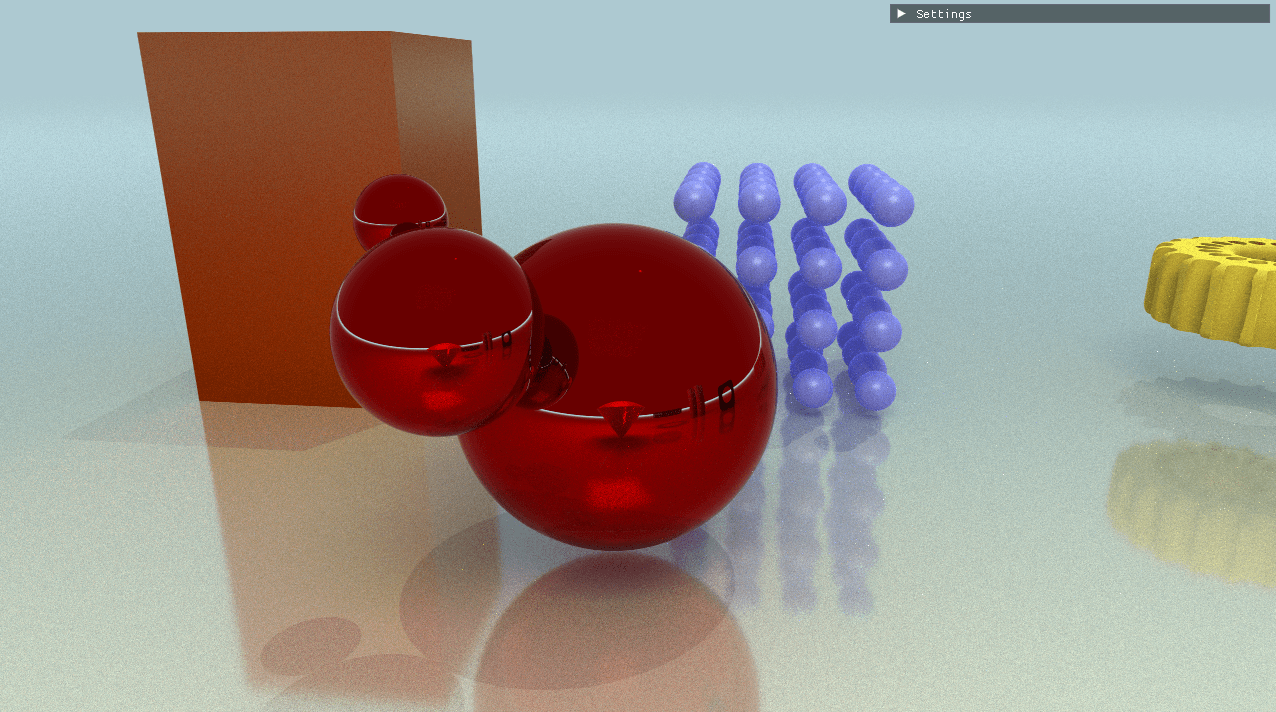
\includegraphics[width=\textwidth]{pics/demo-metallic-1.0.png}
	\caption{Material metallic cu $metallic = 1.0$. Se pot observa reflexiile speculare
		ce sunt colorate în funcție de culoarea materialului}
	\label{fig:demo-metallic-1.0}
\end{figure}
\begin{figure}[!htb]
	\centering
	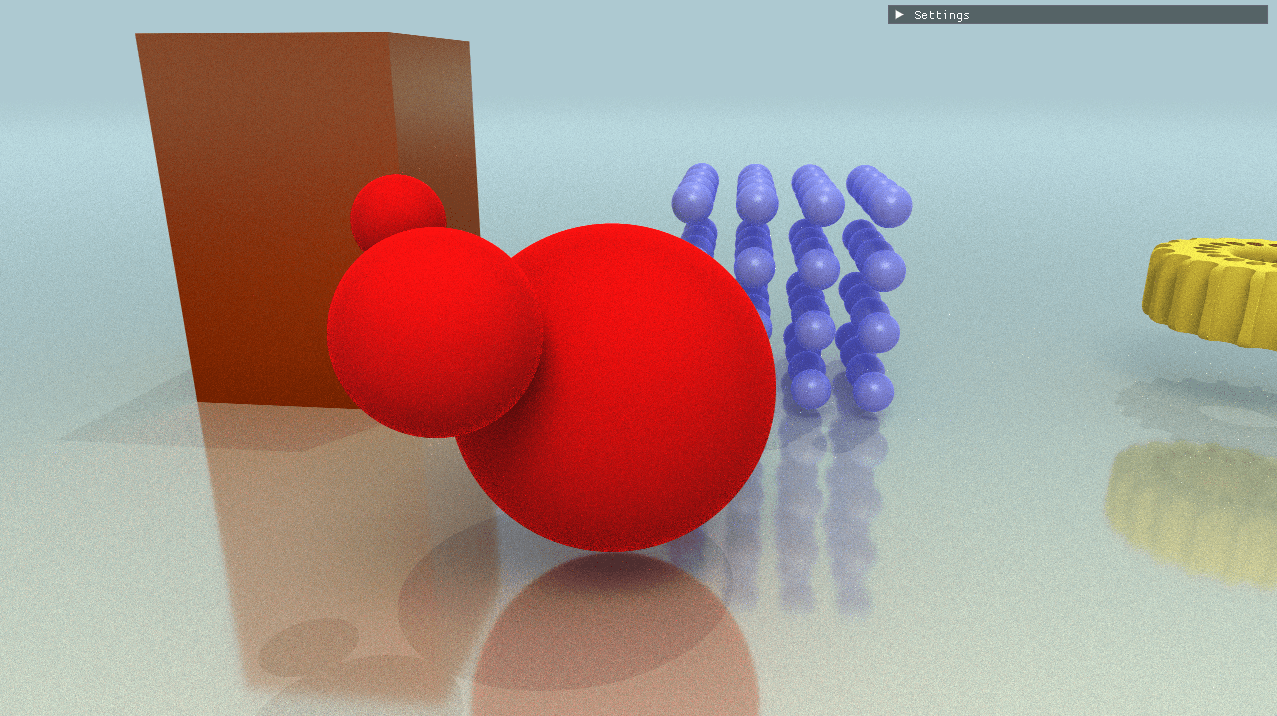
\includegraphics[width=\textwidth]{pics/demo-rough-1.0.png}
	\caption{Material dielectric cu $roughness = 1.0$. Se observă modelul difuz}
	\label{fig:demo-rough-1.0}
\end{figure}
\begin{figure}[!htb]
	\centering
	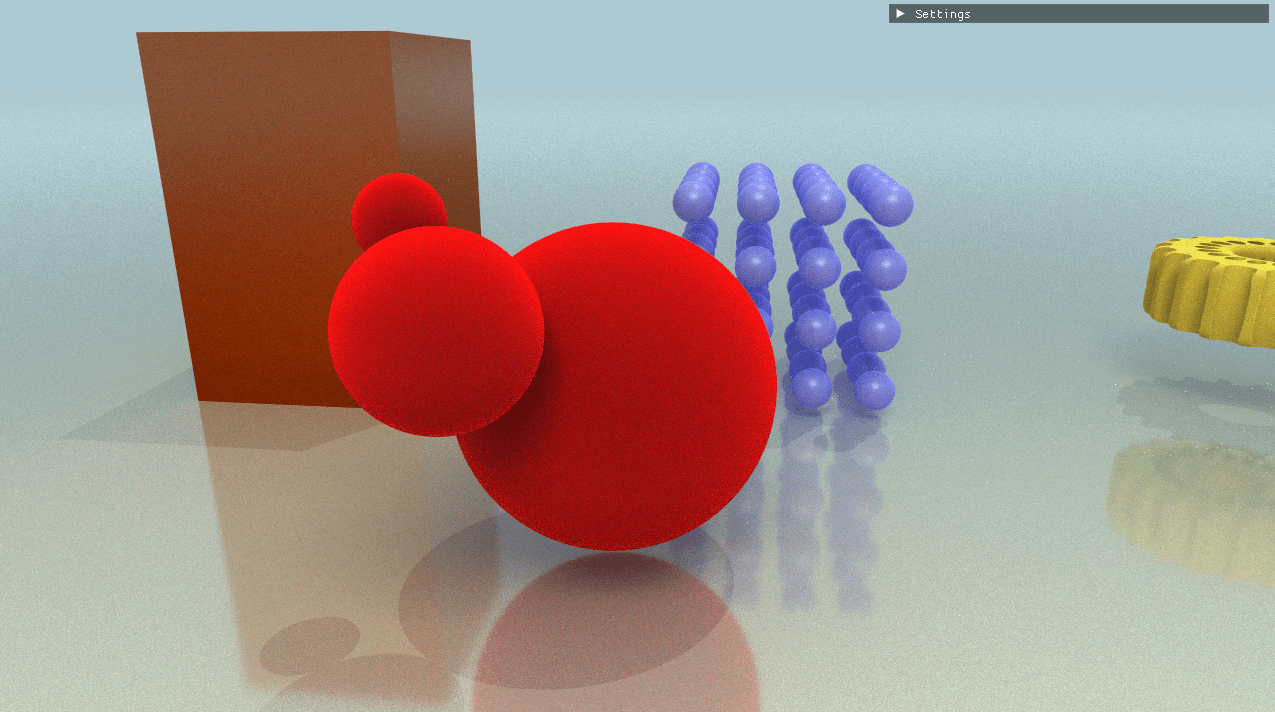
\includegraphics[width=\textwidth]{pics/demo-subsurface-1.0.png}
	\caption{Material dielectric cu $subsurface = 1.0$ și $roughness = 0.0$. Se observă modelul difuz și efectul de subsurface scattering}
	\label{fig:demo-subsurface-1.0}
\end{figure}
\begin{figure}[!htb]
	\centering
	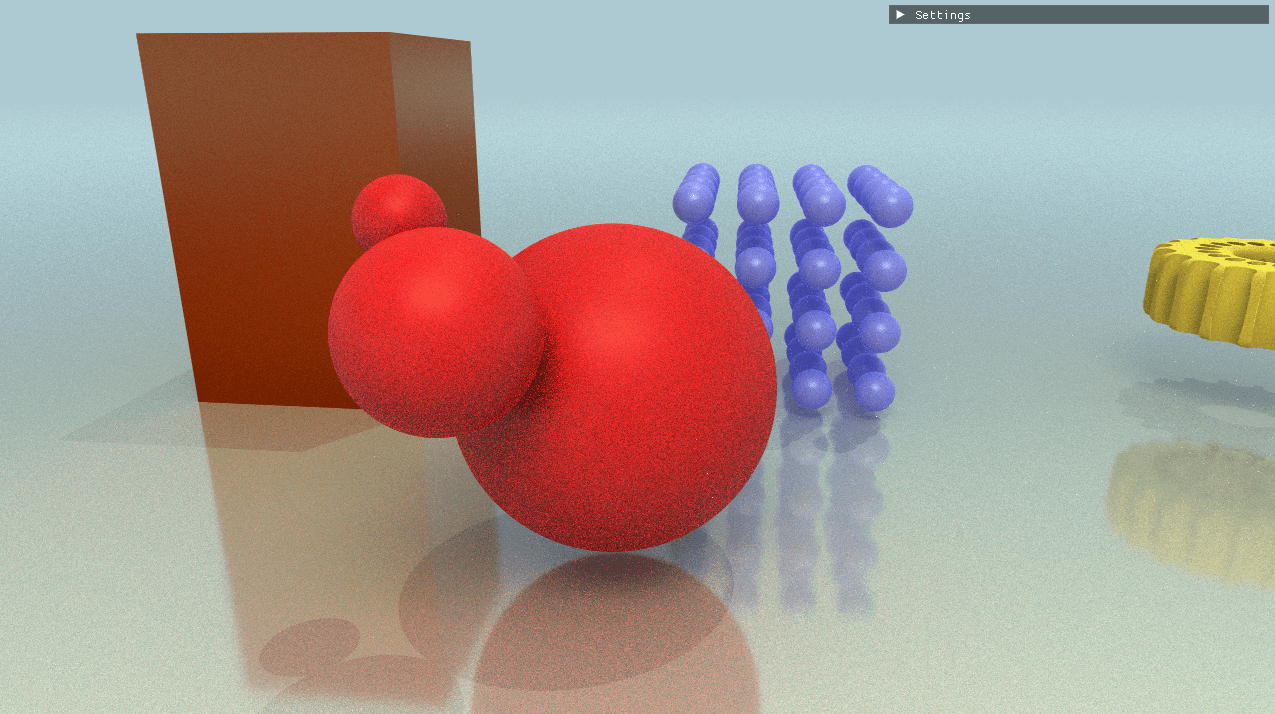
\includegraphics[width=\textwidth]{pics/demo-clearcoat-1.0.png}
	\caption{Material cu strat de clearcoat cu $clearcoat = 1.0$ și $roughness = 0.5$. Se observă un luciu
		adițional (deși minor) pe material}
	\label{fig:demo-clearcoat-1.0}
\end{figure}
\begin{figure}[!htb]
	\centering
	\includegraphics[width=\textwidth]{pics/demo-clearcoatGloss-1.0.png}
	\caption{Material dielectric cu $clearcoat = 1.0,\ clearcoatGloss = 1.0$ și $roughness = 0.5$. Se observă efectul de luciu pronunțat}
	\label{fig:demo-clearcoatGloss-1.0}
\end{figure}
\begin{figure}[!htb]
	\centering
	\includegraphics[width=\textwidth]{pics/demo-anisotropy-1.0.png}
	\caption{Material dielectric cu $anisotropy = 1.0$ și $roughness = 0.5$. Se observă anizotropia punctelor speculare}
	\label{fig:demo-anisotropy-1.0}
\end{figure}
\begin{figure}[!htb]
	\centering
	\includegraphics[width=\textwidth]{pics/demo-sheen-1.0.png}
	\caption{Material dielectric cu $sheen = 1.0$ și $roughness = 0.5$. Se observă retroreflexia la unghiurile mari de incidență}
	\label{fig:demo-sheen-1.0}
\end{figure}
\begin{figure}[!htb]
	\centering
	\includegraphics[width=\textwidth]{pics/demo-sheenTint-1.0.png}
	\caption{Material dielectric cu $sheen = 1.0,\ sheenTint = 1.0$ și $roughness = 0.5$. Se observă retroreflexia accentuată și colorată}
	\label{fig:demo-sheenTint-1.0}
\end{figure}
\begin{figure}[!htb]
	\centering
	\includegraphics[width=\textwidth]{pics/demo-trans-0.5.png}
	\caption{Material dielectric cu $specularTransmission = 0.5$ și $roughness = 0.0$. Se observă refracțiile și reflexile dielectrice}
	\label{fig:demo-trans-0.5}
\end{figure}
\begin{figure}[!htb]
	\centering
	\includegraphics[width=\textwidth]{pics/demo-trans-1.png}
	\caption{Material dielectric cu $specularTransmission = 1.0$ și $roughness = 0.0$. Se observă refracțiile pronunțate și reflexile dielectrice}
	\label{fig:demo-trans-1}
\end{figure}
\begin{figure}[!htb]
	\centering
	\includegraphics[width=\textwidth]{pics/demo-trans-ior1.1.png}
	\caption{Material dielectric cu $specularTransmission = 1.0$ și $ior = 1.1$. Se observă refracții la devieri mici}
	\label{fig:demo-trans-ior1.1}
\end{figure}
\begin{figure}[!htb]
	\centering
	\includegraphics[width=\textwidth]{pics/demo-trans-ior2.png}
	\caption{Material dielectric cu $specularTransmission = 1.0$ și $ior = 2.0$. Se observă refracții la devieri mari}
	\label{fig:demo-trans-ior2}
\end{figure}
\begin{figure}[!htb]
	\centering
	\includegraphics[width=\textwidth]{pics/demo-extinction-0.3-atdistance-0.1.png}
	\caption{Material dielectric cu $extinction = (0.3, 0.0, 0.0)$ și $atDistance = 0.1$. Se observă cum refracția este afectată de absorbție}
	\label{fig:demo-extinction-0.3-atdistance-0.1}
\end{figure}


\chapter{\label{sec:concluzii}Concluzii}

Procesul implementării unui Path Tracer a fost unul complex și plin de provocări. Desigur,
varianta brută a algoritmului este simplă, însă pentru a obține o imagine de calitate
care să conveargă repede și în timp real este nevoie de multe optimizări și tehnici
avansate. Am observat în capitolele~\ref{sec:stateoftheart} și~\ref{sec:implementare}
cât de complexă este teoria probabilistică din spate, dar și modelele care aproximează
fenomenele fizice ale interacțiunii luminii cu suprafețele. Rezultatele au fost totuși
satisfăcătoare din punct de vedere calitativ, însă performanța nu este tocmai în timp real,
din cauza sistemului complex de materiale. În practică, un Path Tracer real-time folosește
un număr foarte mic de eșantioane per pixel dar compensează prin metode de eșantionare
inteligente și tehnici de denoising și mai inteligente.

Ca direcție viitoare, aș dori să explorez algoritmii de denoising din literatura de
specialitate și să implementez unul în proiectul meu. Am văzut cum impactul imens
asupra performanței poate fi ameliorat printr-o implementare progresivă a algoritmului
de Path Tracing, însă pentru a elimina blur-ul trebuie implementat un algoritm de denoising
care să țină cont de istoricul eșantioanelor și de mișcarea camerei și a obiectelor din scenă.

În concluzie, consider că lucrarea de față și-a atins scopul de a explora teoria și
a implementa într-un context real un Path Tracer. Doresc ca lucrarea de față să servească
drept material didactic pentru cei aflați la început de drum și să reprezinte o privire
de ansamblu, dar cu suficient de multe detalii pentru a înțelege cu adevărat algoritmul
Path Tracing. 


% Asa se specifica folosirea unui fisier cu referinte bibliografice:
\bibliographystyle{plain}
\bibliography{bibliography}

\chapter*{Anexe}\addcontentsline{toc}{chapter}{Anexe}

\begin{appendices}
	\label{anexa}

	\chapter{Figuri}

	\begin{figure}
		\centering
		\includegraphics[width=\textwidth]{pics/disney_params.png}
		\caption{Parametrii modelului Disney Principled BRDF~\cite{Disney}}
		\label{fig:disney_params}
	\end{figure}

	\begin{figure}
		\centering
		\includegraphics[width=0.8\textwidth]{pics/pipeline.jpg}
		\caption{Pipeline-ul de randare Direct3D 11. \copyright Microsoft, \url{https://learn.microsoft.com/}. Accesat 19.06.2024.}
		\label{fig:pipeline}
	\end{figure}

	\chapter{Extrase de cod} % Introduce o nouă anexă

	\begin{lstlisting}[caption={Compunerea meniului ImGui},label={lst:showui},language=C++]
void DieXaR::ShowUI()
{
	IM_ASSERT(ImGui::GetCurrentContext() != NULL && "No ImGui context.");

	if (!ImGui::Begin("Settings")) {
		// Don't draw if the window is collapsed.
		ImGui::End();
		return;
	}

	ImGuiIO& io = ImGui::GetIO();

	ImGui::Text("Application average %.3f ms/frame (%.1f FPS)", 1000.0f / io.Framerate, io.Framerate);
	ImGui::Text("Elapsed time: %.2f (s)", m_sceneCB->elapsedTime);
	ImGui::Text("Elapsed ticks: %u", m_sceneCB->elapsedTicks);
	ImGui::Text("Camera position: (%.2f, %.2f, %.2f)", XMVectorGetX(m_eye),
		XMVectorGetY(m_eye), XMVectorGetZ(m_eye));
	ImGui::Spacing();

	if (ImGui::CollapsingHeader("Controls"))
	{
		ImGui::Spacing();

		ImGui::SeparatorText("Keyboard");
		ImGui::BulletText("F1 - Reload graphics");
		ImGui::BulletText("ESC - Exit application");
		ImGui::BulletText("C - Toggle camera fly/revolution mode");
		ImGui::BulletText("WASD - Move camera (fly mode)");
		ImGui::BulletText("EQ - Move camera up/down (fly mode)");
		ImGui::BulletText("Shift - Move camera slower (fly mode)");
		ImGui::BulletText("AD - Modify camera speed (revolution mode)");
		ImGui::BulletText("R - Stop camera (revolution mode)");

		ImGui::SeparatorText("Mouse");
		ImGui::BulletText("Camera movement available only in fly mode");

		ImGui::Spacing();
	}

	if (ImGui::CollapsingHeader("Renderer"))
	{
		ImGui::Spacing();

		// Jitter
		ImGui::SetNextItemWidth(ImGui::GetFontSize() * 8);
		ImGui::Checkbox("Pixel Jitter", &m_applyJitter);
		ImGui::SameLine(); HelpMarker("Enable pixel jittering for better sampling of the scene");

		// Only one light sample
		ImGui::SetNextItemWidth(ImGui::GetFontSize() * 16);
		ImGui::Checkbox("Single LightBuffer Sample", &m_onlyOneLightSample);
		ImGui::SameLine(); HelpMarker("Whether light sampling should be done one at a time or all at once");

		// Anisotropic BSDF
		ImGui::SetNextItemWidth(ImGui::GetFontSize() * 12);
		ImGui::Checkbox("Anisotropic BSDF", &m_anisotropicBSDF);
		ImGui::SameLine(); HelpMarker("Enable anisotropy model");

		// Ray Tracing Type
		const char* options[] = { "Whitted", "Path Tracing", "Progressive Path Tracing" };
		RaytracingType::Enum prevRaytracingType = m_raytracingType;
		ImGui::SetNextItemWidth(ImGui::GetFontSize() * 16);
		if (ImGui::BeginCombo("Raytracing Type", options[m_raytracingType]))
		{
			bool selected = m_raytracingType == RaytracingType::Whitted;
			if (ImGui::Selectable("Whitted", selected))
				m_raytracingType = RaytracingType::Whitted;
			if (selected)
				ImGui::SetItemDefaultFocus();

			selected = m_raytracingType == RaytracingType::PathTracing;
			if (ImGui::Selectable("Path Tracing", selected))
				m_raytracingType = RaytracingType::PathTracing;
			if (selected)
				ImGui::SetItemDefaultFocus();

			selected = m_raytracingType == RaytracingType::PathTracingTemporal;
			if (ImGui::Selectable("Progressive Path Tracing", selected))
				m_raytracingType = RaytracingType::PathTracingTemporal;
			if (selected)
				ImGui::SetItemDefaultFocus();

			ImGui::EndCombo();
		}
		ImGui::SameLine(); HelpMarker("Select the raytracing type to use");

		// Trigger a graphics reload if the raytracing type has changed.
		if (prevRaytracingType != m_raytracingType)
			m_shouldReload = true;

		// Importance Sampling type
		ImGui::SetNextItemWidth(ImGui::GetFontSize() * 12);
		const char* importanceSamplingOptions[] = { "Uniform", "Cosine", "BSDF" };
		if (ImGui::BeginCombo("Importance Sampling", importanceSamplingOptions[m_importanceSamplingType]))
		{
			bool selected = m_importanceSamplingType == ImportanceSamplingType::Uniform;
			if (ImGui::Selectable("Uniform Sphere", selected))
				m_importanceSamplingType = ImportanceSamplingType::Uniform;
			if (selected)
				ImGui::SetItemDefaultFocus();

			selected = m_importanceSamplingType == ImportanceSamplingType::Cosine;
			if (ImGui::Selectable("Cosine Hemisphere", selected))
				m_importanceSamplingType = ImportanceSamplingType::Cosine;
			if (selected)
				ImGui::SetItemDefaultFocus();

			selected = m_importanceSamplingType == ImportanceSamplingType::BSDF;
			if (ImGui::Selectable("BSDF", selected))
				m_importanceSamplingType = ImportanceSamplingType::BSDF;
			if (selected)
				ImGui::SetItemDefaultFocus();

			ImGui::EndCombo();
		}
		ImGui::SameLine(); HelpMarker("Select the importance sampling type to use");

		// Sqrt Samples per pixel
		int maxSqrtSamplesPerPixel = m_raytracingType == RaytracingType::PathTracingTemporal ? 16 : 4;
		if (m_raytracingType != RaytracingType::PathTracingTemporal)
			m_pathSqrtSamplesPerPixel = min(m_pathSqrtSamplesPerPixel, 4);
		UINT oldPathSqrtSamplesPerPixel = m_pathSqrtSamplesPerPixel;
		ImGui::SetNextItemWidth(ImGui::GetFontSize() * 8);
		ImGui::SliderInt("Sqrt Samples per pixel", reinterpret_cast<int*>(&m_pathSqrtSamplesPerPixel), 1, maxSqrtSamplesPerPixel);
		ImGui::SameLine(); HelpMarker("Sqrt of number of samples per pixel");
		if (oldPathSqrtSamplesPerPixel != m_pathSqrtSamplesPerPixel)
			ResetPathTracing();

		// Max recursion
		UINT oldMaxRecursionDepth = m_maxRecursionDepth;
		ImGui::SetNextItemWidth(ImGui::GetFontSize() * 8);
		ImGui::SliderInt("Max Recursion Depth", reinterpret_cast<int*>(&m_maxRecursionDepth), 1, 10);
		ImGui::SameLine(); HelpMarker("Maximum recursion depth for path tracing");
		// we need to reload graphics if this changed (because it was set in stone for optimization purposes)
		if (oldMaxRecursionDepth != m_maxRecursionDepth)
			m_shouldReload = true;

		// Max shadow recursion depth
		ImGui::SetNextItemWidth(ImGui::GetFontSize() * 8);
		ImGui::SliderInt("Max Shadow Recursion Depth", reinterpret_cast<int*>(&m_maxShadowRecursionDepth), 1, 10);
		ImGui::SameLine(); HelpMarker("Maximum recursion depth for shooting shadow rays");

		// Russian Roulette
		ImGui::SetNextItemWidth(ImGui::GetFontSize() * 8);
		ImGui::SliderInt("Russian Roulette Depth", reinterpret_cast<int*>(&m_russianRouletteDepth), 1, 10);
		ImGui::SameLine(); HelpMarker("Depth at which to start Russian Roulette");

		ImGui::Spacing();
	}

	if (ImGui::CollapsingHeader("Scene"))
	{
		ImGui::Spacing();

		// Background color
		ImGui::SetNextItemWidth(ImGui::GetFontSize() * 16);
		ImGui::ColorEdit3("Background Color", &m_backgroundColor.x);

		// Lights
		for (UINT i = 0; i < m_scenes[m_crtScene].GetLightCount(); ++i)
		{
			ImGui::PushID(i);
			ImGui::Text("LIGHT %u", i);
			ImGui::Spacing();

			// Light type
			const char* lightTypeOptions[] = { "Area", "Directional" };
			ImGui::SetNextItemWidth(ImGui::GetFontSize() * 8);
			if (ImGui::BeginCombo("Type", lightTypeOptions[m_scenes[m_crtScene].m_lights[i].type]))
			{
				for (UINT j = 0; j < LightType::Count; ++j)
				{
					bool selected = m_scenes[m_crtScene].m_lights[i].type == j;
					if (ImGui::Selectable(lightTypeOptions[j], selected))
						m_scenes[m_crtScene].m_lights[i].type = j;
					if (selected)
						ImGui::SetItemDefaultFocus();
				}
				ImGui::EndCombo();
			}

			ImGui::SetNextItemWidth(ImGui::GetFontSize() * 16);
			ImGui::SliderFloat("Size", &m_scenes[m_crtScene].m_lights[i].size, 0.1f, 10.0f);

			if (m_scenes[m_crtScene].m_lights[i].type == LightType::Directional)
			{
				ImGui::SetNextItemWidth(ImGui::GetFontSize() * 16);
				ImGui::SliderFloat3("Direction", &m_scenes[m_crtScene].m_lights[i].direction.x, -1.0f, 1.0f);
			}

			ImGui::SetNextItemWidth(ImGui::GetFontSize() * 16);
			ImGui::SliderFloat3("Position", &m_scenes[m_crtScene].m_lights[i].position.x, -20.0f, 20.0f);

			float maxIntensity;
			if (m_raytracingType == RaytracingType::Whitted || m_scenes[m_crtScene].m_lights[i].type == LightType::Directional)
				maxIntensity = 2.0f;
			else if (m_scenes[m_crtScene].m_lights[i].type == LightType::Square)
				maxIntensity = 10.0f;
			m_scenes[m_crtScene].m_lights[i].intensity = min(m_scenes[m_crtScene].m_lights[i].intensity, maxIntensity);

			ImGui::SetNextItemWidth(ImGui::GetFontSize() * 16);
			ImGui::SliderFloat("Intensity", &m_scenes[m_crtScene].m_lights[i].intensity, 0.0f, maxIntensity);

			ImGui::SetNextItemWidth(ImGui::GetFontSize() * 16);
			ImGui::ColorEdit3("Emission", &m_scenes[m_crtScene].m_lights[i].emission.x);

			if (i < m_scenes[m_crtScene].GetLightCount() - 1)
				ImGui::Spacing();
			ImGui::Separator();
			ImGui::Spacing();
			ImGui::PopID();
		}

		ImGui::Spacing();
	}

	ImGui::End();
}
\end{lstlisting}
	\begin{lstlisting}[caption={Algoritmul Path Tracing},label={lst:pathtracing},language=C++,escapechar=\$]
float3 DoPathTracing(in RayPayload rayPayload, in PBRPrimitiveConstantBuffer material, in float3 N, in float3 hitPosition, in float hitDistance)
{
	bool inside = dot(WorldRayDirection(), N) > 0.0f;
	float3 normalSide = inside ? -N : N;

	// Set IOR.
	float eta = inside ? material.eta : 1.0f / material.eta;

	// Reset absorption if going outside.
	float3 absorption = inside ? rayPayload.absorption.xyz : float3(0.0f, 0.0f, 0.0f);	$\label{line:absorption1}$

	// Add absorption.
	float3 throughput = rayPayload.throughput.xyz * exp(-absorption * hitDistance);		$\label{line:absorption2}$

	// Initialize the random number generator.
	uint rng_state = hash(DispatchRaysIndex().xy, g_sceneCB.elapsedTicks + rayPayload.recursionDepth * 1337 + hash(hitPosition));

	//--- Multiple importance sampling.
	float3 color = float3(0.0f, 0.0f, 0.0f); // Accumulated color

	// 1. Sample direct lighting.

	if (g_sceneCB.onlyOneLightSample)
	{
		// If one light at a time, choose randomly and adjust pdf
		uint idx = random(rng_state) * g_sceneCB.numLights;
		color += throughput * MIS(rng_state, material, eta, hitPosition, g_lights[idx], normalSide, rayPayload.recursionDepth) * g_sceneCB.numLights;
	}
	else
	{
		// Sample all lights at once
		for (uint i = 0; i < g_sceneCB.numLights; i++)
			color += throughput * MIS(rng_state, material, eta, hitPosition, g_lights[i], normalSide, rayPayload.recursionDepth);
	}

	// Apply Russian roulette.
	float russianRoulettePdf = 1.0f;
	if (rayPayload.recursionDepth >= g_sceneCB.russianRouletteDepth)
	{
		russianRoulettePdf = max(throughput.x, max(throughput.y, throughput.z));
		if (random(rng_state) > russianRoulettePdf)
			return color;
	}

	// 2. Sample BSDF.

	float3 reflectance;
	float3 L;
	float samplePdf, bsdfPdf;

	// Compute local space.
	float3 T, B;
	ComputeLocalSpace(N, T, B);

	if (g_sceneCB.importanceSamplingType == 0)
	{
		L = UniformSampleSphere(random(rng_state), random(rng_state), samplePdf);
		L = normalize(GetTangentToWorld(N, T, B, L));
		reflectance = EvaluateDisneyBSDF(material, g_sceneCB.anisotropicBSDF, eta, -WorldRayDirection(), L, normalSide, bsdfPdf);
		bsdfPdf = samplePdf;
	}
	else if (g_sceneCB.importanceSamplingType == 1)
	{
		L = CosineSampleHemisphere(random(rng_state), random(rng_state), samplePdf);
		if (random(rng_state) < 0.5f)
			L = -L;
		L = normalize(GetTangentToWorld(N, T, B, L));
		reflectance = EvaluateDisneyBSDF(material, g_sceneCB.anisotropicBSDF, eta, -WorldRayDirection(), L, normalSide, bsdfPdf);
		bsdfPdf = samplePdf / 2.0f;
	}
	else
	{
		reflectance = SampleDisneyBSDF(rng_state, material, eta, g_sceneCB.anisotropicBSDF, -WorldRayDirection(), normalSide, L, bsdfPdf);
	}

	// Update absorption.
	if (dot(normalSide, L) < 0.0f)													
		absorption = -log(material.extinction) / material.atDistance;				$\label{line:absorption3}$

	// Update throughput and continue only if the pdf is non-zero.
	if (bsdfPdf > 0.0f) {
		throughput *= reflectance / bsdfPdf;

		// Apply the Russian roulette pdf.
		throughput /= russianRoulettePdf;

		// Shoot the next ray and accumulate the color.
		Ray newRay = {hitPosition, L};
		color += TraceRadianceRay(newRay, float4(throughput, 1.0f), float4(absorption, 1.0f), rayPayload.recursionDepth, dot(N, L) < 0.0f).xyz;
	}

	return color;
}
\end{lstlisting}
\begin{lstlisting}[caption={Evaluarea și eșantionarea BSDF-ului Disney},label={lst:bsdf},language=C++,escapechar=\$]
// Credits: https://media.disneyanimation.com/uploads/production/publication_asset/48/asset/s2012_pbs_disney_brdf_notes_v3.pdf
//
// This computes the alpha x and y values for the anisotropic distribution of GTR2.
// (the variations of the roughness in the x and y directions in tangent space).
void ComputeAnisotropicAlphas(in float roughness, in float anisotropic, out float ax, out float ay)
{
	float aspect = sqrt(1.0f - 0.9f * anisotropic); // limits the aspect ratio to 10:1
	float roughness2 = roughness * roughness;
	ax = max(0.0001f, roughness2 / aspect);
	ay = max(0.0001f, roughness2 * aspect);
}

// Mixes the diffuse and metallic specular components.
float DisneyFresnelMix(in float dotLH, in float eta, in float metallic)
{
	float metallicFresnel = FresnelReflectanceSchlick(dotLH);
	float dielectricFresnel = FresnelDielectric(dotLH, eta);
	return lerp(dielectricFresnel, metallicFresnel, metallic);
}

// Computes both the sheen color and the diffuse specular color.
// It is used in the Fresnel term of the Metal BRDF.
void ComputeSpecularColor(in PBRPrimitiveConstantBuffer material, in float eta, out float3 specularColor, out float3 sheenColor)
{
	float luminance = GetLuminance(material.albedo.xyz);
	float3 tint = luminance > 0.0f ? material.albedo.xyz / luminance : float3(1.0f, 1.0f, 1.0f);
	float3 R0 = R0FromIOR(eta);
	sheenColor = lerp(float3(1.0f, 1.0f, 1.0f), tint, material.sheenTint);
	specularColor = lerp(R0 * sheenColor, material.albedo.xyz, material.metallic);
}

// Computes the intensity of the clearcoat BRDF lobe.
float3 EvaluateClearcoat(in PBRPrimitiveConstantBuffer material, in bool anisotropic, in float3 V, in float3 L, in float3 H, out float pdf)
{
	pdf = 0.0f;

	// Reject if we are below the surface.
	if (L.y <= 0.0f)
		return float3(0.0f, 0.0f, 0.0f);

	// Precompute dot products.
	float dotVH = dot(V, H);

	// Compute anisotropic roughness.
	float a = lerp(0.1f, 0.001f, material.clearcoatGloss);

	// Compute D term for the clearcoat.
	float D = DGTR1(H.y, a);

	// Compute F term with IOR = 1.5 and F0 = 0.04.
	float F = lerp(0.04f, 1.0f, FresnelDielectric(dotVH, 0.6667f));

	// Compute geometric shadowing term G as product of two G1 terms.
	float G = anisotropic ? (SmithG1Anisotropic(L.x, L.z, L.y, 0.25f, 0.25f) * SmithG1Anisotropic(V.x, V.z, V.y, 0.25f, 0.25f)) : (SmithG1(L.y, 0.25f) * SmithG1(V.y, 0.25f));

	// Compute pdf for sampling.
	pdf = 0.25f * H.y * D / dotVH;

	return float3(0.25f, 0.25f, 0.25f) * material.clearcoat * D * F * G / (4.0f * L.y * V.y);
}

// Disney Diffuse BRDF, with sheen and approximated subsurface scattering.
float3 EvaluateDiffuse(in PBRPrimitiveConstantBuffer material, in float3 sheenColor,
						in float3 V, in float3 L, in float3 H, out float pdf)
{
	pdf = 0.0f;

	// Reject if we are below the surface.
	if (L.y <= 0.0f)
		return float3(0.0f, 0.0f, 0.0f);

	// Precompute dot products.
	float dotHL = dot(H, L);

	// Compute diffuse component.
	float fd90 = FD90(material.roughness, dotHL);
	float d = FD(fd90, V.y) * FD(fd90, L.y);

	// Compute subsurface scattering approximation.
	float fss90 = FSS90(material.roughness, dotHL);
	float Fss = FD(fss90, V.y) * FD(fss90, L.y);
	float ss = 1.25f * (Fss * (1.0f / (L.y + V.y) - 0.5f) + 0.5f);

	// Compute the sheen component.
	float3 sh = material.sheen * FresnelReflectanceSchlick(dotHL) * sheenColor;

	// Compute the pdf.
	pdf = L.y * INV_PI;

	return (1.0f - material.metallic) * (1.0f - material.specularTransmission) * (INV_PI * material.albedo.xyz * lerp(d, ss, material.subsurface) + sh);
}

// Disney Specular BRDF (only reflection) - standard Cook-Torrance microfacet BRDF.
// This is modified to include a dielectric specular term that is missing in the diffuse model.
float3 EvaluateSpecularReflection(in PBRPrimitiveConstantBuffer material, in float eta, in float3 specularColor, in float3 V, in float3 L, in float3 H,
									in bool anisotropic, in float ax, in float ay, out float pdf)
{
	pdf = 0.0f;

	// Reject if we are below the surface.
	if (L.y <= 0.0f)
		return float3(0.0f, 0.0f, 0.0f);

	// Precompute dot products.
	float dotLH = dot(L, H);
	float dotVH = dot(V, H);

	// Compute distribution term D.
	float D = anisotropic ? DGTR2Anisotropic(H.x, H.z, H.y, ax, ay) : DGTR2(H.y, material.roughness);

	// compute Fresnel chromatic component (to account for dielectric specular reflection)
	float3 F = lerp(specularColor, float3(1.0f, 1.0f, 1.0f), DisneyFresnelMix(dotLH, eta, material.metallic));

	// compute geometric shadowing term G as product of two G1 terms
	float Gv = anisotropic ? SmithG1Anisotropic(V.x, V.z, V.y, ax, ay) : SmithG1(V.y, material.roughness);
	float G = Gv * (anisotropic ? SmithG1Anisotropic(L.x, L.z, L.y, ax, ay) : SmithG1(L.y, material.roughness));

	// Compute pdf.
	pdf = 0.25f * Gv * max(0.0f, dotVH) * D / (V.y * dotVH);

	return 0.25f * D * F * G / (L.y * V.y);
}

// Disney Specular BSDF (only refraction).
float3 EvaluateSpecularTransmission(in PBRPrimitiveConstantBuffer material, in float eta, in float3 V, in float3 L,
									in float3 H, in bool anisotropic, in float ax, in float ay, out float pdf)
{
	pdf = 0.0f;

	// Reject if we are above the surface.
	if (L.y >= 0.0f)
		return float3(0.0f, 0.0f, 0.0f);

	// Precompute dot products.
	float dotLH = dot(L, H);
	float dotVH = dot(V, H);
	float tmp = 1.0f / sq(dotLH + dotVH * eta);

	// compute distribution term D
	float D = anisotropic ? DGTR2Anisotropic(H.x, H.z, H.y, ax, ay) : DGTR2(H.y, material.roughness);

	// compute Fresnel term
	float F = FresnelDielectric(abs(dotVH), eta);

	// compute geometric shadowing term G as product of two G1 terms
	float Gv = anisotropic ? SmithG1Anisotropic(V.x, V.z, V.y, ax, ay) : SmithG1(V.y, material.roughness);
	float G = Gv * (anisotropic ? SmithG1Anisotropic(L.x, L.z, L.y, ax, ay) : SmithG1(L.y, material.roughness));

	// Compute pdf.
	pdf = Gv * max(0.0f, dotVH) * D * tmp * abs(dotLH) / V.y;

	return (1.0f - material.metallic) * material.specularTransmission * sqrt(material.albedo.xyz) * (1.0f - F) * D * G * abs(dotLH) * abs(dotVH) * sq(eta) * tmp / (abs(L.y) * abs(V.y));
}

// Computes the lobes' probability distribution functions for the microfacet model.
// Ignores the sheen lobe because its influence is minimal.
void ComputePdfs(in PBRPrimitiveConstantBuffer material, in float3 specularColor, in float fresnelMix,
					out float pSpecularReflection, out float pDiffuse, out float pClearcoat, out float pSpecularRefraction)
{
	float wDiffuse = GetLuminance(material.albedo.xyz) * (1.0f - material.metallic) * (1.0f - material.specularTransmission);
	float wSpecularReflection = GetLuminance(lerp(specularColor, float3(1, 1, 1), fresnelMix));
	float wSpecularRefraction = GetLuminance(material.albedo.xyz) * (1.0f - fresnelMix) * material.specularTransmission * (1.0f - material.metallic);
	float wClearcoat = material.clearcoat * (1.0f - material.metallic);

	float totalWeight = wDiffuse + wSpecularReflection + wClearcoat + wSpecularRefraction;

	pSpecularReflection = wSpecularReflection / totalWeight;
	pDiffuse = wDiffuse / totalWeight;
	pClearcoat = wClearcoat / totalWeight;
	pSpecularRefraction = wSpecularRefraction / totalWeight;
}

// Computes the Disney BSDF as an aggregate of all the components.
float3 EvaluateDisneyBSDF(in PBRPrimitiveConstantBuffer material, in bool anisotropic,
							in float eta, in float3 V, in float3 L, in float3 N, out float pdf)
{
	pdf = 0.0f;
	float3 reflectance = float3(0.0f, 0.0f, 0.0f);

	// Transform V and L into the tangent space.
	float3 T, B;
	ComputeLocalSpace(N, T, B);
	V = GetWorldToTangent(N, T, B, V);
	L = GetWorldToTangent(N, T, B, L);

	// Compute the half vector (with correction for transmission).
	float3 H;
	if (L.y >= 0.0f)
		H = normalize(L + V);
	else
		H = normalize(L + V * eta);

	// Correct the half vector if it is below the surface.
	if (H.y < 0.0f)
		H = -H;

	// Compute dot products.
	float dotLH = dot(L, H);
	float dotVH = dot(V, H);

	// Compute anisotropic parameters.
	float ax = 0.0f, ay = 0.0f;
	if (anisotropic)
		ComputeAnisotropicAlphas(material.roughness, material.anisotropic, ax, ay);

	// Compute specular and sheen color.
	float3 specularColor, sheenColor;
	ComputeSpecularColor(material, eta, specularColor, sheenColor);

	// Compute lobe pdfs.
	float pDiffuse, pSpecularReflection, pClearcoat, pSpecularRefraction;
	float fresnelMix = DisneyFresnelMix(dotVH, eta, material.metallic);
	ComputePdfs(material, specularColor, fresnelMix, pSpecularReflection, pDiffuse, pClearcoat, pSpecularRefraction);

	// Evaluate the lobes.
	float lobePdf;

	// apply diffuse, sheen and approximate subsurface scattering
	if (pDiffuse > 0.0f && L.y > 0.0f)
	{
		reflectance += EvaluateDiffuse(material, sheenColor, V, L, H, lobePdf);
		pdf += pDiffuse * lobePdf;
	}

	// apply specular reflection (only if visible)
	if (pSpecularReflection > 0.0f && L.y > 0.0f && V.y > 0.0f)
	{
		reflectance += EvaluateSpecularReflection(material, eta, specularColor, V, L, H, anisotropic, ax, ay, lobePdf);
		pdf += pSpecularReflection * lobePdf;
	}

	// apply clearcoat (only if visible)
	if (pClearcoat > 0.0f && L.y > 0.0f && V.y > 0.0f)
	{
		reflectance += EvaluateClearcoat(material, anisotropic, V, L, H, lobePdf);
		pdf += pClearcoat * lobePdf;
	}

	// apply transmission
	if (pSpecularRefraction > 0.0f && L.y < 0.0f)
	{
		reflectance += EvaluateSpecularTransmission(material, eta, V, L, H, anisotropic, ax, ay, lobePdf);
		pdf += pSpecularRefraction * lobePdf;
	}

	return reflectance * abs(L.y); // factor in the cosine term
}

float3 SampleDisneyBSDF(inout uint rng_state, in PBRPrimitiveConstantBuffer material, in float eta,
						in bool anisotropic, in float3 V, in float3 N, out float3 L, out float pdf)
{
	pdf = 0.0f;
	float3 reflectance = float3(0.0f, 0.0f, 0.0f);

	// Transform V into the tangent space.
	float3 T, B;
	ComputeLocalSpace(N, T, B);
	V = GetWorldToTangent(N, T, B, V);

	// Compute the specular and sheen color.
	float3 specularColor, sheenColor;
	ComputeSpecularColor(material, eta, specularColor, sheenColor);

	// Compute the lobe weights.
	float pDiffuse, pSpecularReflection, pClearcoat, pSpecularRefraction;
	float fresnelMix = DisneyFresnelMix(V.y, eta, material.metallic);
	ComputePdfs(material, specularColor, fresnelMix, pSpecularReflection, pDiffuse, pClearcoat, pSpecularRefraction);

	// Generate random numbers.
	float eps0 = random(rng_state);
	float eps1 = random(rng_state);
	float choice = random(rng_state);

	// Pick one of the lobes to sample.
	float3 H;
	float3 cdf;
	cdf.x = pDiffuse;
	cdf.y = cdf.x + pSpecularReflection;
	cdf.z = cdf.y + pClearcoat;
	if (choice < cdf.x)
	{
		// Sample the diffuse lobe with cosine-weighted distribution for outgoing direction.
		L = CosineSampleHemisphere(eps0, eps1, pdf);
		H = normalize(V + L);

		reflectance = EvaluateDiffuse(material, sheenColor, V, L, H, pdf);
		pdf *= pDiffuse;
	}
	else if (choice < cdf.y)
	{
		// Sample the specular reflection lobe with VNDF for the half vector.
		float ax = 0.0f, ay = 0.0f;
		if (anisotropic)
		{
			ComputeAnisotropicAlphas(material.roughness, material.anisotropic, ax, ay);
			H = SampleVNDFAnisotropic(eps0, eps1, ax, ay, V);
		}
		else
			H = SampleVNDF(eps0, eps1, material.roughness, V);
		

		// Correct the half vector if it is below the surface.
		if (H.y < 0.0f)
			H = -H;

		// Reflect the view vector.
		L = normalize(reflect(-V, H));

		reflectance = EvaluateSpecularReflection(material, eta, specularColor, V, L, H, anisotropic, ax, ay, pdf);
		pdf *= pSpecularReflection;
	}
	else if (choice < cdf.z)
	{
		// Compute anisotropic roughness.
		float a = lerp(0.1f, 0.001f, material.clearcoatGloss);

		// Sample the clearcoat lobe by sampling GTR1 distribution.
		H = SampleDGTR1(eps0, eps1, a);

		// Correct the half vector if it is below the surface.
		if (H.y < 0.0f)
			H = -H;

		// Reflect the view vector.
		L = normalize(reflect(-V, H));

		reflectance = EvaluateClearcoat(material, anisotropic, V, L, H, pdf);
		pdf *= pClearcoat;
	}
	else
	{
		// Sample the specular refraction lobe with VNDF for the half vector.
		float ax = 0.0f, ay = 0.0f;
		if (anisotropic)
		{
			ComputeAnisotropicAlphas(material.roughness, material.anisotropic, ax, ay);
			H = SampleVNDFAnisotropic(eps0, eps1, ax, ay, V);
		}
		else
			H = SampleVNDF(eps0, eps1, material.roughness, V);

		// Correct the half vector if it is below the surface.
		if (H.y < 0.0f)
			H = -H;

		// Compute the refracted direction.
		L = refract(-V, H, eta);
		
		// Check if the refraction is total internal.
		if (dot(L, L) == 0.0f)
			L = reflect(-V, H);
		
		L = normalize(L);

		reflectance = EvaluateSpecularTransmission(material, eta, V, L, H, anisotropic, ax, ay, pdf);
		pdf *= pSpecularRefraction;
	}

	// Transform the outgoing direction back to world space.
	L = GetTangentToWorld(N, T, B, L);

	return reflectance * abs(dot(N, L)); // factor in the cosine term
}
\end{lstlisting}
\end{appendices}
\end{document}